%\documentclass{article}
\documentclass[journal]{IEEEtran}
% \usepackage{geometry} TG: not sure why this was used: it increases the margins,
% and I don't think the IEEE template allows for that.
\usepackage{graphicx}
\usepackage{hyperref}
\usepackage{url}
\usepackage{textcomp} %To avoid error with quote in biblio
\usepackage{xcolor}
\usepackage{ulem} % provides command 'uwave' used in command 'english'
\usepackage{tabularx}
\usepackage{caption}
\usepackage{subcaption}
\usepackage{lscape}
\usepackage{float}
\usepackage{tikz}
\usepackage{grffile} %Used to allow filename with many dots 
\usepackage{float} %Used to force figure placement
\usepackage{xspace} %Used in \banosdataset
% Fix link colors
\hypersetup{
    colorlinks = true,
    linkcolor=red,
    citecolor=red,
    urlcolor=blue,
    linktocpage % so that page numbers are clickable in toc
}
\newcommand{\rand}[1]{
\pgfmathparse{random(#1)}\pgfmathresult }

\newcommand{\TG}[1]{\noindent{\color{blue}[\textsc{From Tristan:} #1]}}
%\newcommand{\TG}[1]{}
\newcommand{\english}[1]{\uwave{#1}} % Indicates that the sentence has syntax errors or uses weird words
\newcommand{\writing}[1]{\color{red}#1\color{black}} % Indicates that the sentence is unlcear, heavy, or has too many words
%\newcommand{\english}[1]{#1}
\newcommand{\MK}[1]{\noindent{\color{red}[\textsc{M.Khannouz:} #1]}}
\newcommand{\banosdataset}[0]{Banos \textit{et al}\xspace}
\newcommand{\recofitdataset}[0]{Recofit\xspace}

\title{A Benchmark on data stream classification
for human activity recognition
on connected objects}
\author{Martin Khannouz and Tristan Glatard\\Department of Computer Science and Software Engineering\\
Concordia University, Montreal, Canada}

\begin{document}
\maketitle

\begin{abstract}
% Data stream analyses have an important role to play in the
% Internet of Things, through the potential impact of decentralized architectures on both user privacy and
% energy consumption. 
This paper evaluates data stream classifiers from the
perspective of connected devices, focusing on the use case of
\har. We measure both classification performance and
resource consumption (runtime, memory, and power) of five usual stream
classification algorithms, implemented in a consistent library, and applied
to two real human activity datasets and to three synthetic datasets.
Regarding classification performance, results show an overall superiority
of the \hoeffdingtree, the \mondrianforest, and the \naivebayes classifiers
over the \FNN and the Micro Cluster Nearest Neighbor (\mcnn) classifiers on
4 datasets out of 6, including the real ones. In addition, the
\hoeffdingtree, and to some extent \mcnn, are the only classifiers that can
recover from a concept drift. Overall, the three leading classifiers still
perform substantially lower than an offline classifier on the real
datasets \TG{make sure this is discussed}. Regarding resource consumption, the \hoeffdingtree and the
\mondrianforest are the most memory intensive and have the longest runtime.
However, no difference in power consumption is found between classifiers. We
conclude that \har on connected objects is set back
by two factors which could lead to interesting research directions: a high
memory consumption and low F1 scores overall.
\end{abstract}


% vim: tw=80 ts=2

\section{Introduction}
\label{sec:introduction}

In this paper, we evaluate the performances of
data stream classification algorithms to provide
insights about which algorithm to choose regarding
the situation.
This evaluation check the classification
performances as well as the resource usage (energy
and memory).

\begin{itemize}
		\item Introduce the IoT.
		\item Describe the IoT with an example.
		\item Human Activity Recognition.
		\item Describe the pipeline of IoT.
		\item Low-level environment, wearable device
		\item Embedded with OS functions unavailable
		\item Describe the issues related to this
				pipeline.
		\item (Privacy, Battery, maintenance).
		\item Explain our strategie to deploy
				classifier on sensors and things.
		\item IoT == data streams.
		\item We study the feasibility of such
				approach with this benchmark.
		\item Expend "regarding the situation" to talk about IoT.
		\item concept drift.
		\item descibre the goal of the data stream
				training (we evaluate with no knowledge of
				the stream). We are looking for a model
				that generalize easily.
		\item Explain the heavy uses of standard
				library in streamdm. And why it's a
				problem.
\end{itemize}
The Internet of
Things is a concept in which a wide variety
of objects are connected to the Internet to
provide new services.  The
type of objects that can be connected could be a
watch\footnote{\url{https://www.apple.com/watch/}}
as well as a street light~\cite{smart-lamp-2011}
or a basic sensor. A sensor is a very small device
designed to detect events in its environment such
as temperature, humidity, or acceleration.  The
sensor is said wearable when it is incorporated
into clothing or worn as an implant. These objects often
embed a wireless communication system like wifi
or Bluetooth.  Finally, they can be
connected to Internet directly, with their own IP
address, or indirectly, through another connected
object such as a phone.

%Example of use
Connected objects can be used in various
situations.  For instance, a network of street
lights can be designed to keep a high feeling of
security while minimizing energy consumption.  On
the other hand, wearable sensors that gather data
about human activity, as described
in~\cite{recofit}, can be leveraged to improve
athletes performances and health. 
As a concrete example, the Motsai company develops
the Neblina, a wearable device as small as a coin
that incorporates nine motion sensors with 64KB
of main
memory\footnote{\url{http://docs.motsai.com/Neblina/Neblina_Module/V2/Datasheet.html}}.
This wearable sensor is designed to track and
analyze human motion.

The current pipelines that process data from
connected appliances are centralized, as
illustrated in~\cite{recofit}.  Data are produced
on a device, then transmitted to a centralized
cloud or a laptop where they are stored and turned
into a proper dataset. Then, the dataset is used
to extract useful information in an offline
manner.  The extraction is qualified as offline
because it starts once all data are collected. For
instance, when training a Machine Learning model,
the data are gather then carefully curated to select
the best features. Then the model is trained and
tested on the data set.

To tackle these privacy and battery issues,
algorithms with small memory footprint were
developed to mine information directly on the
devices rather than in a centralized cloud.  These
algorithms were inspired of Big Data, in
particular, from data stream algorithms because it
is common for these fields to handle more data
than available resources can accommodate.
Designing such method allow transmitting only the
relevant data to the cluster. The survey
in~\cite{kejariwal2015} reviews the problems faced
by connected devices.



%NOTE: Keep the next three lines :D.
%\cite{sensor-energy-consumption} (conclusion, second paragraph) communication uses more energy.
%\cite{leach} and \cite{sensor-energy-model}(page 3, first column, check equations and values)
%\cite{sensor-network-survey} : "Since the sensor nodes are often inaccessible, the lifetime of a sensor network depends on the lifetime of the power resources of the nodes"

%Maintenance problems (not necesserly related to the pipeline.)

%Outline of the report

\subsection{Related Work}
%Implemented in R modules
%List des classifier, quel sont les résultat
%The comparison in, the benchmark done in, the study in
%Profiling
%EN discussion, compared avec les résultat obtenu dans ce papier.
%En future work, éventuellement pousser la
%comparaison pour évaluer les étape de chaque algo en terme mémoire/énergy
The work in \cite{memory_consumption_machine_learning}
explores the memory consumption and
the runtime of many R classifiers. The conclusion proposes different ways to
limit the overhead related to the implementation of the R module.

\cite{Janidarmian_2017} is an extensive study that
observes offline classifiers' performance with
wearable sensor data. This study shows high
accuracy using a K-fold validation and good
accuracy when using subject-independent
cross-validation. It also explores different
sensor placement as well as different window
sizes. The conclusion states that KNN is the most
stable classifier across sensor placement and
window size. Additionally to the classification
performances, the study also analyzes the
trade-off between runtime and efficiency.

\cite{omid_2019} studies the feasibility of
running classifier directly on wearable sensors.
The paper focuses on a comparison between a
Feedforward Neural Network~(FNN) and a K-nearest
neighbor~(KNN). It shows that a trained neural
network achieves high accuracy and performs better
than KNN. The dataset was acquired with the
Neblina, a wearable sensor placed on the right
forearm. The data from the Nebline was merged to
send to the computer a stream of 9-axis. Only
then, the stream was processed to extract features
and feed the classifier.

These three studies compared classification
performances, runtime, and resource usage of many
classifiers. Two of them use wearable sensor data
and one focuses on runtime and memory usage.
However, none of them is applied to data stream
situations because they either rely on K-fold
validation or cross-subject validation.
Additionally, these papers do not compare energy
consumption. The only mention of energy is made in
\cite{omid_2019} where the consumption is assumed to be
constant. Therefore, only the runtime affects 
energy consumption, and reducing the runtime
reduces the energy needed.

%Étendre related work, regarder les papiers qui ont cité ces papier
%En particulier la référence Janidarmian_2017, pareil pour memory_consumption_machine_learning

% vim: tw=50 ts=2

\section{Method}
For this study, we identified six classifiers to
evaluate. These classifiers are implemented in
either StreamDM-Cpp~\cite{streamDM} or
OrpailleCC~\cite{OrpailleCC}.  StreamDM-Cpp is a
C++ implementation of StreamDM, a
software for mining big data streams using Spark
Streaming. This implementation is faster than
StreamDM, especially on trees. It also works on a
smaller scale. However, StreamDM-Cpp makes heavy
use of the standard library such as the vector or
list structures. These structures may not be
available in all environments especially those who
come with little to no operating systems.

For this purpose, we developed OrpailleCC, a
collection of data stream algorithms developed to
be deployed on embedded devices. The key
functions, such as a rand or a malloc, are
parametrizable through the class template.
OrpailleCC is not limited to classification
algorithm and implement other data stream
algorithms such as the Cuckoo filter~\cite{cuckoo}
or the multi-dimensional extension of the
Lightweight Temporal Compression~\cite{multi-ltc}.

Algorithms were selected based on how common they
were in the field. The Mondrian
forest~\cite{mondrian2014} builds decision trees
without the need for labels, even though they are
needed for the actual classification. Such
classifiers can be helpful in situations were
labels are delayed as described
in~\cite{stream_learning_review}.  A previous
study~\cite{Janidarmian_2017} has shown that a
K-nearest neighbor~(KNN) would achieve the best
classification performance on human activity
recognition with data acquired by wearable
sensors. Since the Micro Cluster Nearest
Neighbors~\cite{mc-nn} is a compressed version of
KNN and it claims to be more efficient than a
vanilla KNN on human activity recognition, we decided
to include this alternative to the study.  The
Naïve Bayes~\cite{naive_bayes} and the Hoeffding
Tree~\cite{VFDT} are two common algorithms in
classification and data stream classification.

Neural Network classifiers are a trendy type of
classifier that has managed to achieve
human-like performance in many fields such as
image recognition or game playing. For this study,
we decided to explore the use of Multi-Layer
Perceptron with one hidden layer, as depicted
in~\cite{omid_2019}.

In the rest of this section, we will describe the
datasets followed by the classifier. Then we
will explain how the classifiers will be evaluated
and by which metric. Finally, we will add a few
words about the experimental condition.

\subsection{Datasets}
\subsubsection{Banos}
%50 Hz sampling.
%117 data per sample.
%33 activities.
%Sensors cover the body.
%Type of data (ideal or self)
%17 subject.
The Banos dataset~\cite{Banos_2014} is a human
activity dataset. Each of the 17 participants was
equipped with 9 sensors. Each sensor samples a 3D
acceleration, gyroscope, and magnetic field.
Additionally, each sensor also estimates their
orientation in a quaternion format, thus each
sensor produces 13 values. These sensors are
sampled at 50 Hz and each sample is associated
with one of the 33 activities. Note that in
addition to the 33 activity, there is the activity
0 that indicates no specific activity.

The Banos dataset was preprocessed using
non-overlapping windows of one second (50
samples).  Only the 3 acceleration axis of the
right forearm sensor was used. From each axis, the
average and the standard deviation over the window
were extracted to form the feature of the new data
point. The label assigned to this data
point was the most common label in the window.
Finally, the resulting data points were shuffled
across subject.


\subsubsection{MOA dataset}
Massive Online Analysis~\cite{moa} (MOA) is a Java framework designed to compare
data stream classifiers. In addition to learning algorithms, MOA provides many
tools to read and generate datasets.

Since the framework does not correspond to the low-level environment we wanted
to represent, we decided to generate the dataset using the MOA interface, then
use the generated dataset in this study.  We used these three commands to
generate three synthetic datasets\footnote{MOA commands available
\href{https://github.com/azazel7/paper-benchmark/blob/e0c9a94d0d17490f7ab14293dec20b8322a6447c/Makefile\#L90}{here}}:
a hyperplane, a RandomRBF, and a RandomTree
datasets. 20000 data points were
generated for each of these synthetic datasets.

\subsection{Algorithm and Implementation}
\paragraph{Hoeffding Tree~\cite{VFDT}}
%\begin{itemize}
	%\item Reserved size with a given size.
	%\item Binary tree.
	%\item Focus on real numbers features.
	%\item The number of split considered by features is given by the user.
	%\item Split are determined by forming a boxes and spliting these boxes.
	%\item Majority vote at the leaves.
	%\item All floating point values are double and all counters are int.
%\end{itemize}
The Hoeffding tree behaves like a decision tree
and recursively split the space to maximize a
metric function. Often, this function is the
information gain or the Gini index. However,
instead of using the entire dataset, the Hoeffding
tree relies on the Hoeffding bound to estimate
when a leaf has seen enough data points to do a
safe split. When a prediction is required on a
data point, this data point is sorted to a leaf,
then the classification is done using leaf-level
information. The most common way is to apply a
majority vote or a Naïve Bayes.

This classifier is implemented in StreamDM.

This algorithm is common in data stream
classification, however, it suffers from one main
disadvantage. Once a split is decided, it cannot
be re-considered which makes this algorithm weak
to concept drift.

\paragraph{Micro Cluster Nearest Neighbor~\cite{mc-nn}}
The Micro Cluster Nearest Neighbor~(MCNN) is a
variant of k-nearest neighbor were data points are
aggregated into clusters.  When trained, the
algorithm merges the new data point to the closest
cluster that shares the same label. If the closest
cluster does not share the same label as the data
point, this closest cluster and the closest
cluster with the same label as the data point
receive an error. When a cluster have received too
many errors, it is split. When asked to predict,
MCNN returns the label of the closest cluster.
Note that the distance used is the Euclidean
distance.  Regularly, the algorithm also assigns a
participation score to each cluster and when this
score gets below a threshold, the cluster is
removed. Given that the maximum number of clusters
is fixed, this mechanism helps to make space for
new clusters in the future.  

In OrpailleCC, we decided to remove the
participation threshold mechanism.  Instead, the
cluster with the lowest participation is removed
when space is needed. This choice was made to save
computation time.

The MCNN algorithm can be tuned using two
parameters: the maximum number of clusters and the
error threshold after which a cluster is split.


\paragraph{Mondrian Forest~\cite{mondrian2014}}
The Mondrian forest algorithm uses a forest of Mondrian tree to classify. Each
tree recursivly split the space as a regular decision tree. However, the
feature to split and the value of the split are decided randomly. A feature is
more likely to be choosen for a split the wider its observed ranged is. The
value for the split is uniformly selected in the range of the feature.

In OrpailleCC, the size alocated for the forest is set at the beginning and it
is shared by all the trees.  Therefore, the memory footprint of the classifier
is constant.

The Mondrian trees can be tuned using three parameters. The budget, that
control the likelihood for a tree to be deep.  The discount factor that impact
the prediction of the nodes. A discount factor closer to one makes the
prediction of this node closer to the prediction of its parent. Finally, the
base measure or base count is used to initialize the prediction for the root.

\paragraph{Naïve Bayes~\cite{naive_bayes}}
The Naïve Bayes algorithm keeps a table of counters for each features values
and each label. When ask to predict, the algorithm will assign a score for each
label depending on how the data point to predict is similar with the values
observed during the training phase.

The implementation from streamdm was used in this benchmark. This
implementation uses a Gaussian estimation for numeric attributes.

We do not use any smoothing since the dataset type we are focusing on only
contains numeric attribute. Therefore, as long as there is one data point to
train with, there will be a Gaussian estimation for each attribute.

\paragraph{k-Nearest Neighbors~\cite{biased_reservoir_sampling}}
The k-Nearest Neighbors~(kNN) is a classification algorithm that uses the k
nearest data points from the training set to classify.  An adaption of this
algorithm to data stream classification is the use of a sliding
window~\cite{Mining_Massive_Datasets} as the training set.

Normally, the sliding window stores the most recent data point, but in this
benchmark, we used a biased window. This window act like a sample of the stream
(similar to a reservoir sampling) but biased on the most recent data point.
Therefore, the window does not contains the most recent data point, but
instead, these data point will have a higher chance of being in the window.
This type of window is useful to keep knowledge from the past while focusing on
the recent part of the dataset.

The kNN algorithm can be tuned by adjusting the parameter k. It can also be
tuned by changing the distance function. Finally, it can be optimized by
adapting the window size.

\paragraph{Neural Network}
A neural network is a combination of artificial neuron (also known as
perceptron). Each perceptron has weighted input values and an activation
function. To do a prediction, the perceptron sums its input values then passes
this sum through the activation function. The output value of the perceptron is
the result of this activation function. This prediction phase is also called
feed forward.  To train the neural network, we feed forward, then the error
between the prediction and expected result is used in the backpropagation
algorithm to adjust the weights of the input values.  A neural network combines
multiple perceptron so some perceptron output are plugged on input of other
perceptron.

In this benchmark, we used a Multi-Layer Perceptron. Perceptron are organized
on layers and all output values from perceptrons of layer $n-1$ serve as input
values for perceptron of layer $n$. 

This neural network can be tuned by changing the number of layer and the size
of each layer. Additionnaly, the activation function and the learning ratio can
be changed. The learning ratio indicates by how much the weights should change
during the backpropagation.

\paragraph{Hyper-parameter Tuning}
The hyper-parameters were tuned using the first subject from the Banos dataset.
The dataset was transform the same way the Banos dataset was transformed
(window size of one second, average and standard deviation on the three
acceleration axis of the right forearm sensor, $\cdots$). We tested multiple
values for the parameters and the runs were randomized.

We did not explore all the parameter at once, but instead a small combination
of them each at a time.

\subsection{Evaluation}
The prequential error~\cite{issues_learning_from_stream} was used to evaluate the algorithms. Each
algorithm was tested with new data points, then train with it. No fading factor
were applied. Multiple runs are aggregated by the average.

The first time a label is encountered, the algorithm is not tested with the
corresponding data point. The algorithm is solely trained with it. 

The F1-score, the accuracy, and the memory footprint are measured periodically.
On the other hand, the energy metric is obtained at the end of each run.

%Time to process one element.
%Explain the concept drift recovery time.
\subsubsection{Classification Performance}
The classification performances of the classifiers are measured using the
accuracy and the F1-score.  They are computed every ten elements to avoid
overloading the run with this computation, however, the computation uses the
count over the whole stream. No fading factor were used to attenuate error from
the beginning.

The
F1-score\footnote{\href{https://github.com/azazel7/paper-benchmark/blob/9adb1039c5a65a00a66d554f0e870d14d3fff7cb/main.cpp\#L82}{Code of the F1-score}.} is computed as follow. For each class, the F1-score is
computed in
one-versus-all fashion, then the F1-scores are averaged. Note that, when a
class has not been encountered yet, its F1-score is ignored. Similarly to the
accuracy, no fading factor are applied.

\subsubsection{Memory}
The memory is measured by reading the file "/proc/self/statm". This measure is
taken every 40 data points to avoid spending too much time reading the file.
The number returned by the file is in KB.

\subsubsection{Energy}
The energy is measured using rapl
tools\footnote{\url{https://github.com/kentcz/rapl-tools.git}}. We use the
AppPowerMeter\footnote{\href{https://github.com/azazel7/paper-benchmark/blob/9adb1039c5a65a00a66d554f0e870d14d3fff7cb/makefile.py\#L122}{Code
for the use of AppPowerMeter here}.} that measure the energy used by the
computer while an application is running. The amount of Joules used is output
at the end of the run as well as the power in Watt.

To ensure we measure the energy consumption of the classifier is
correct, we run each classifier multiple times on a minimal environment. The
run are randomized. Finally, we also slip an empty classifier in the list of
classifier we benchmark. This empty classifier does not classify anything and
always returns zero. However, when its energy is measured, that gives us the
nominal energy used by the computer that is not related to any classification
task.

\subsection{Experimental Condition}
A python script was used to organized the classifier evaluation. 
The execution order is randomized and each evaluation is run multiple time. The metrics are averaged.

A run correspond to the evaluation of one classifier on one dataset.
Le détail du master script. Lien to it. Multiple run. Randomized. Output dans /tmp. Dataset dans /tmp.

% vim: tw=50 ts=2

\begin{figure*}
	\centering
	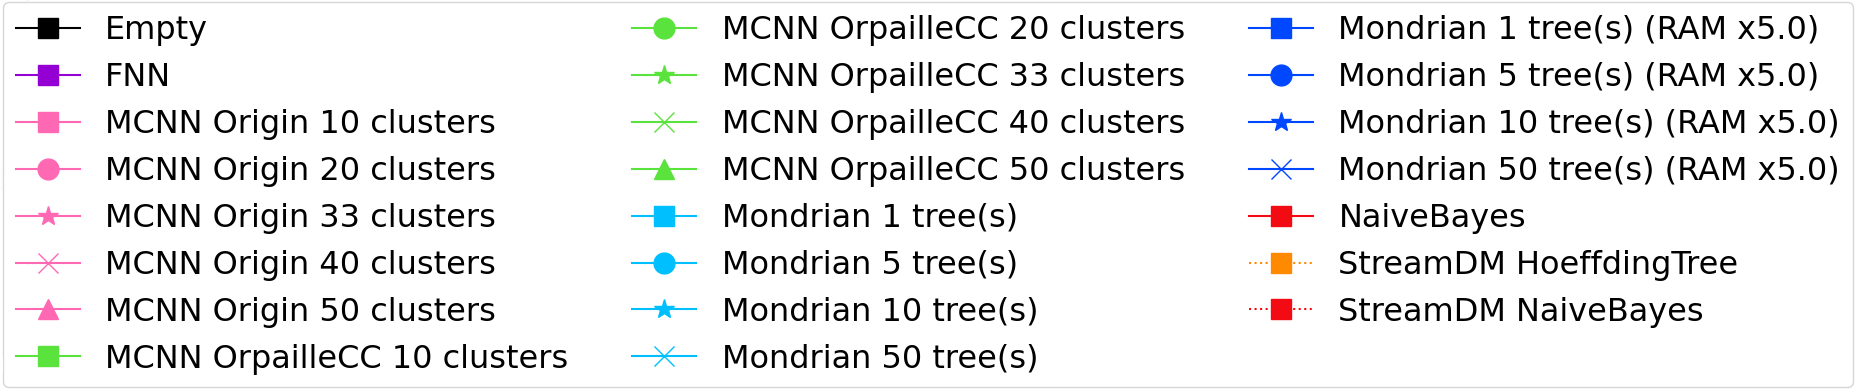
\includegraphics[width=0.8\linewidth]{figures/legend.png}
	\begin{subfigure}[t]{.49\linewidth}
		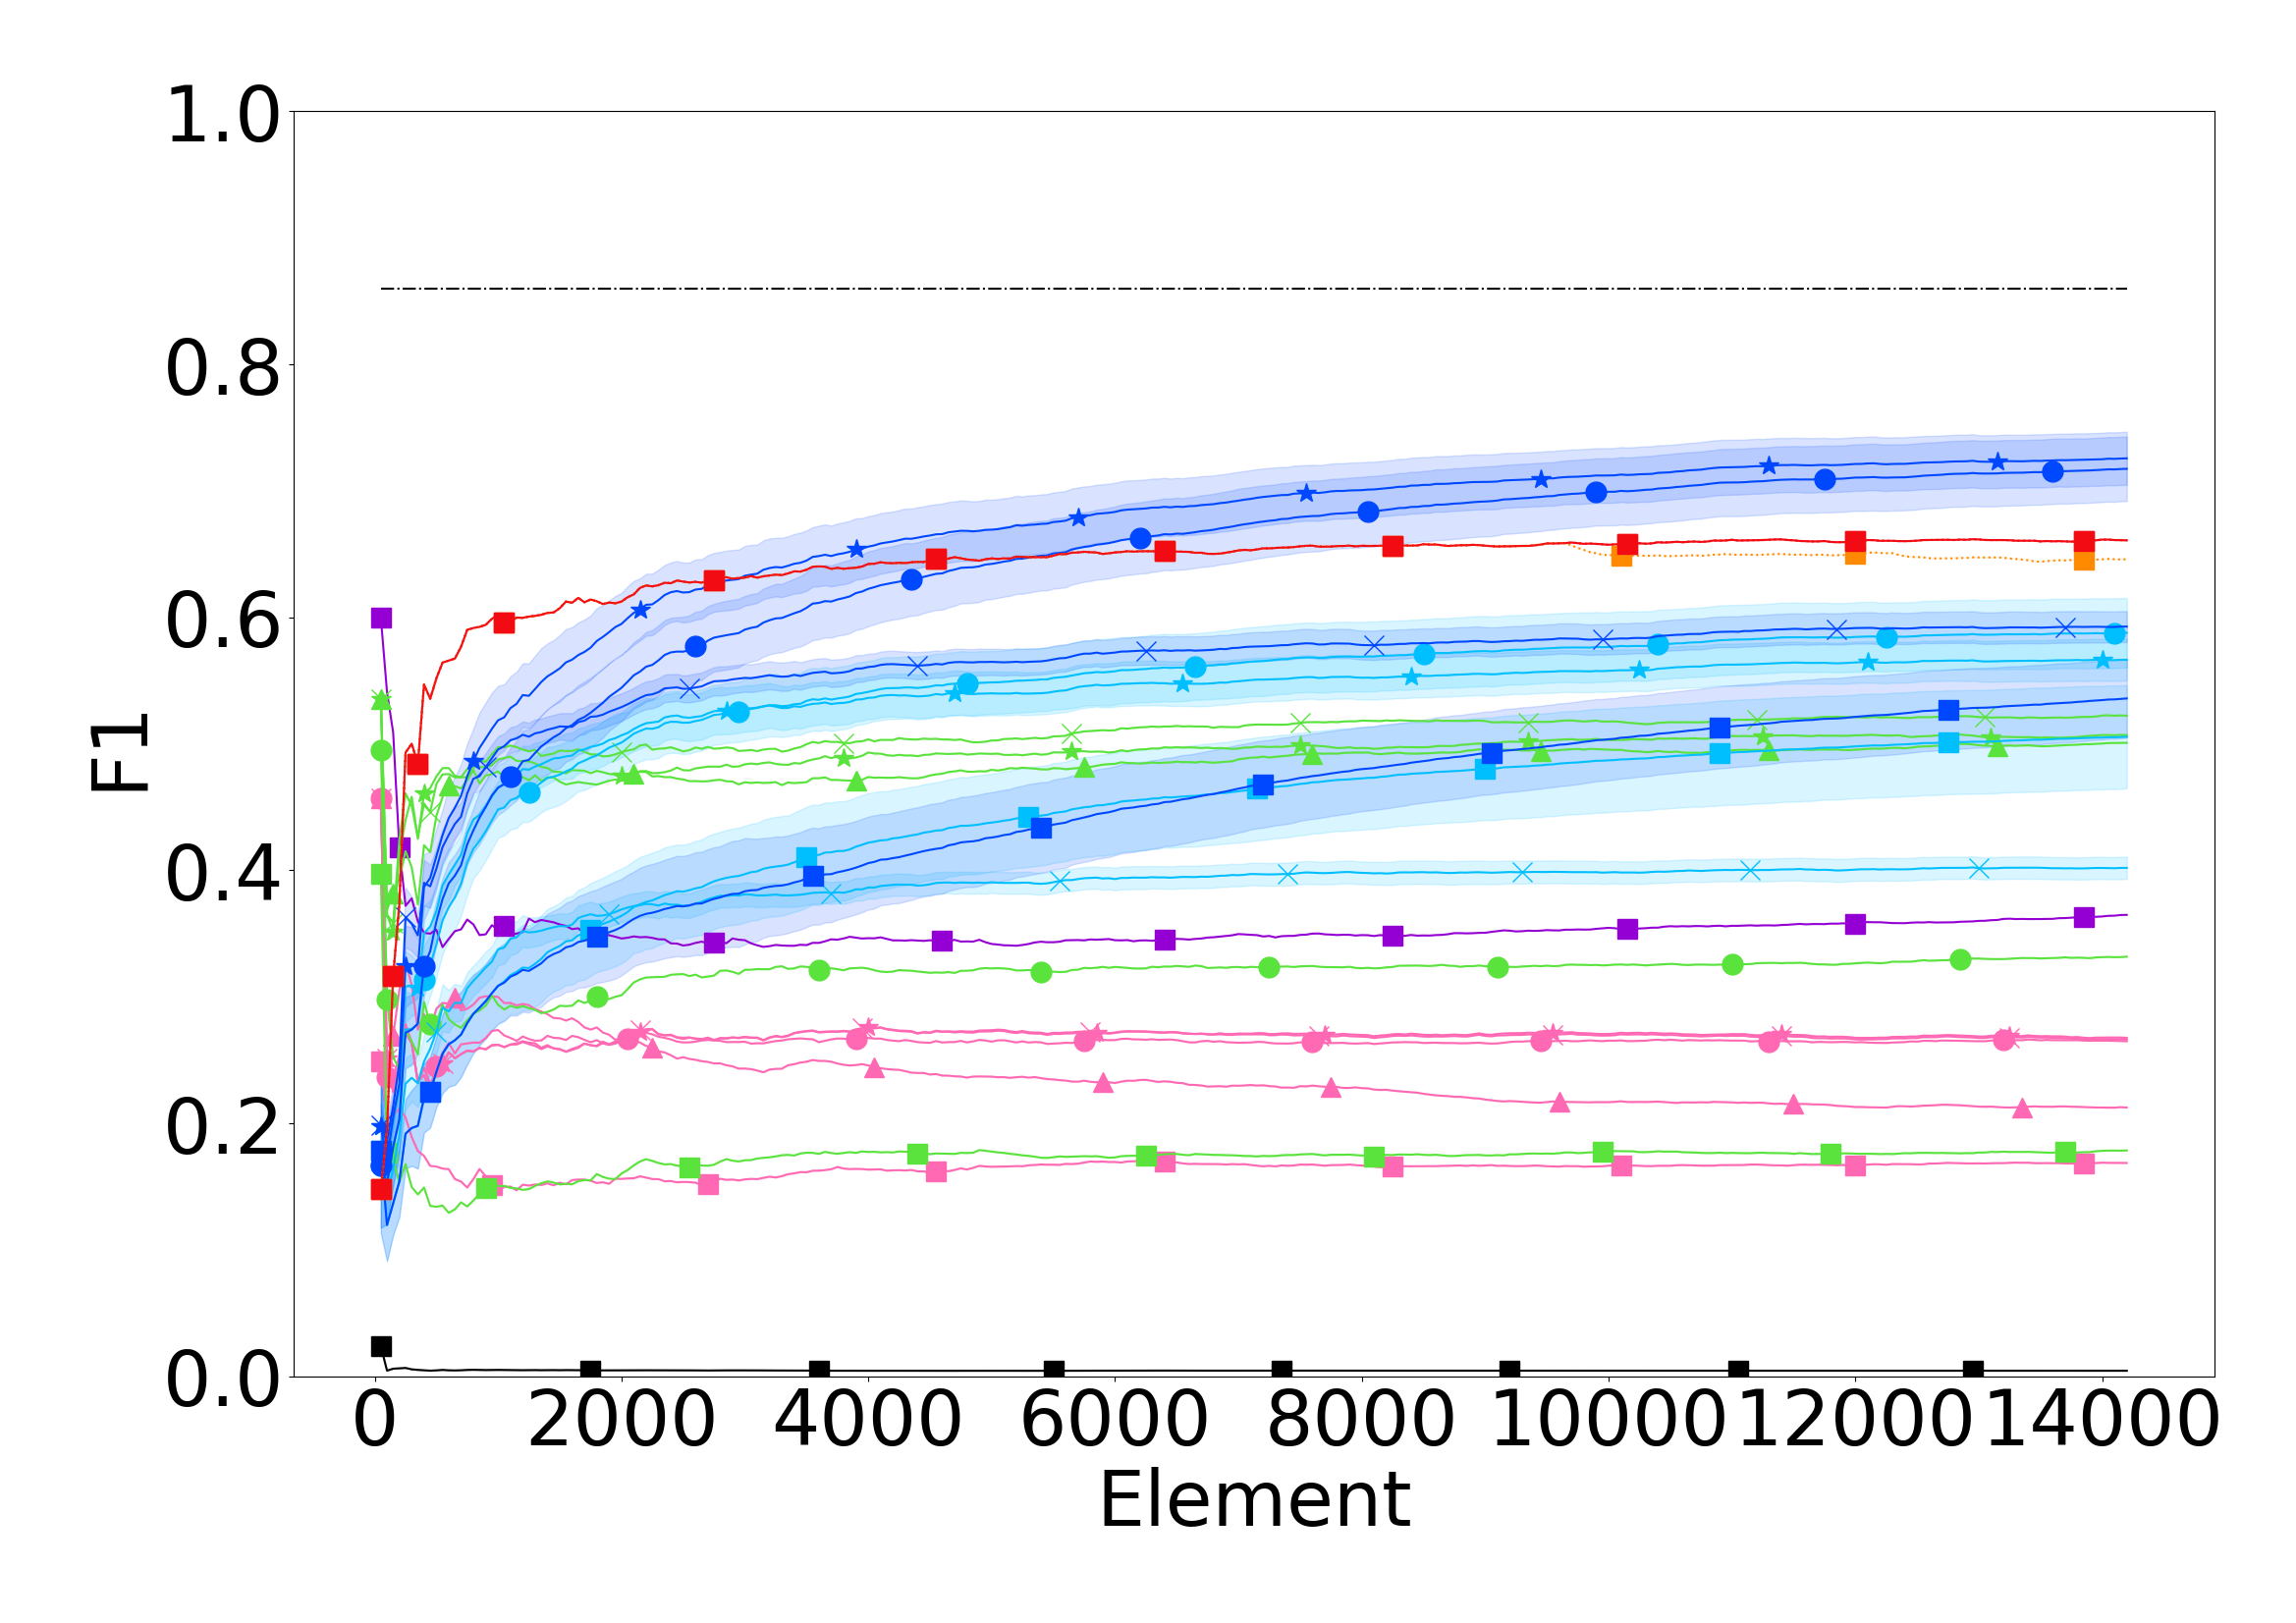
\includegraphics[width=\linewidth]{figures/results/banos_6_f1_std.png}
		\caption{\banosdataset}
		\label{fig:f1-banos}
	\end{subfigure}
	\begin{subfigure}[t]{.49\linewidth}
		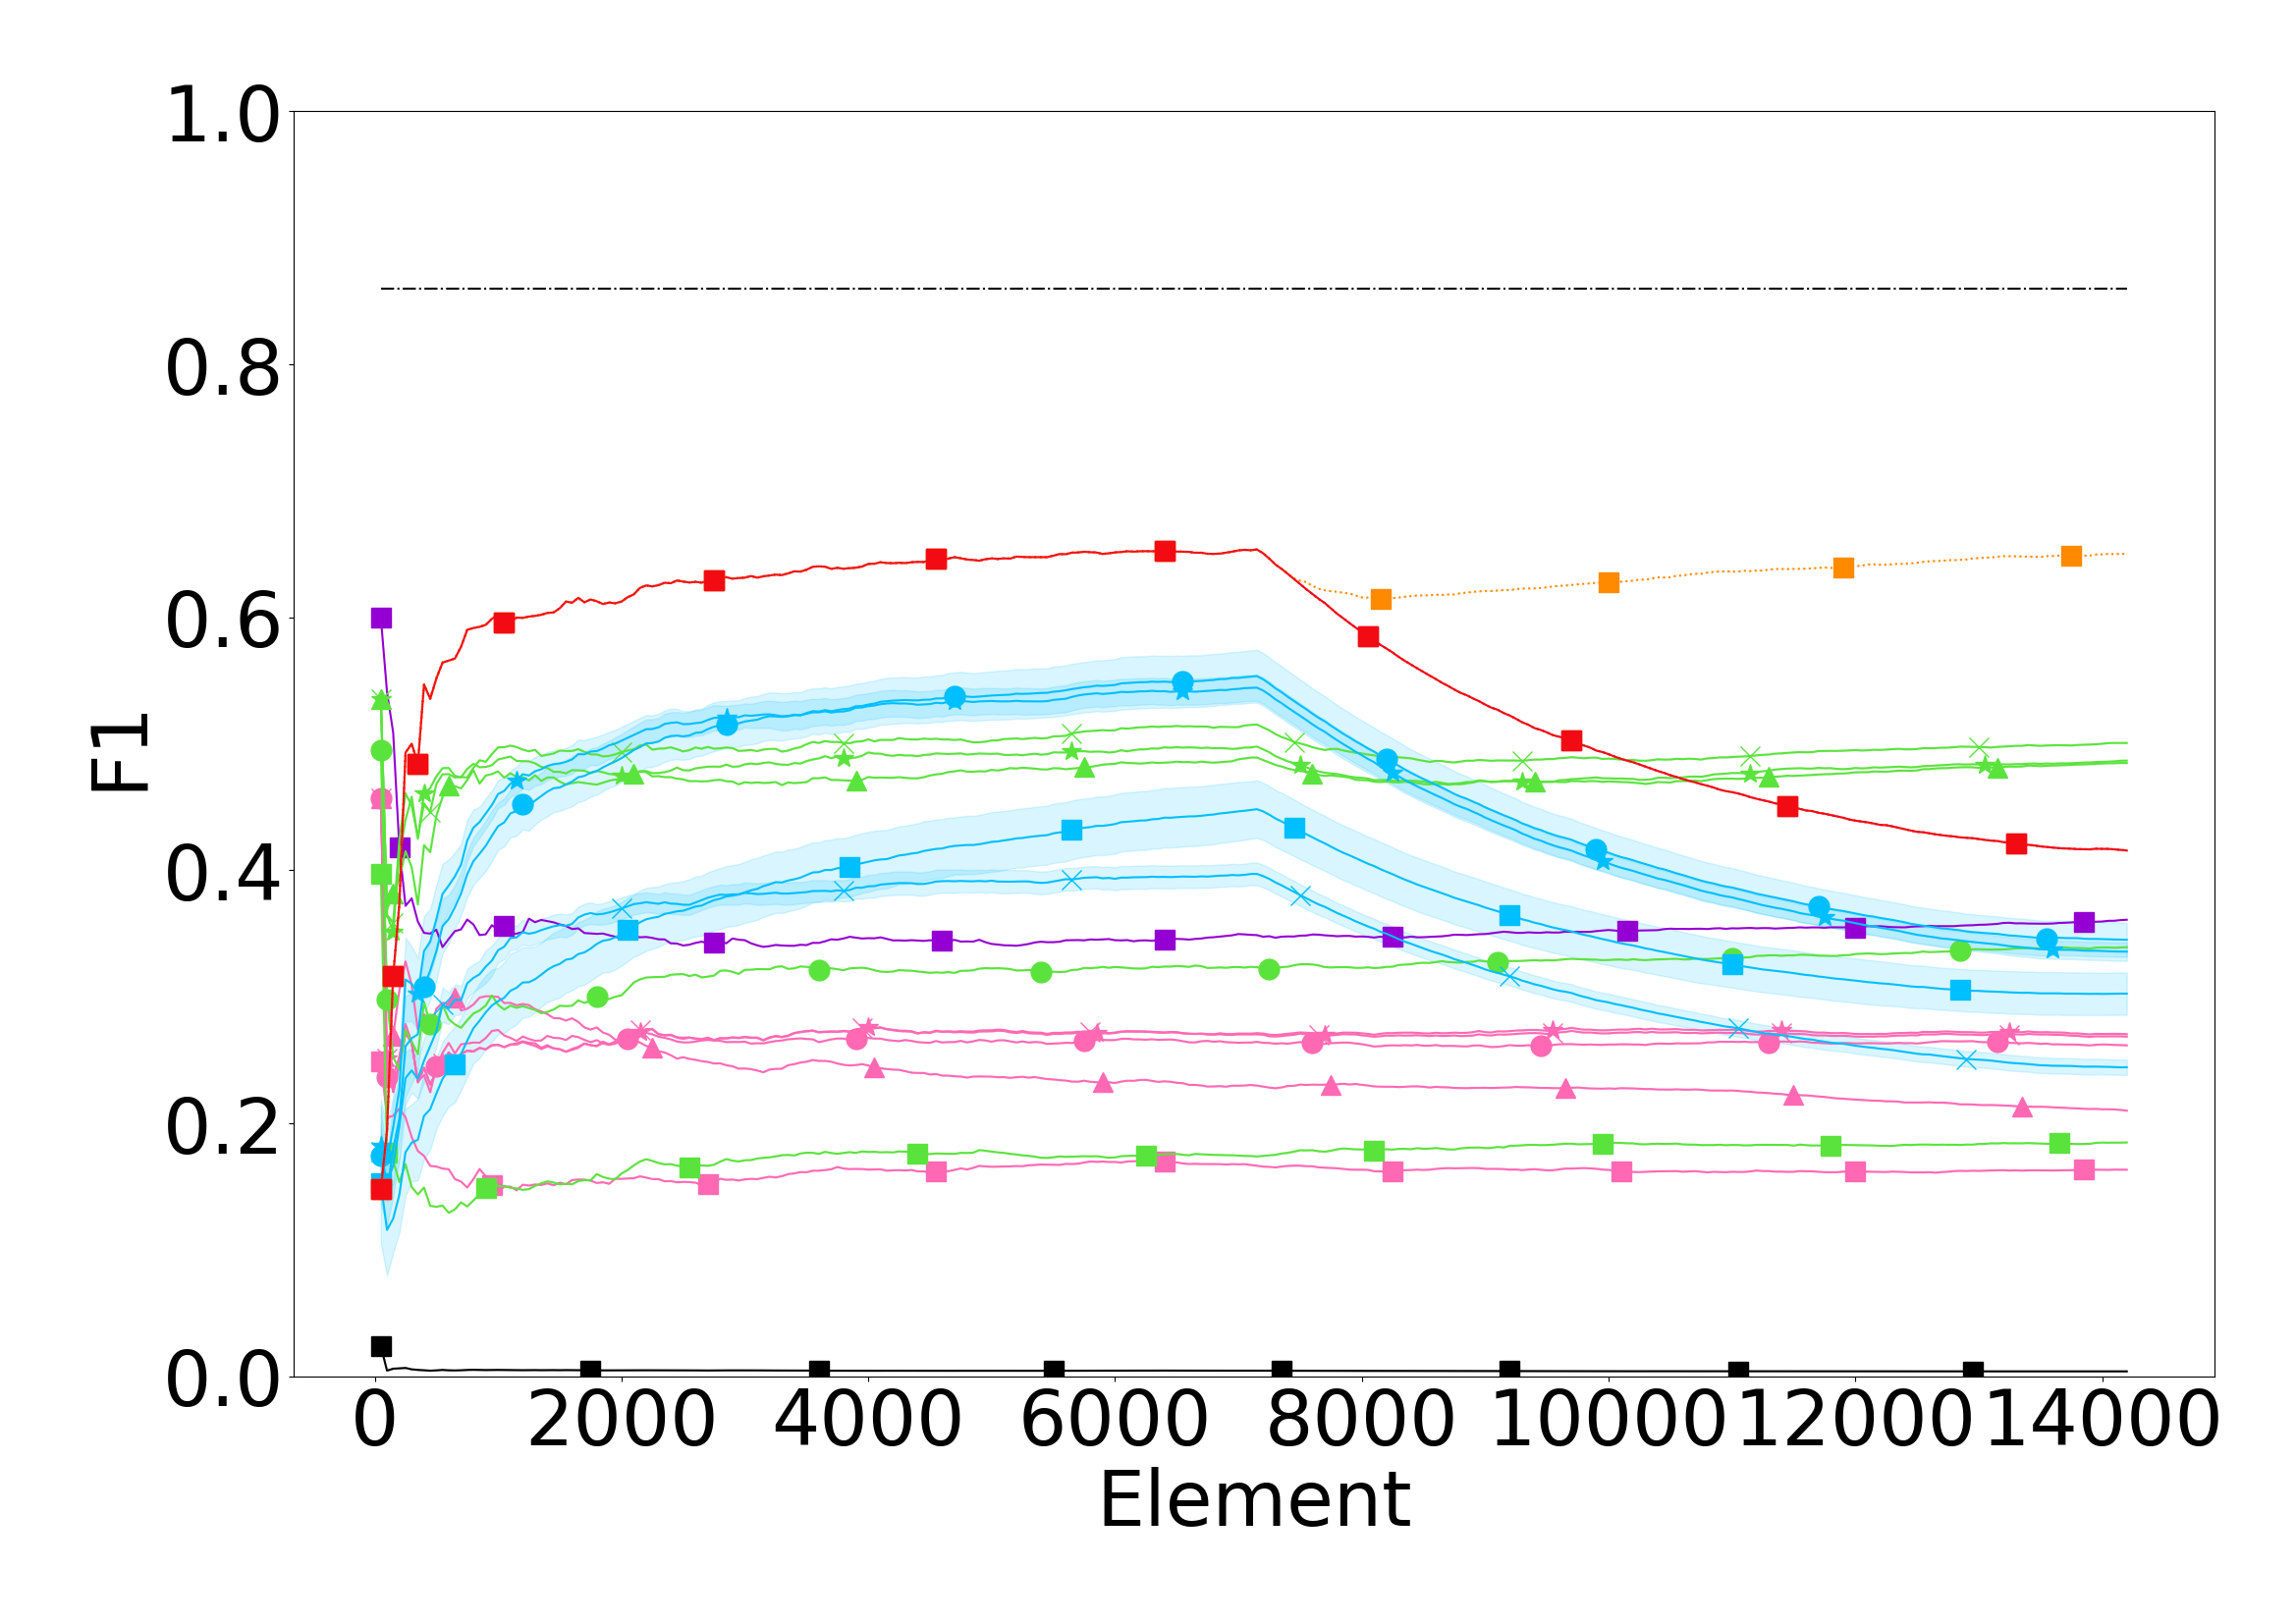
\includegraphics[width=\linewidth]{figures/results/drift_6_f1_std.png}
		\caption{\banosdataset (with Drift)}
		\label{fig:f1-drift}
	\end{subfigure}\\
	\begin{subfigure}[t]{.49\linewidth}
		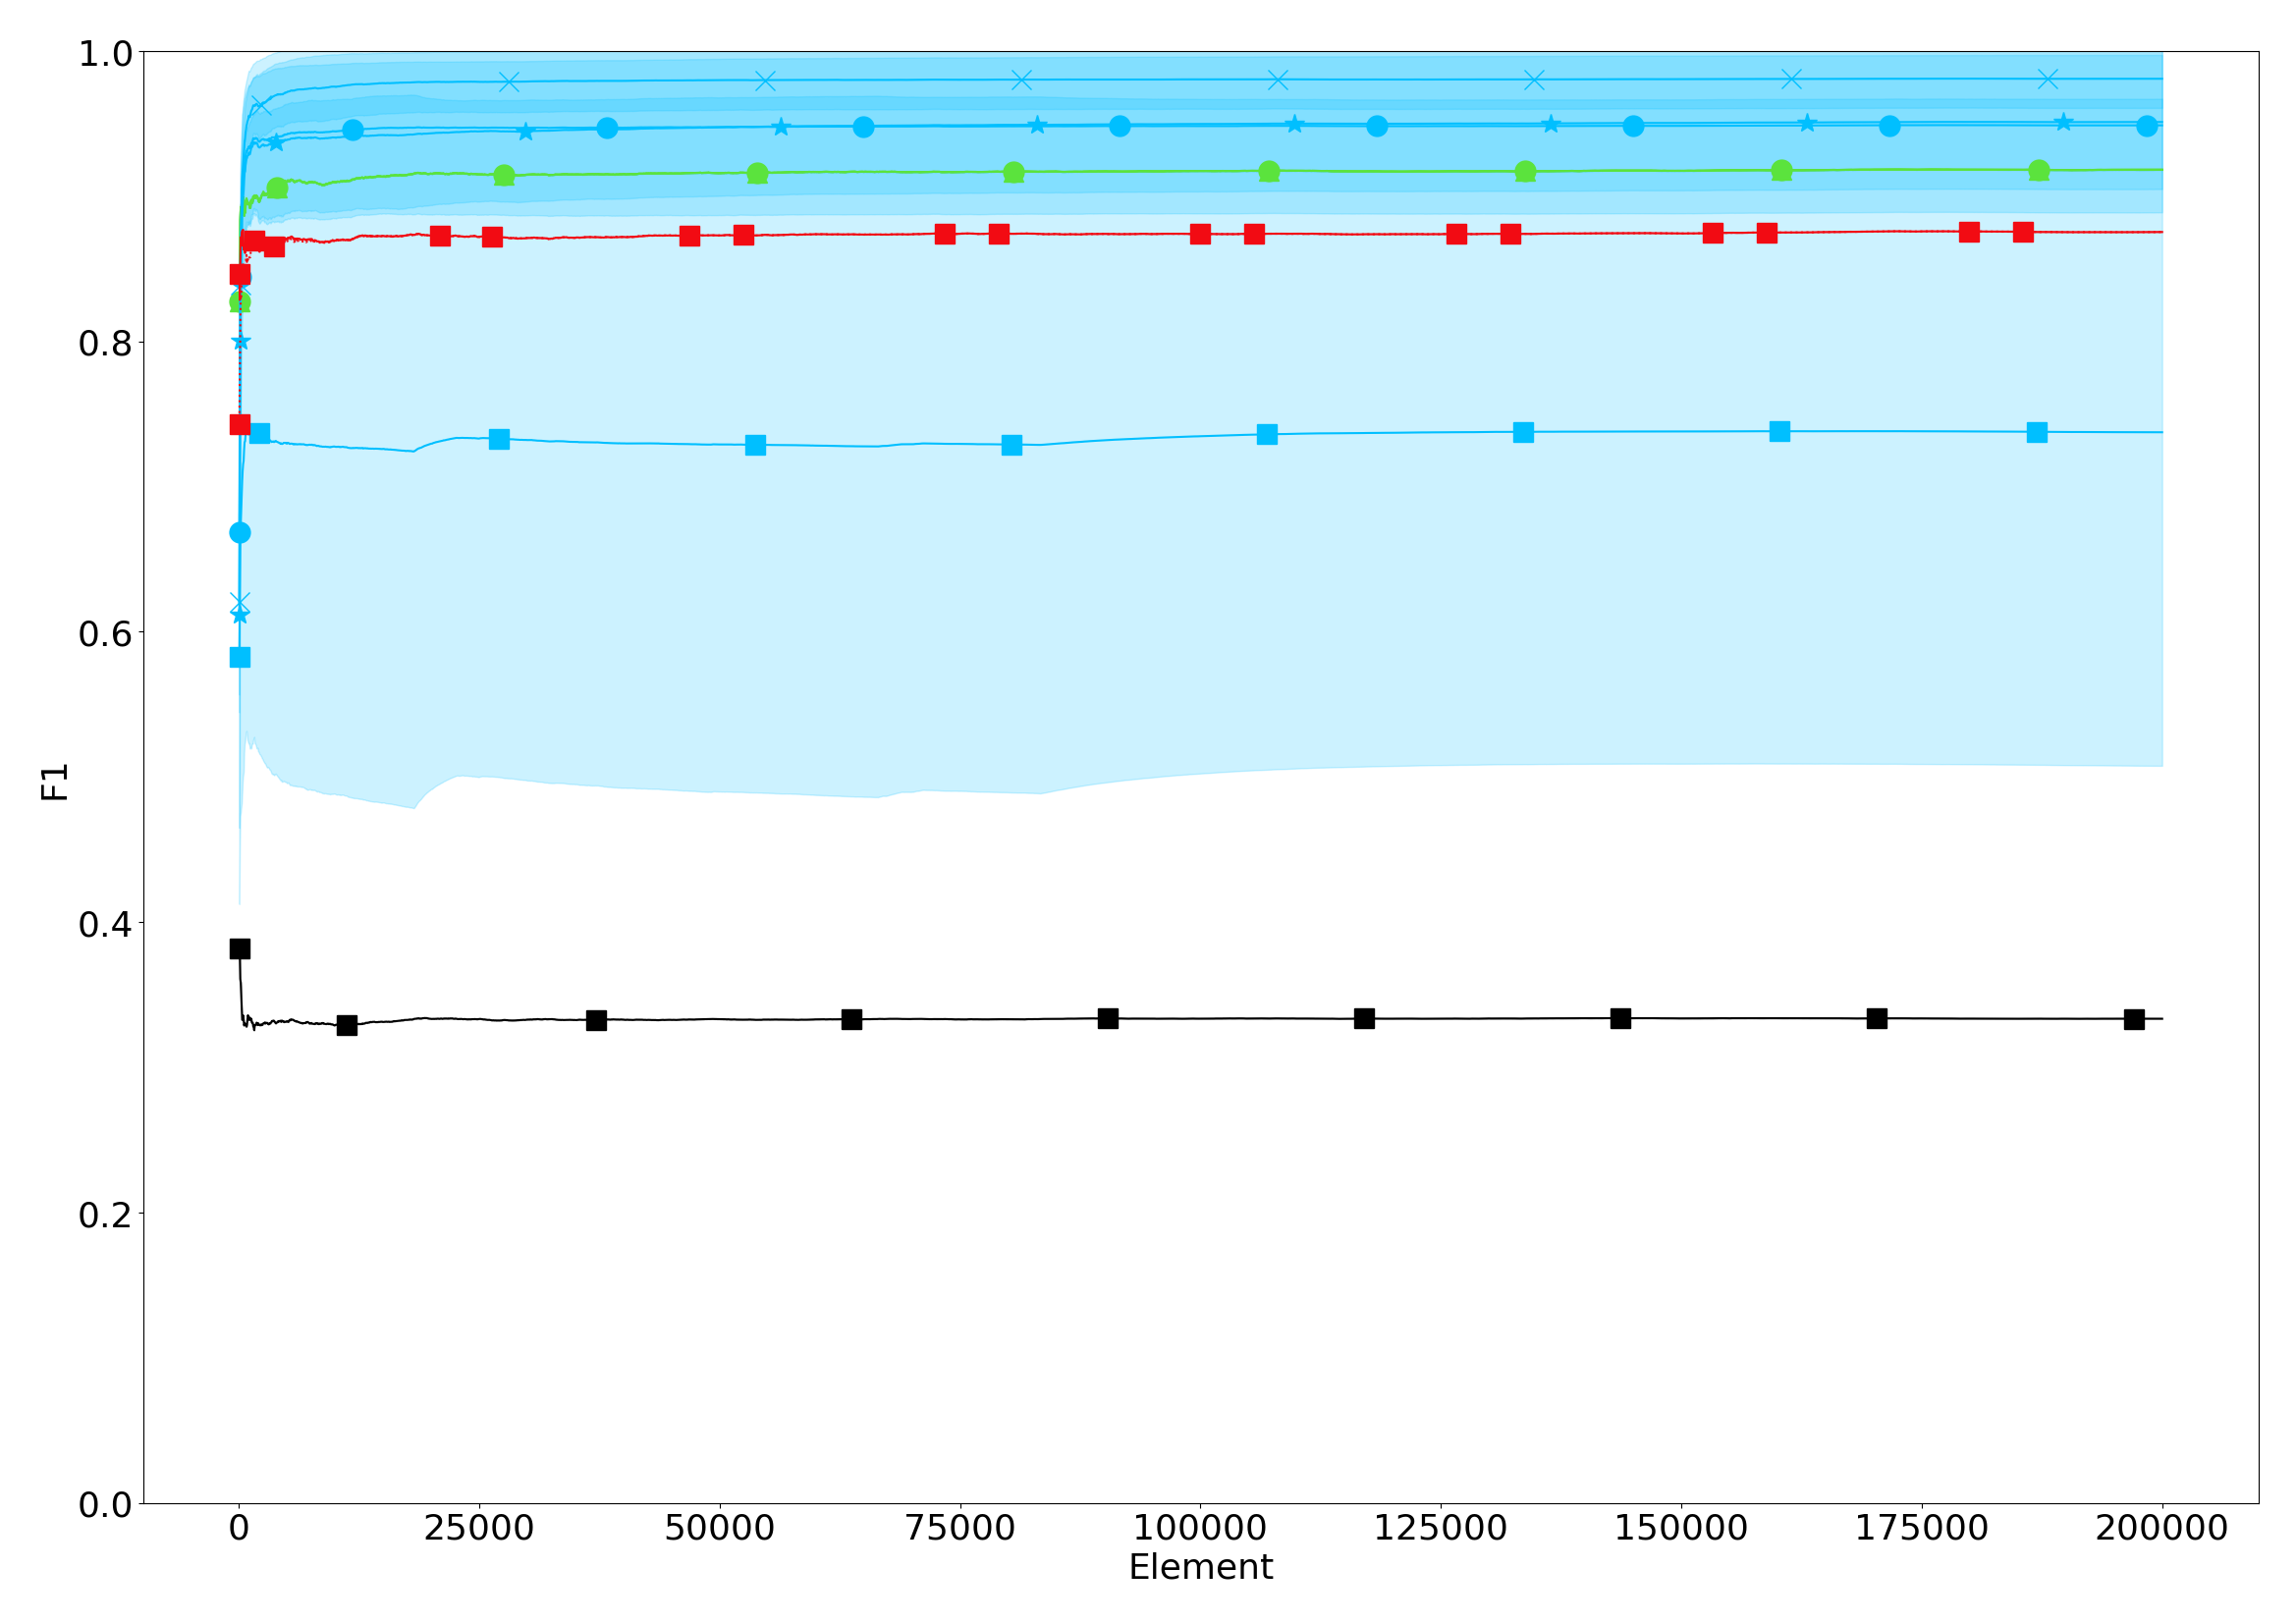
\includegraphics[width=\linewidth]{figures/results/dataset_1_f1_std.png}
		\caption{Hyperplane (MOA)}
		\label{fig:f1-dataset_1}
	\end{subfigure}
	\begin{subfigure}[t]{.49\linewidth}
		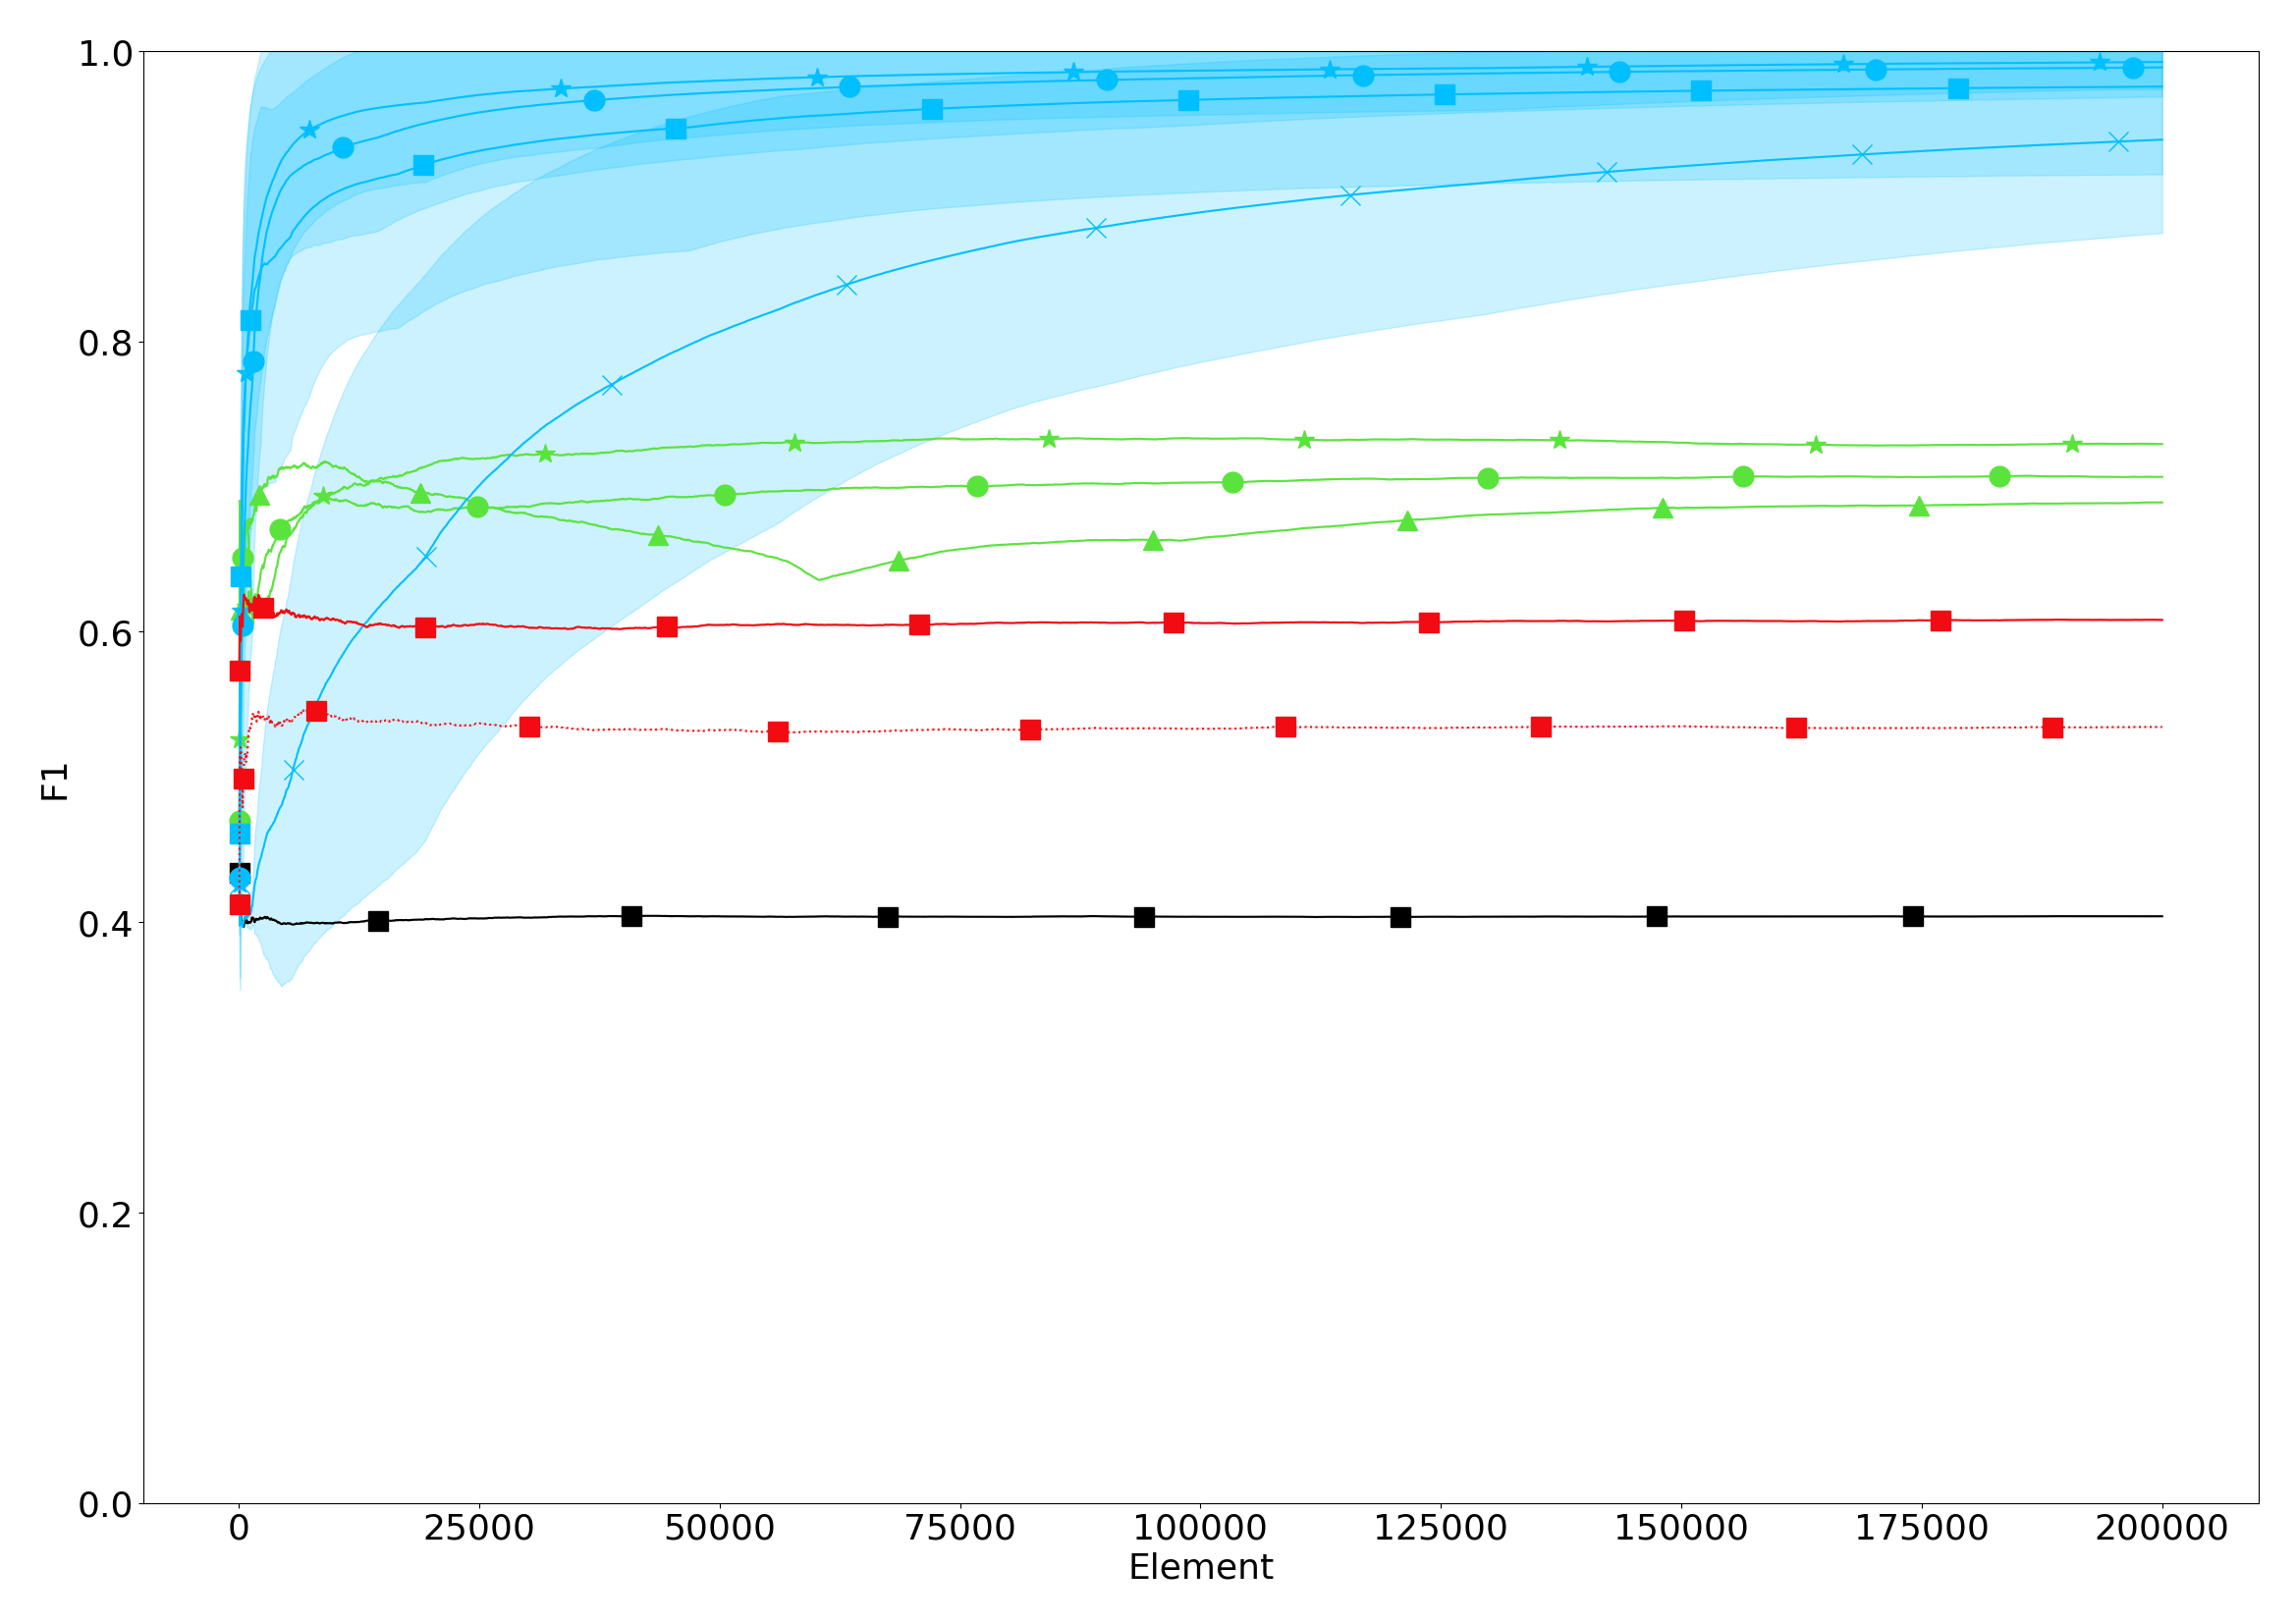
\includegraphics[width=\linewidth]{figures/results/dataset_2_f1_std.png}
		\caption{RandomRBF (MOA)}
		\label{fig:f1-dataset_2}
	\end{subfigure}\\
	\begin{subfigure}[t]{.49\linewidth}
		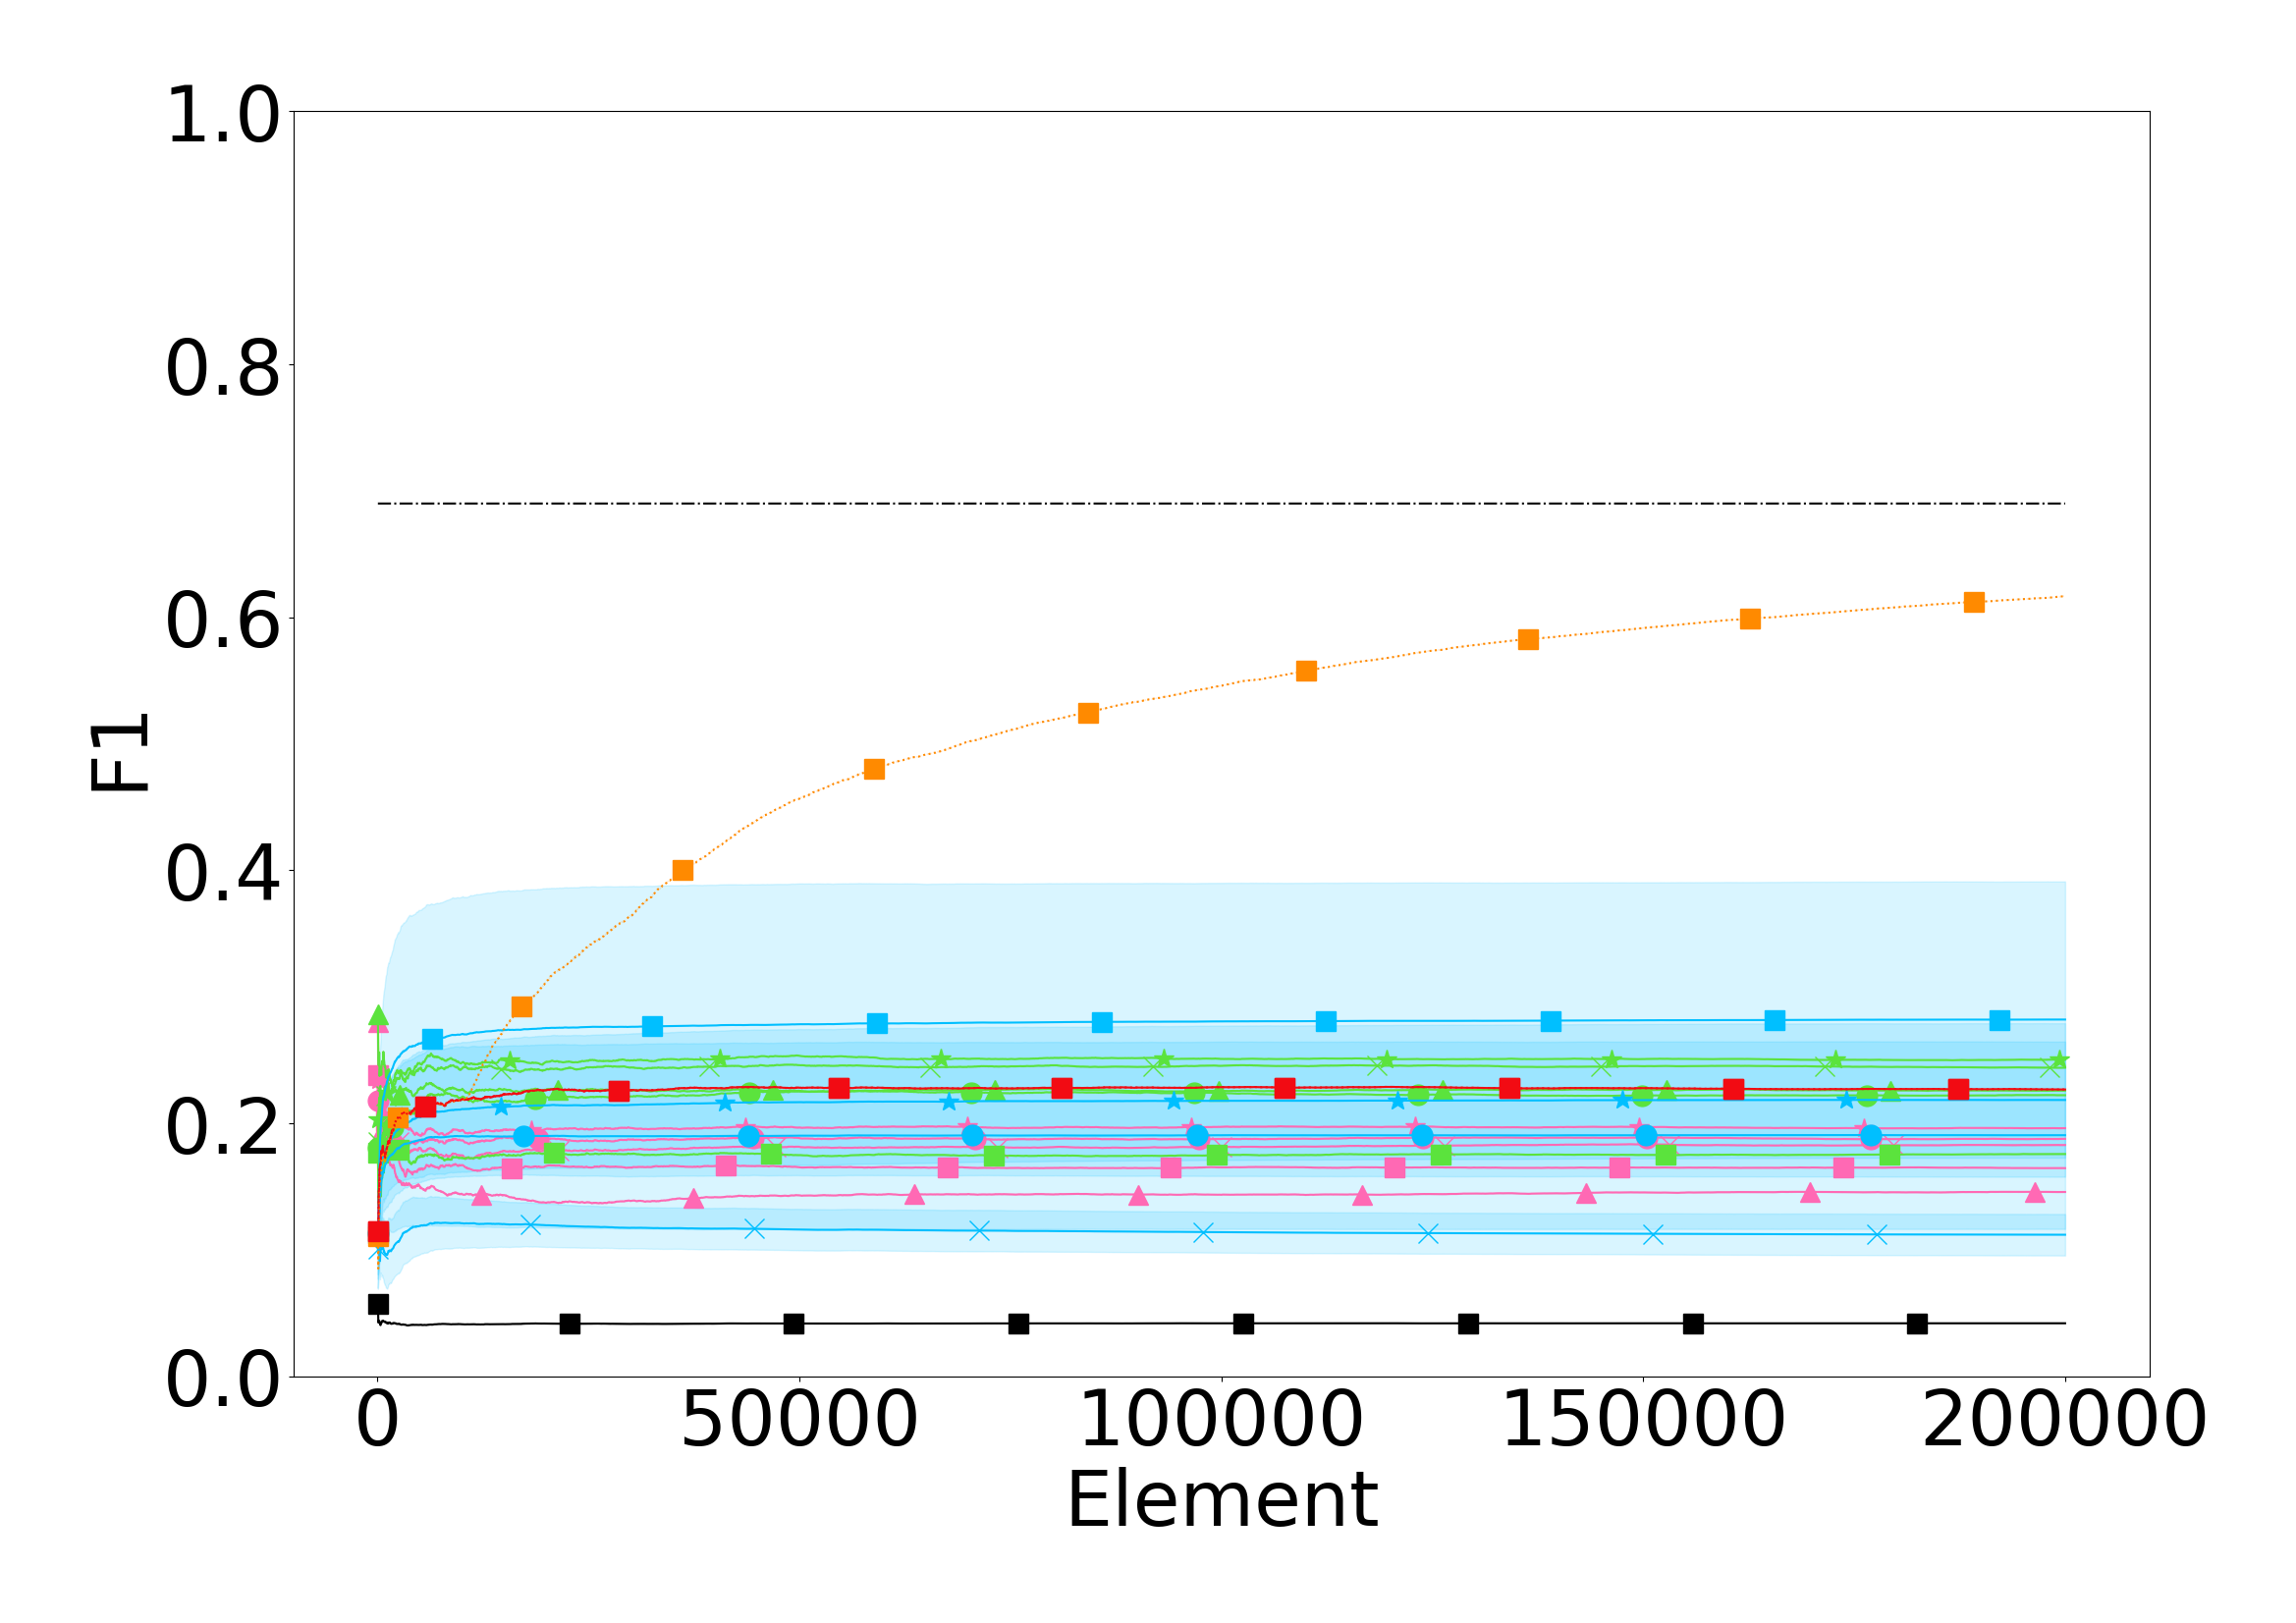
\includegraphics[width=\linewidth]{figures/results/dataset_3_f1_std.png}
		\caption{RandomTree (MOA)}
		\label{fig:f1-dataset_3}
	\end{subfigure}
	\begin{subfigure}[t]{.49\linewidth}
		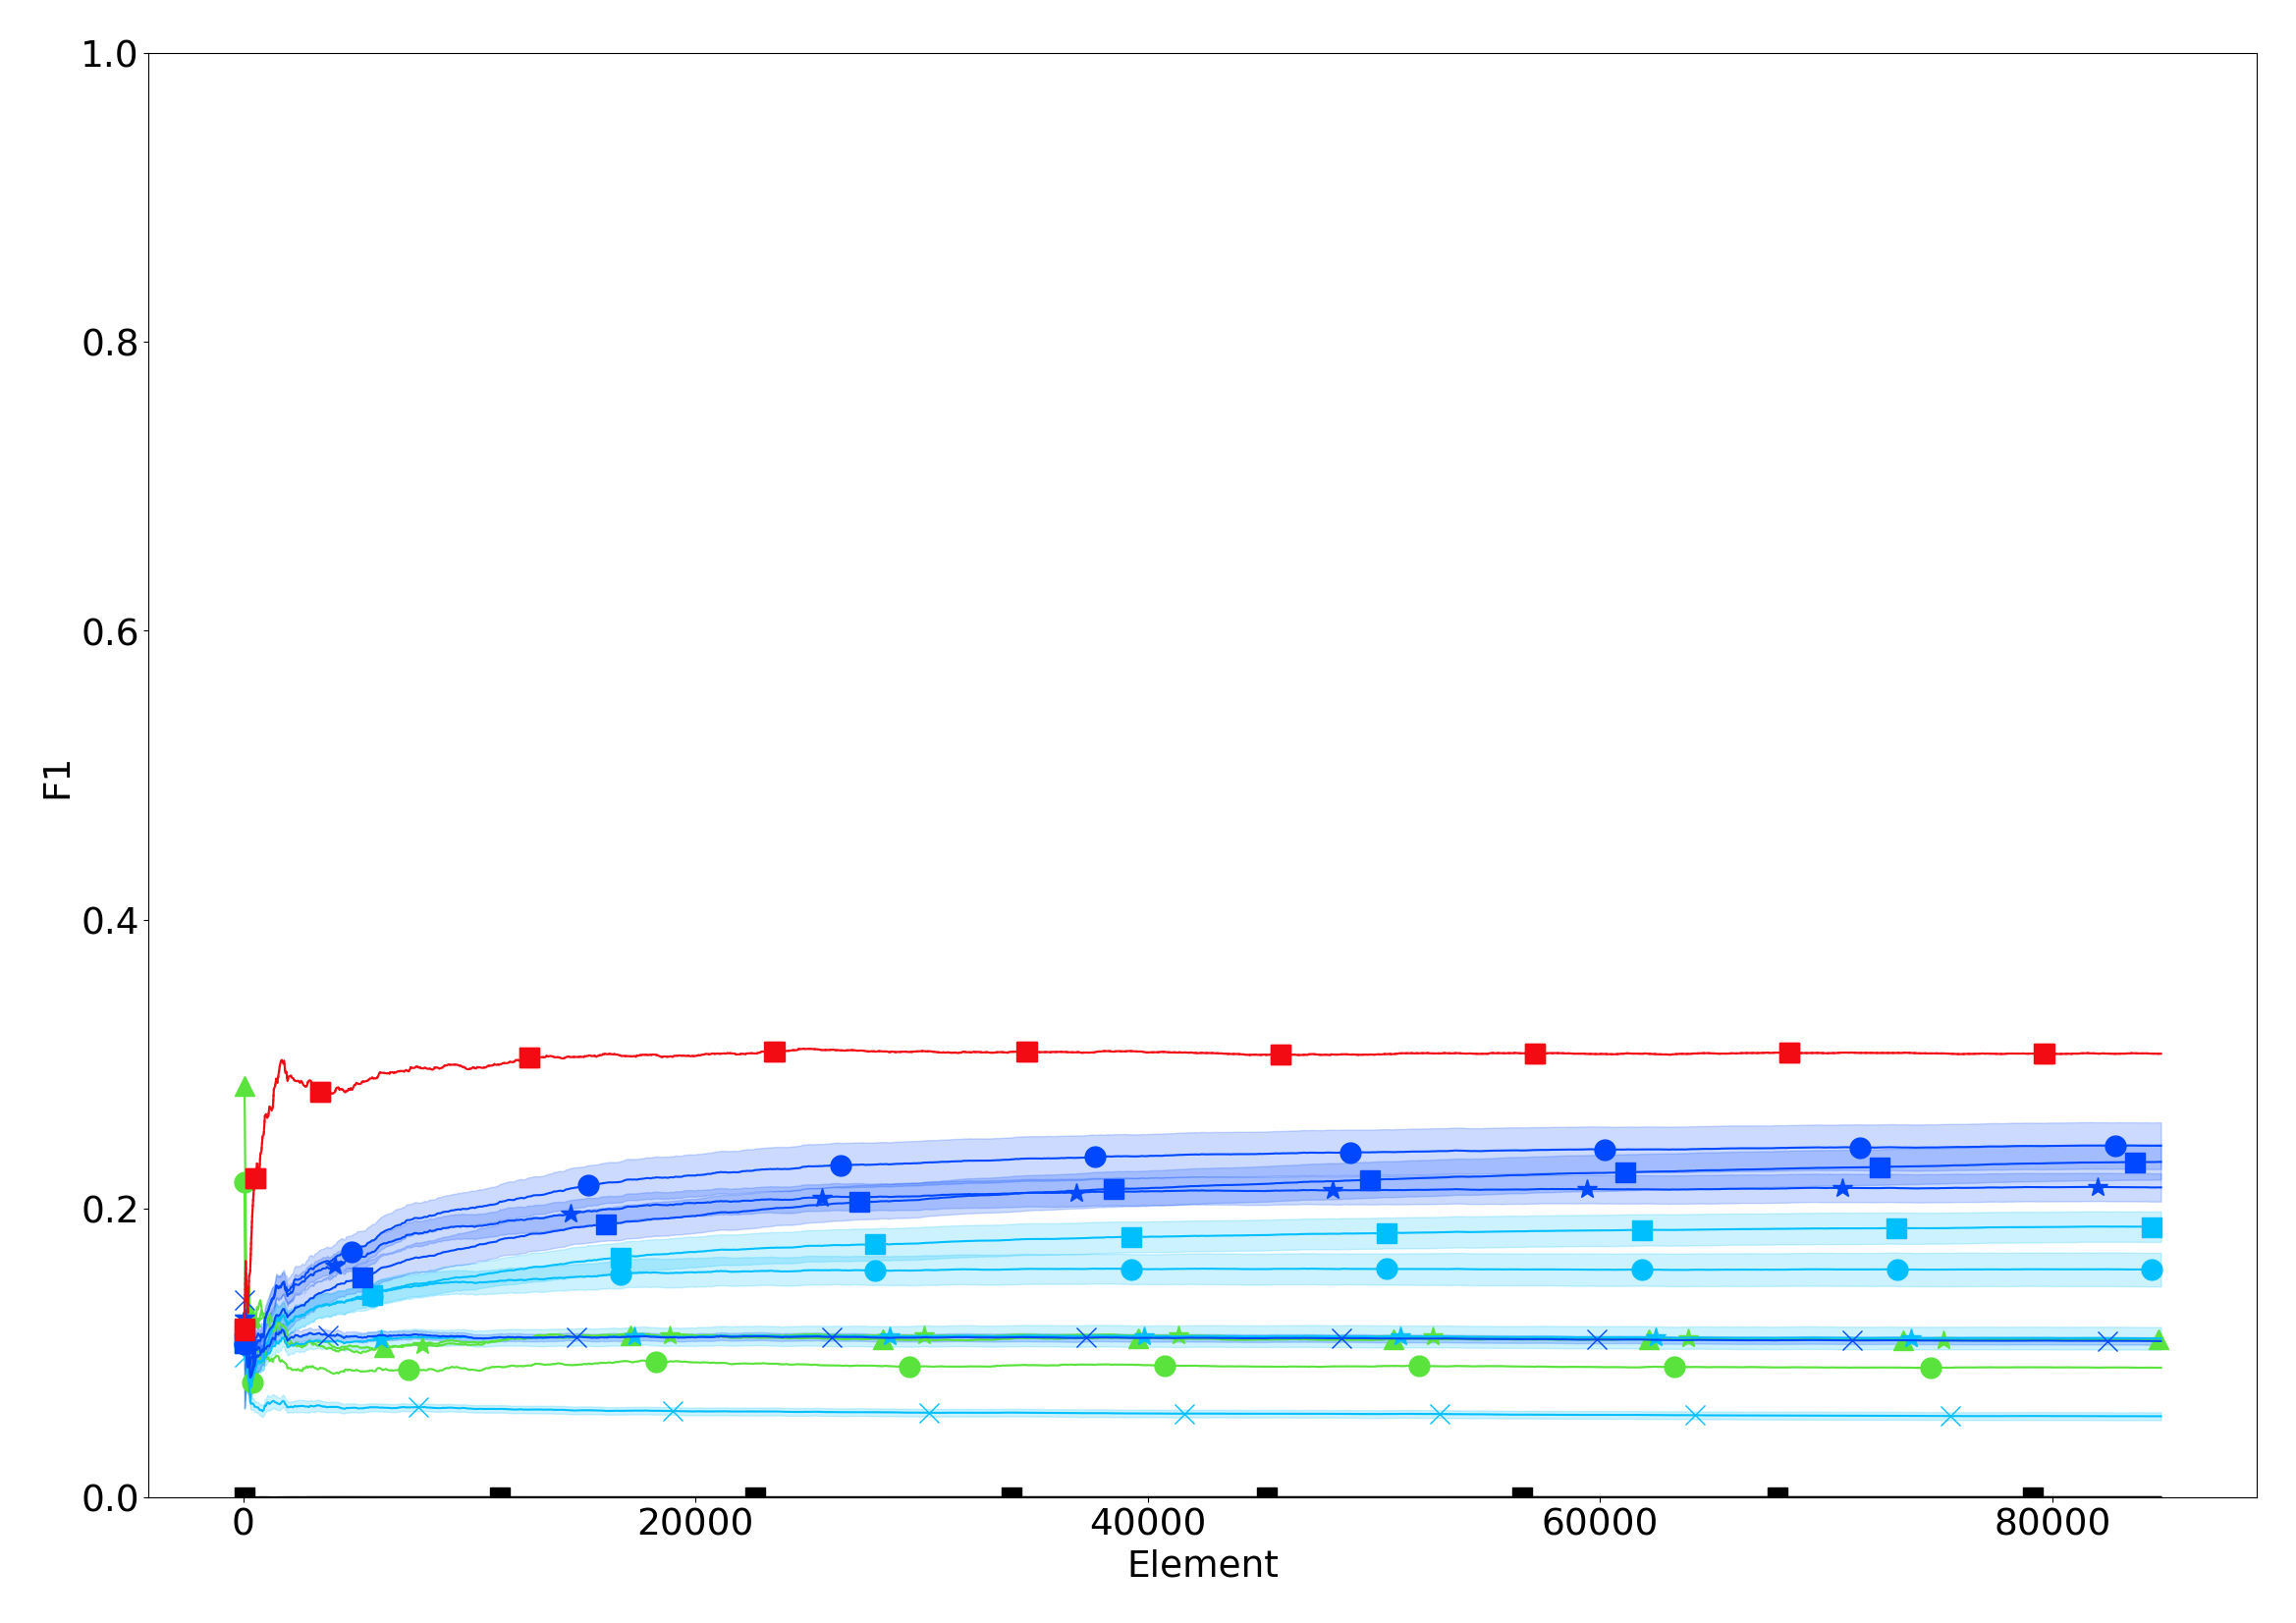
\includegraphics[width=\linewidth]{figures/results/recofit_6_f1_std.png}
		\caption{\recofitdataset}
		\label{fig:f1-recofit}
	\end{subfigure}
	\caption{F1 scores for the six datasets (average over 20 repetitions).
		The horizontal dashed black line indicates the offline \knn F1
		score (the value of k was obtained by grid search in [2, 20]). The
		blue shades represent a $\pm\sigma$ interval of the \mondrianforest
		classifier across repetitions.}
	\label{fig:f1}
\end{figure*}

\section{Results}
This section presents our benchmark results and the corresponding
hyperparameter tunning experiments.


\subsection{Overall classification performance}

%General description
Figure~\ref{fig:f1} compares the F1 scores obtained by all classifiers on
the six datasets. The graphs also show the standard deviation of the
\mondrianforest classifier observed across all repetitions (the other
classifiers do not involve any randomness). 

F1 scores vary greatly across the datasets. While the highest
observed F1 score is above 0.95 on the Hyperplane and RandomRBF datasets,
it barely reaches 0.65 for the \banosdataset dataset, and it remains under
0.40 on the \recofitdataset and RandomTree datasets. This trend is
consistent for all classifiers.

%Offline observations
The offline \knn classifier used as baseline achieves better F1 scores than
all other classifiers, except for the \mondrianforest on the Hyperplane and
the RandomRBF datasets. On the \banosdataset dataset, the difference of
\TG{x} with the best stream classifier remains very substantial, which
quantifies the remaining performance gap between data stream and offline
classifiers. On the \recofitdataset dataset, the difference between stream
and offline classifiers is lower, but the offline performance remains very
low.
%Recofit 9
%Banos 3
%Hyperplane 19
%RandomRBF 19
%RandomTree 15
%Drift 11

It should be noted that the F1 scores observed for the offline \knn
classifier on the real datasets are substantially lower than the values
reported in the literature. On the \banosdataset dataset, the original
study in~\cite{Banos_2014} reports an F1 score of 0.96, the work
in~\cite{behzad2019} achieves 0.92, but our benchmark only achieves 0.86.
Similarly, on the \recofitdataset dataset, \TG{check original study} the
work in~\cite{behzad2019} reaches 0.65 while our benchmark only achieves
0.40. This is most likely due to our use of data coming from a single
sensor, consistently with our motivating use case, while the other works used mutiple ones (\TG{x} in the case of
\banosdataset, \TG{y} in the case of \recofitdataset).

% %One sensor
% In this study, we focused on using one sensor rather than all the sensors
% available in the real datasets. In the case of more sensor used, we would expect
% an F1 score improvement for all classifiers because they would have access to
% more data in order to discriminate the classes. 
% On the other hand, we would
% expect an increase in the memory footprint because more sensors mean more
% attribute extracted. 
% This should have minimal impact on classifiers such as
% \naivebayes because their footprint is already low. However, the
% \mondrianforest, the \hoeffdingtree, and \mcnn memory footprints are expected to
% grow significatively because more sensors means more attributes for each leaf or
% cluster. In particular, we expect the \mondrianforest F1 score to be mitigated
% by the decrease of memory induced by the increased leave size \TG{Merge in second paragraph of sub-section A.}.

%Concept drift
The \hoeffdingtree appears to be the most robust to concept drifts
(\banosdataset (with drift)), while the \mondrianforest and \naivebayes
classifiers are the most impacted. \mcnn classifiers are marginally impacted.
The low resilience of \mondrianforest to concept drifts can be attributed to
two factors. First, existing nodes in trees of a \mondrianforest cannot be updated.
Second, when the memory limit is reached, \mondriantrees cannot grow
or reshape their structure anymore.


\subsection{\hoeffdingtree and \naivebayes}

%Hoeffding and Naïve Bayes description when they are the best
The \naivebayes and the \hoeffdingtree classifiers stand out on the two real datasets
(\banosdataset and \recofitdataset) even though the F1 scores observed remain
low (0.6 and 0.35) compared to offline \knn (0.86 and 0.40). Additionally, the
\hoeffdingtree performs outstandingly on the RandomTree dataset and
\banosdataset dataset with a drift. Such good performances where expected on the
RandomTree dataset because it was generated based on a tree structure, however

%Explanation of their F1 score similarity
Except for the \banosdataset dataset, the \hoeffdingtree performs better
than \naivebayes. For all datasets, the performance of both classifiers is
comparable at the beginning of the stream, because the \hoeffdingtree uses
a \naivebayes in its leaves.  However, F1 scores diverge throughout the
stream, most likely because of the \hoeffdingtree's ability to reshape its
tree structure.  This occurs after a sufficient amount of elements, and the
difference is more noticeable after a concept drift.

%Naive Bayes and Naive Bayes
Finally, we note that the StreamDM and OrpailleCC implementations of
\naivebayes are indistinguishable from each other, which confirms our
implementation in OrpailleCC.

\subsection{\mondrianforest}

%Mondrian when at best
On two synthetic datasets, Hyperplane and RandomRBF, the \mondrianforest (RAM x
1.0) with 10 trees achieves the best performance (F1$>$0.95), above the offline
\knn.  Additionally, the \mondrianforest with 5 or 10 trees ranks third on the
two real datasets. 

%Mondrian discussion
Surprisingly, a \mondrianforest with 50 trees performs worse than 5 or 10
trees on most datasets. The only exception is the Hyperplane dataset where
50 trees perform between 5 and 10 trees. This is due to the fact that
our \mondrianforest implementation is memory bounded, which is
useful on connected objects but limits tree growth when the allocated memory is
full. Because 50 trees fill the memory faster than 10 or 5 trees, the
learning stops earlier, before the trees can learn learned enough from the
data. It can also be noted that the variance of the F1 score decreases with
the number of trees, as expected.

%Mondrian RAMx5
This dependency of the \mondrianforest to memory allocation is shown in
\banosdataset and \recofitdataset datasets, where an additional
configuration with five times more memory than the initial configuration is
shown (total of 3~MB).  The memory increase induces an F1 score difference
greater than 0.1, except when only one tree is used, in
which case the improvement caused by the memory is less than 0.05. Note that the
selected memory bound may not be achievable on a connected object. Overall,
\mondrianforest seems to be a viable alternative to \naivebayes or the
\hoeffdingtree for \har.


\subsection{\mcnn}

%MCNN observations
The \mcnn OrpailleCC stands out on \banosdataset (with drift) dataset where it
ranks second thanks to its adaptation to the concept drift.  On other datasets,
\mcnn OrpailleCC ranks below the \mondrianforest and the \hoeffdingtree, but
above \mcnn Original. This difference between the two \mcnns is presumably due
to the fact that \mcnn Origin removes clusters with low participation too early.
On the real datasets (\banosdataset and \recofitdataset), we notice that the
\mcnn OrpailleCC appears to be learning faster than the \mondrianforest,
although the \mondrianforest catches up after a few thousand elements. Finally,
we note that \mcnn remains quite lower than the offline \knn.

\subsection{\FNN}

%FNN observation
Figure~\ref{fig:f1-banos} shows that the \FNN has a low F1 score (0.36)
compared to other classifiers (above 0.5), which contradicts the results
reported in~\cite{omid_2019} where the \FNN achieves more than 95\%
accuracy in a context of offline training. The main difference
between~\cite{omid_2019} and our study lies in the definition of the
training set. In~\cite{omid_2019}, the training set includes examples from
every subject, while we only use a single one, to ensure an objective
comparison with the other stream classifiers that do not require offline
training (except for hyperparameter tuning, done on the first subject of
the \banosdataset dataset). When we use a random sample of 10\% of the
datapoints across all subjects for offline training, we reach an F1 score
of 0.62 \TG{check value}, which is closer to the performance of the
\naivebayes classifier.

%FNN discussion
%As explained in Section~\ref{sec:method-fnn}, the pre-training of the \FNN is
%slightly different other classifiers. Indeed, the hyperparameters tuning of the
%other classifiers implies that they start the testing phase with no prior
%knowledge of the dataset, even about the element seen in the tuning phase. On
%the other hand, the \FNN starts with its weights already set from the training
%phase, therefore it has already seen datapoints from the first subject. This
%procedure genuinely helps the \FNN, otherwise the random weights would force the
%F1 score down, closer to the empty classifier.  Additionally to the
%pre-training, we used feature extraction from~\cite{omid_2019} which exhibits
%high classification performance.  Since we only trained the \FNN on the first
%subject of \banosdataset dataset, we could not apply the same neural network
%structure on other datasets.

\begin{figure*}
	\begin{subfigure}[t]{.49\linewidth}
		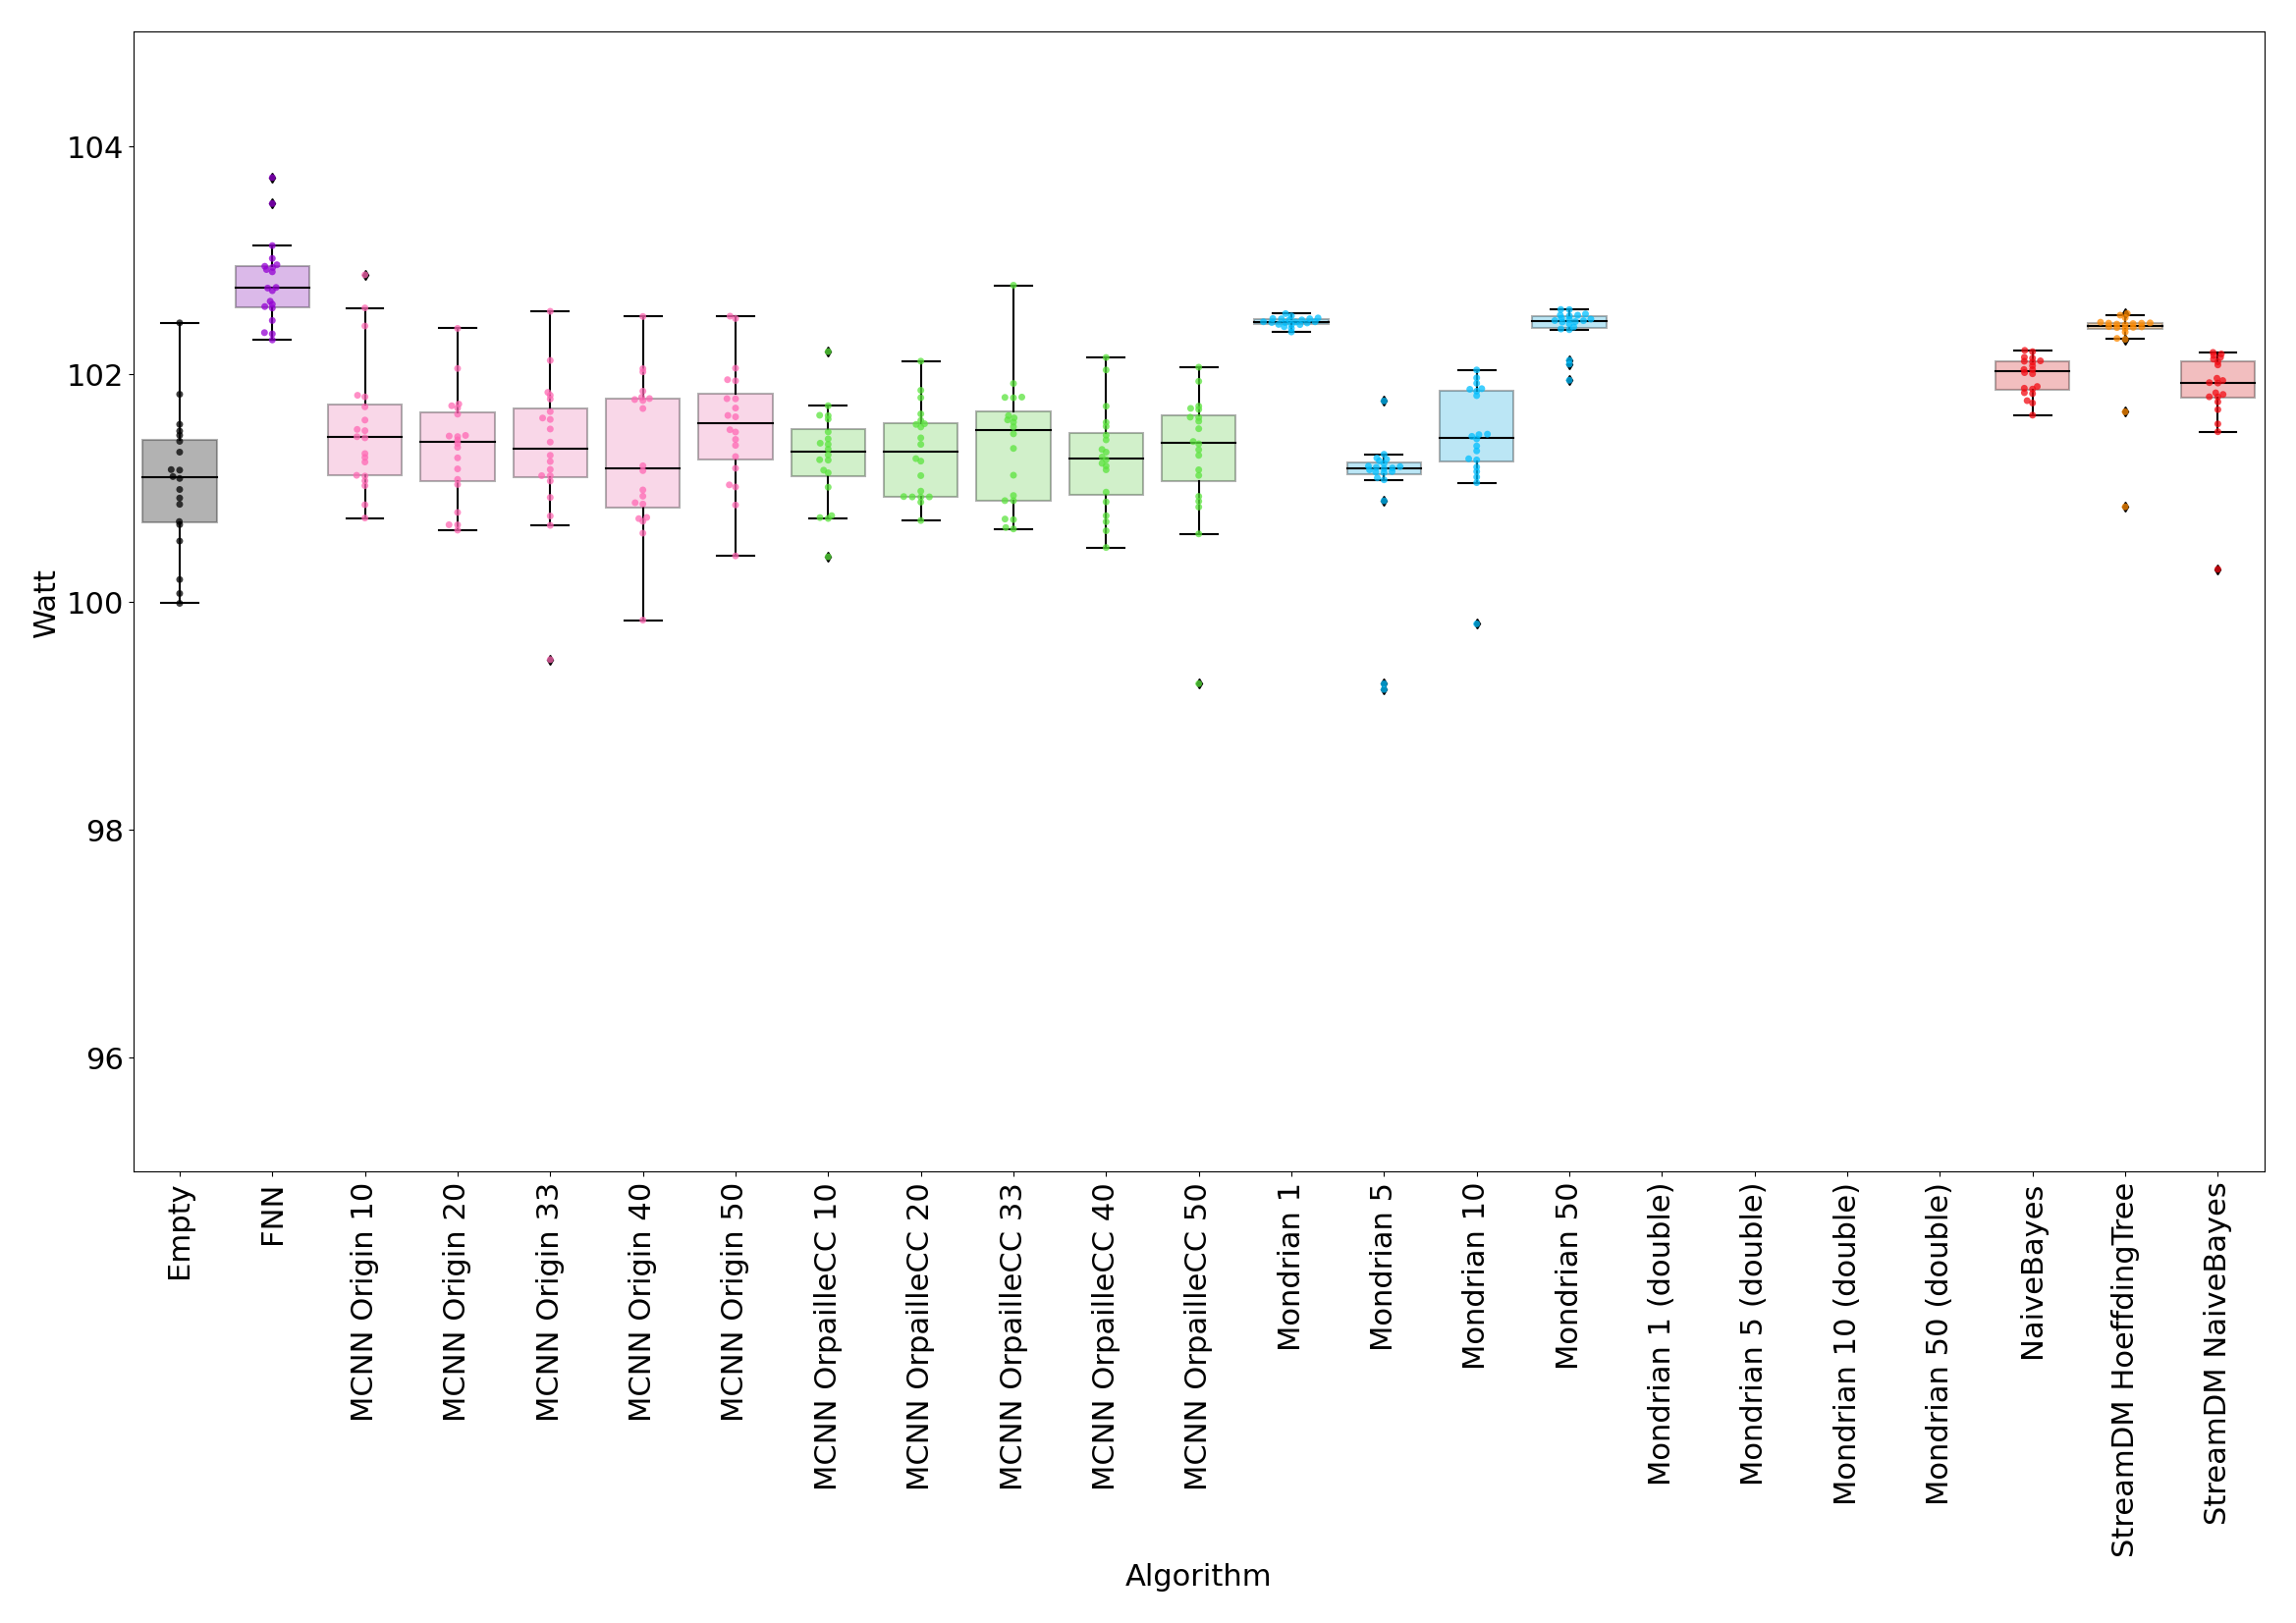
\includegraphics[width=\linewidth]{figures/results/banos_3_watt.png}
		\caption{\banosdataset}
		\label{fig:power-banos}
	\end{subfigure}
	\hfill
	\begin{subfigure}[t]{.49\linewidth}
		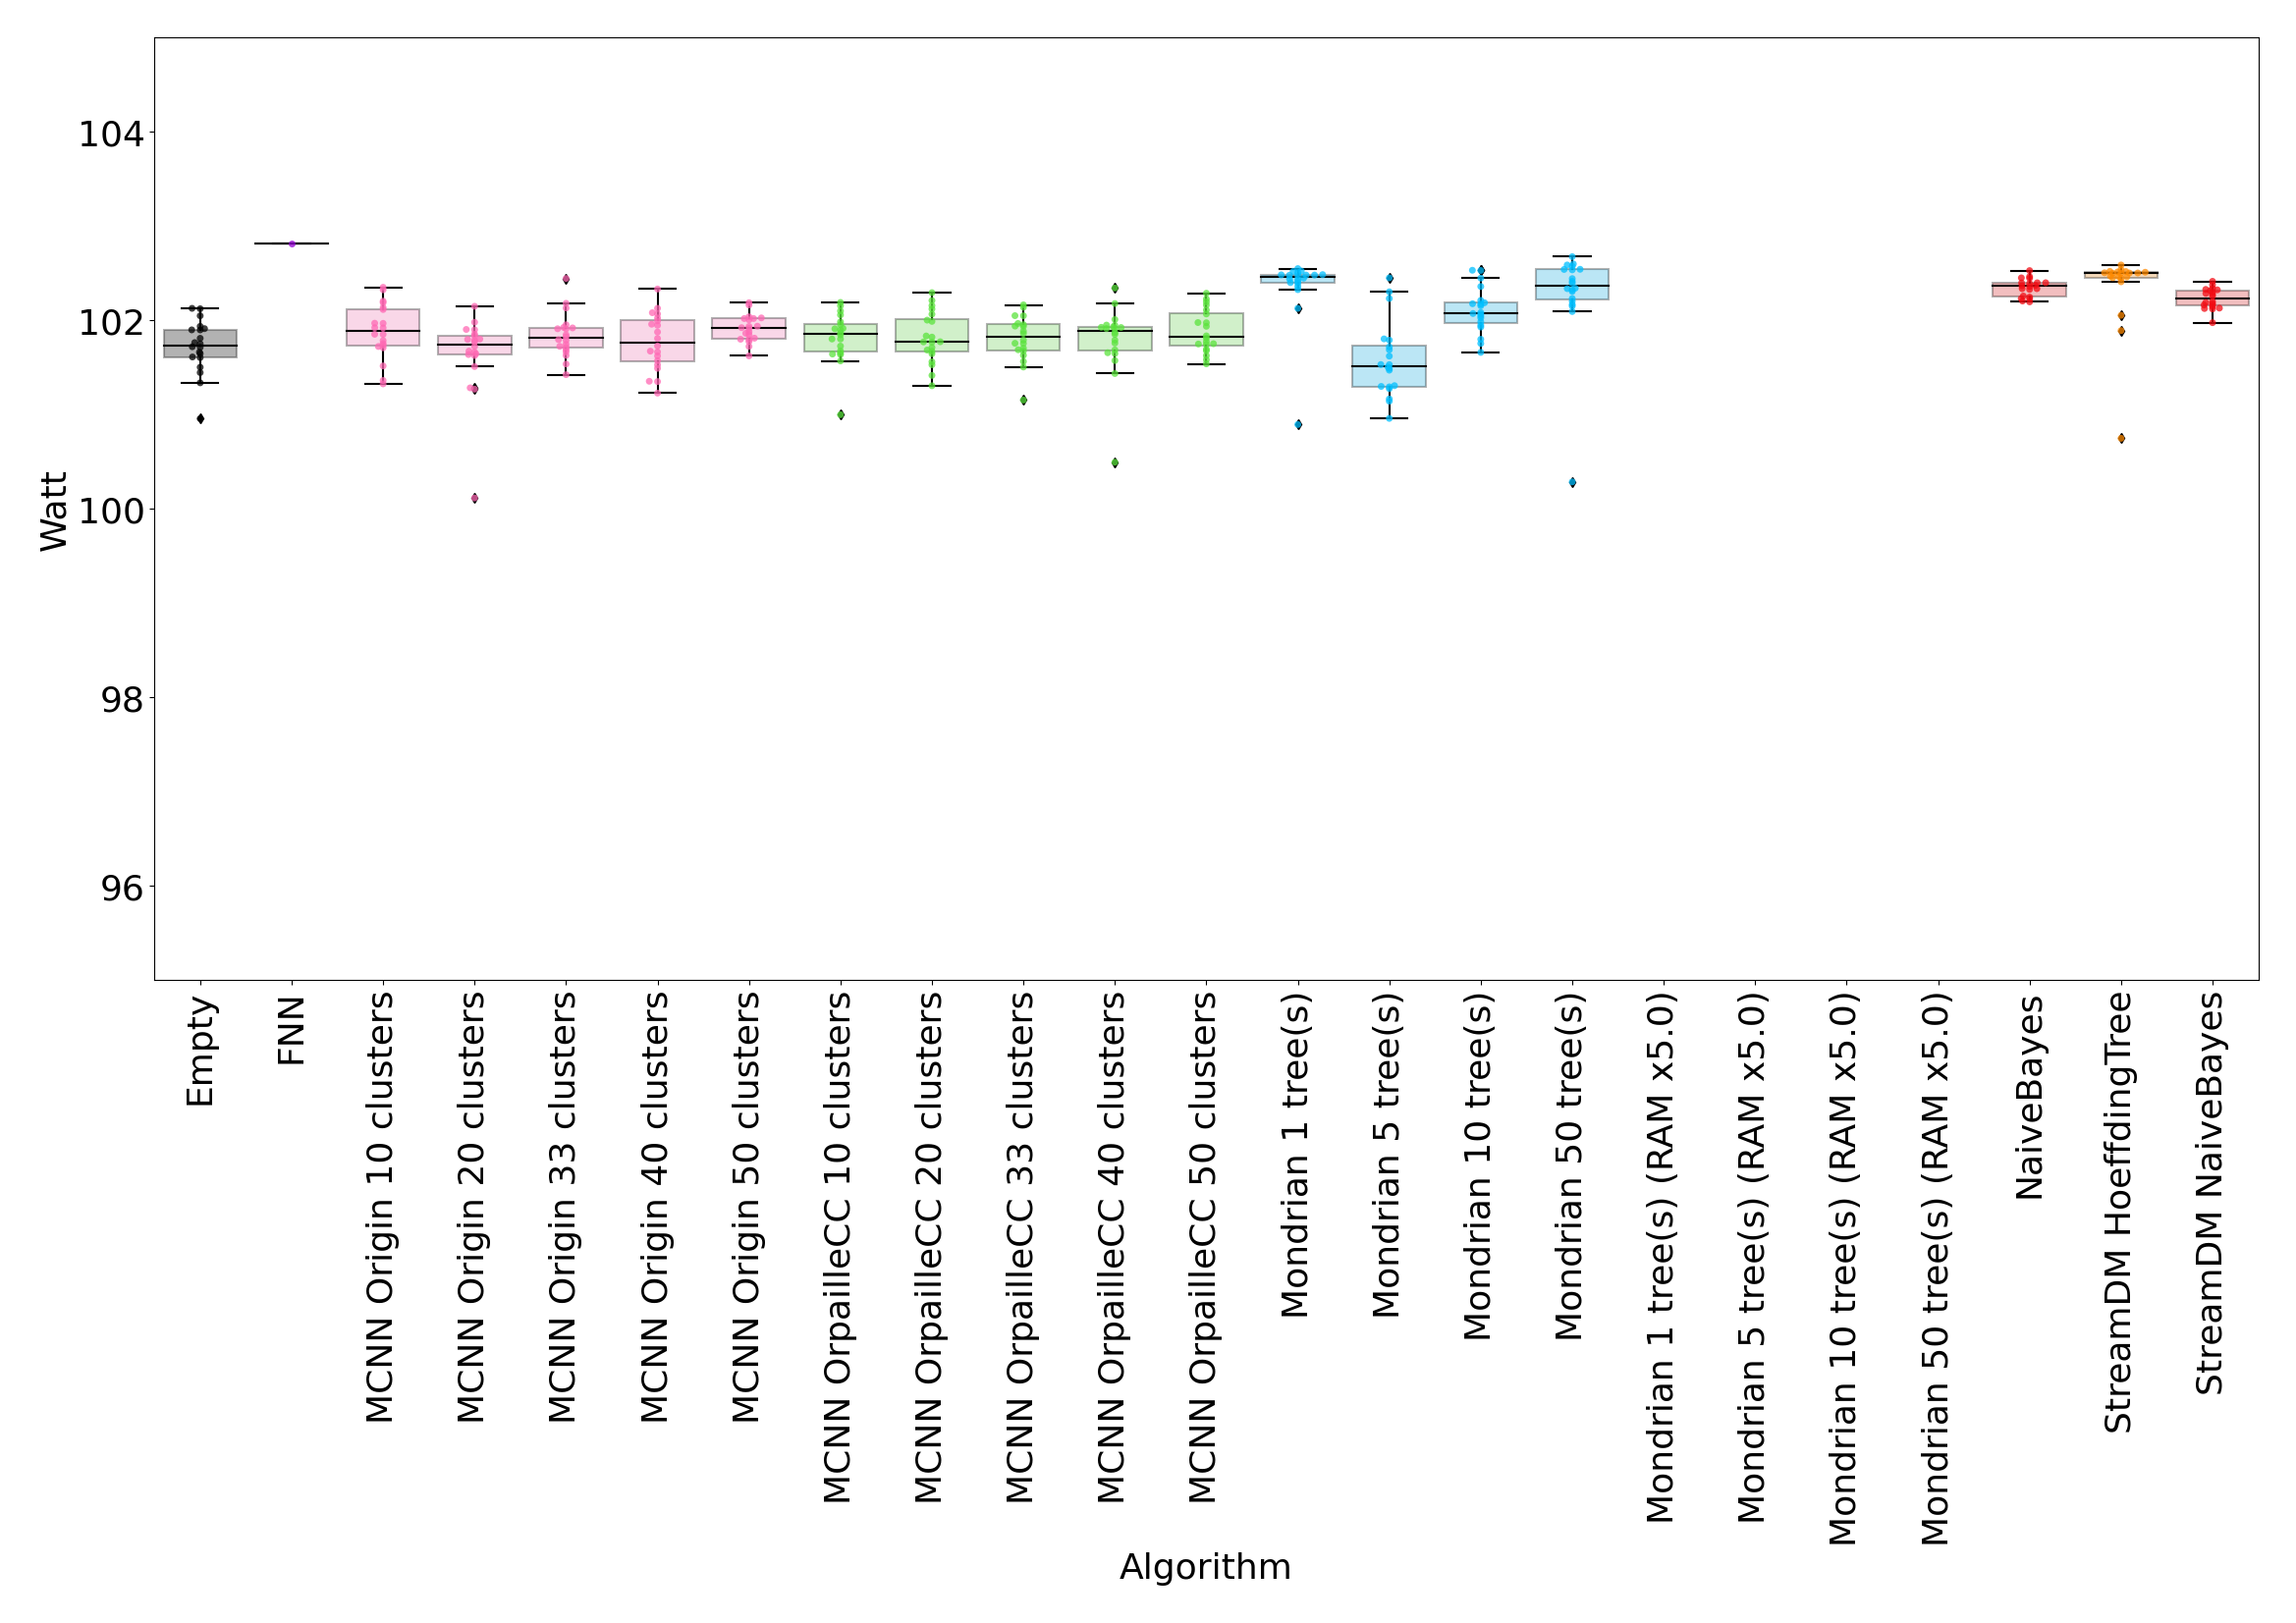
\includegraphics[width=\linewidth]{figures/results/drift_6_watt.png}
		\caption{\banosdataset with drift.}
		\label{fig:power-drift}
	\end{subfigure}\\
	\begin{subfigure}[t]{.49\linewidth}
		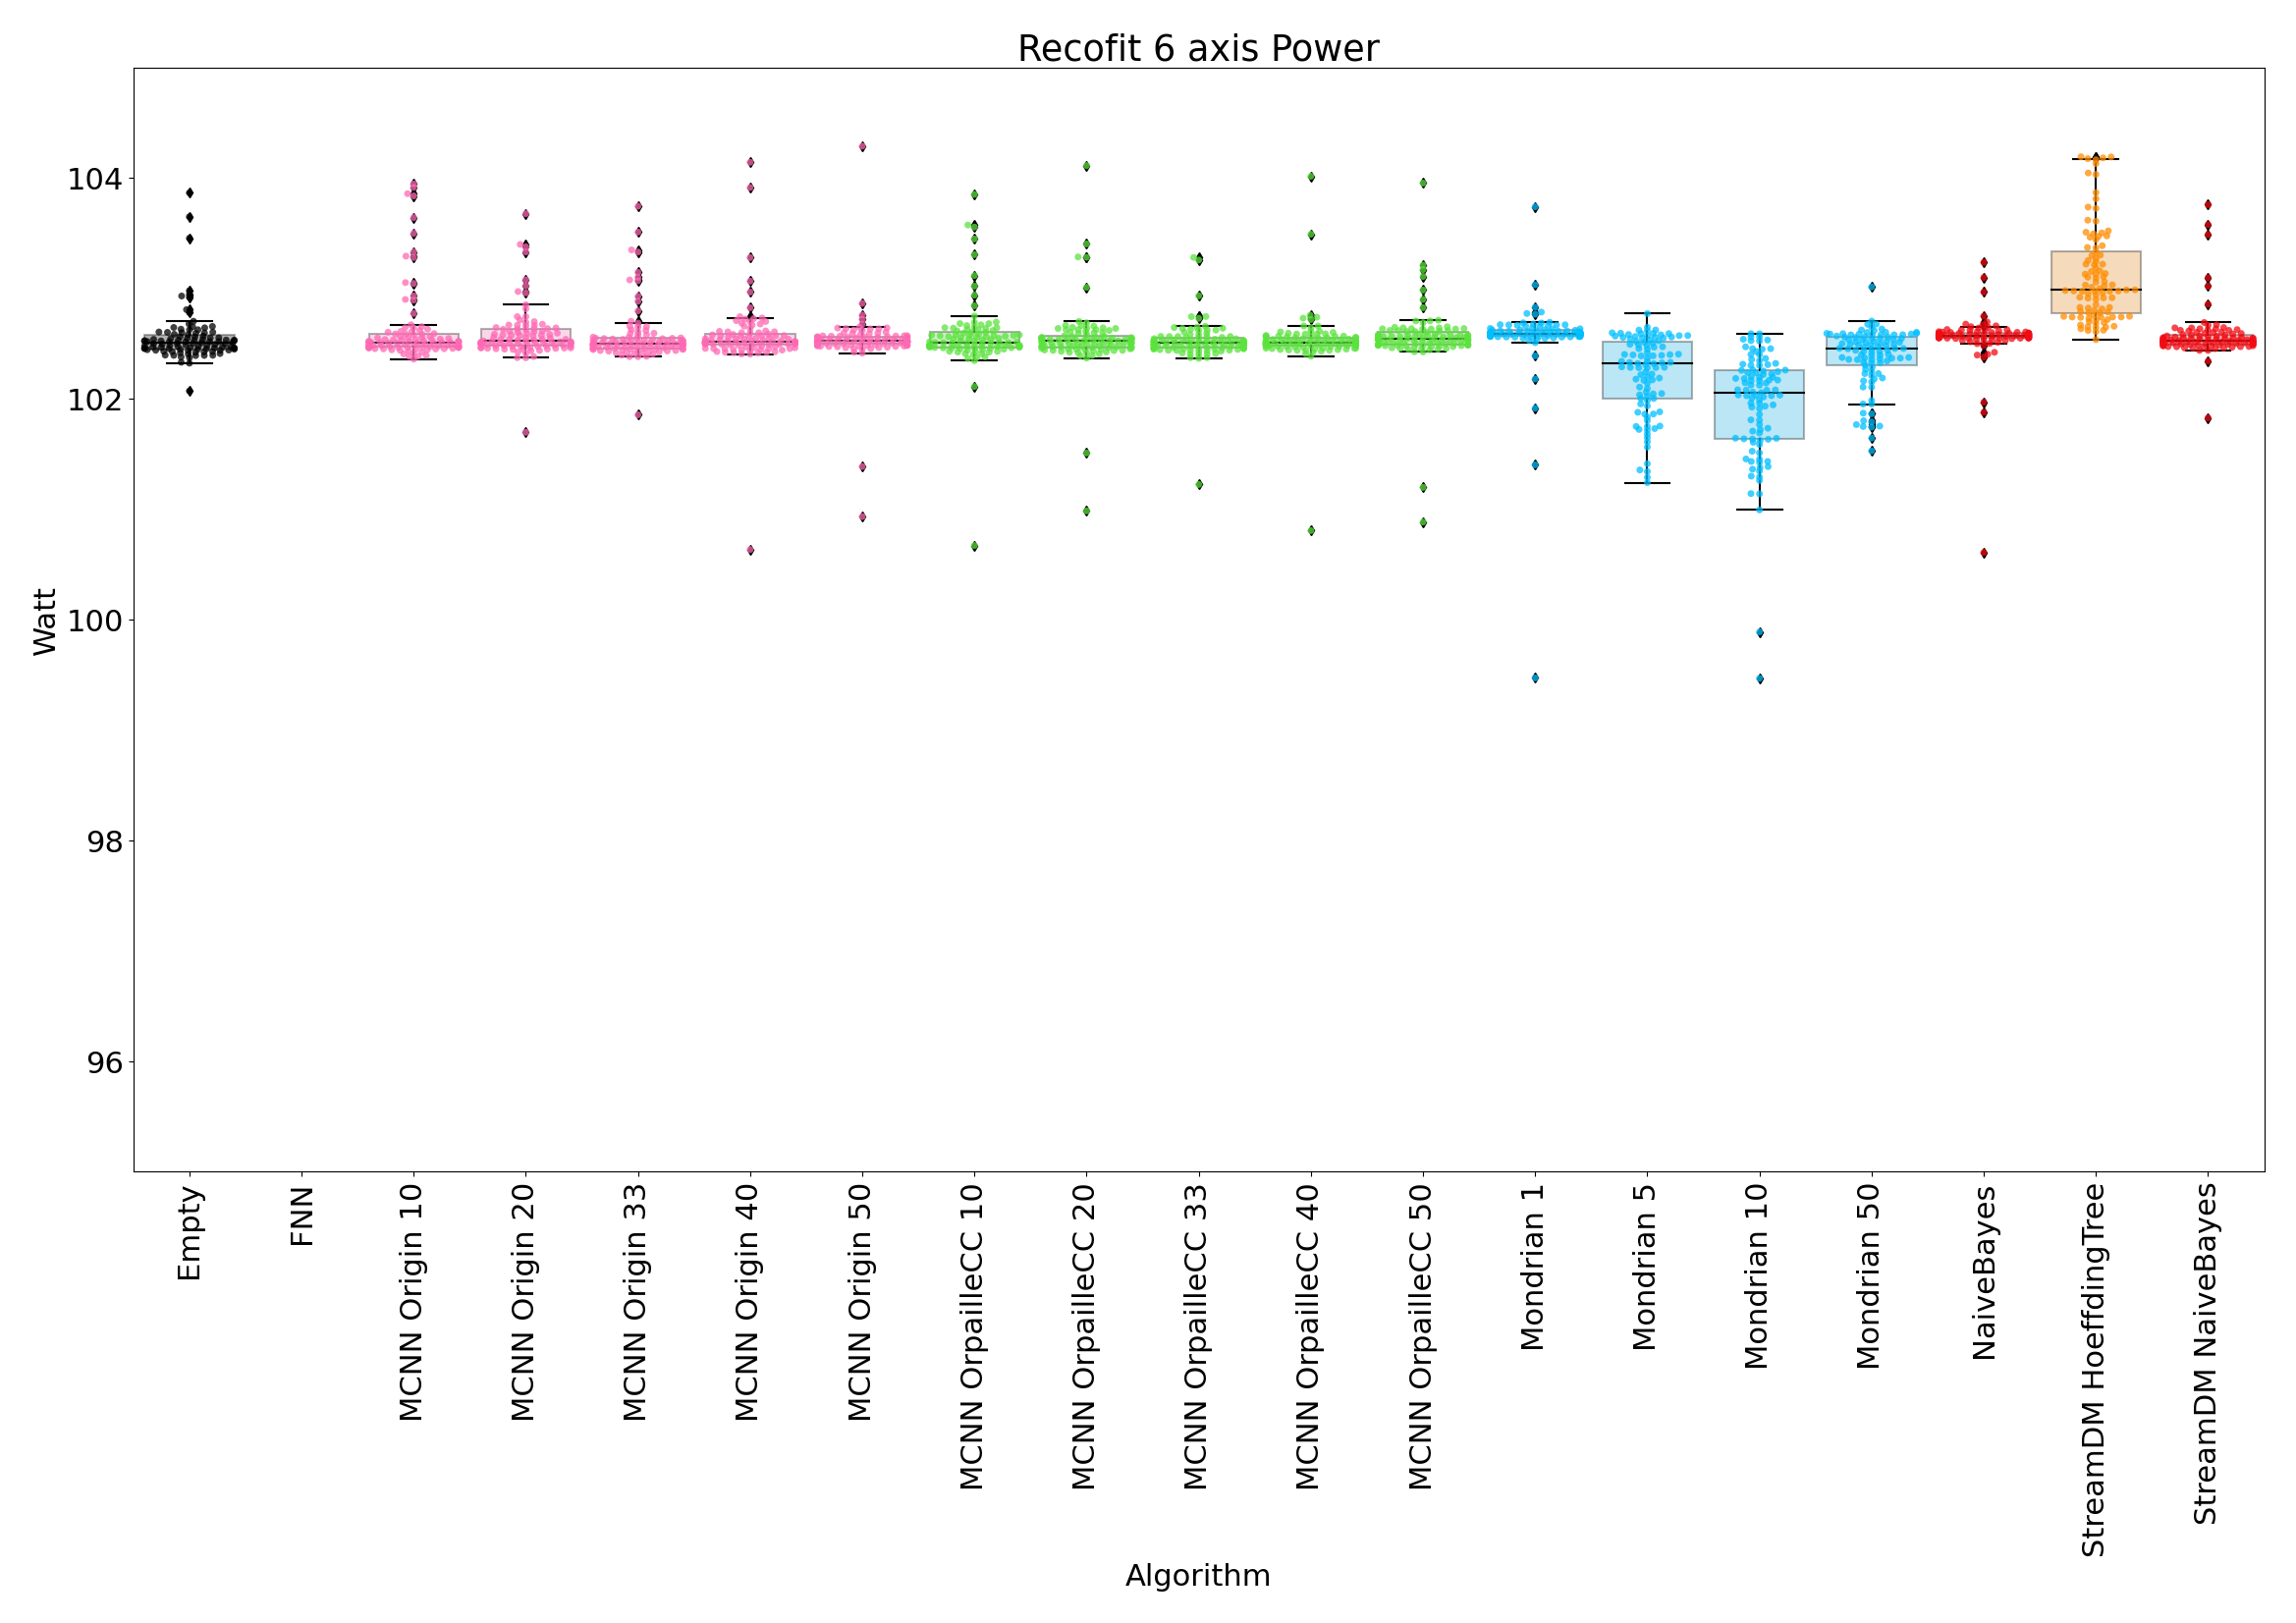
\includegraphics[width=\linewidth]{figures/results/recofit_6_watt.png}
		\caption{\recofitdataset}
		\label{fig:power-recofit}
	\end{subfigure}
	\hfill
	\begin{subfigure}[t]{.49\linewidth}
		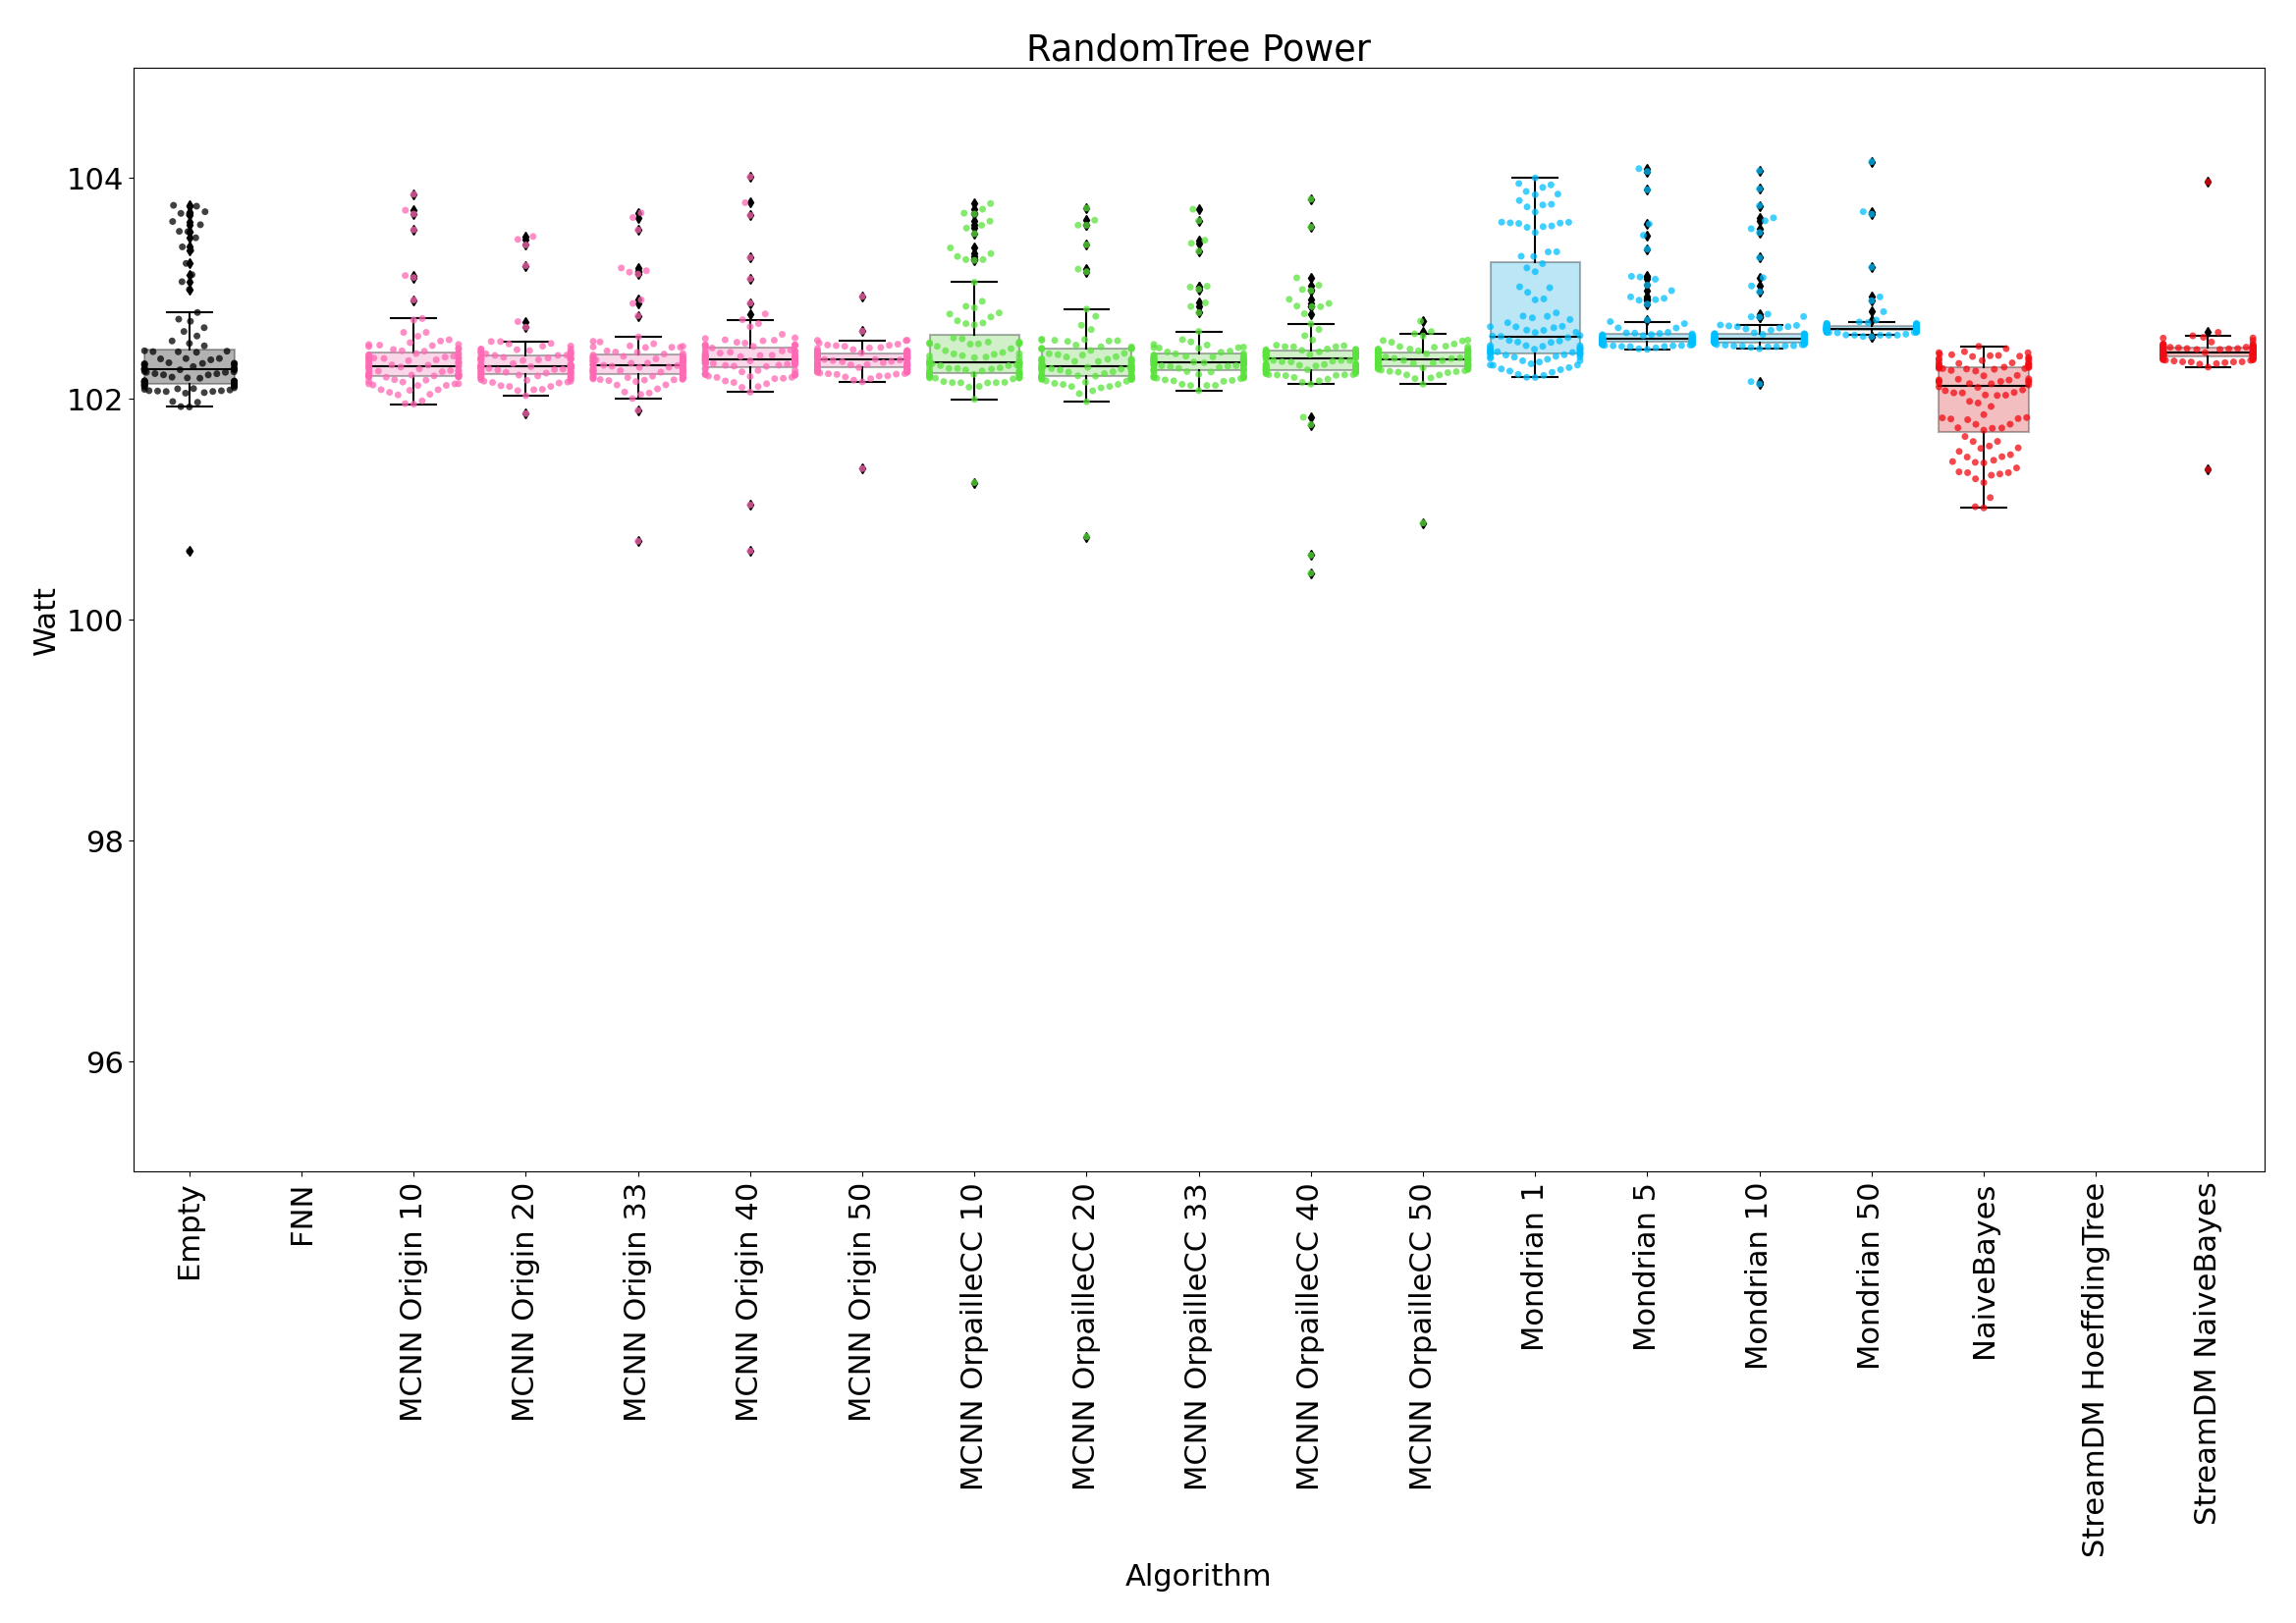
\includegraphics[width=\linewidth]{figures/results/dataset_3_watt.png}
		\caption{RandomTree}
		\label{fig:power-dataset_3}
	\end{subfigure}
	\caption{Power usage for four datasets.}
	\label{fig:power}
\end{figure*}
\subsection{Power}
\label{sec:result-power}
Figure~\ref{fig:power} shows the power usage of each classifier on four
datasets (results are similar for the other two datasets). All classifiers exhibit comparable power consumptions, close to
102~W. Figure~\ref{fig:power-drift} also
shows that the concept drift does not seem to influence power consumption.

This observation is explained by two factors. First, the benchmarking
platform was  working at minimal power. To ensure no disturbance by a
background process, we run the classifiers on an isolated cluster node with
eight cores. Therefore, the power difference on one core is not noticeable.

Another reason are the dataset sizes. Indeed, the slowest run is about
10 seconds with 50 Mondrian trees on \recofitdataset dataset. Such short
executions do not leave time for the CPU to switch P-states because it
barely warms a core. Further experiments would be required to check how 
our power consumption observations generalize to 
connected objects. 

\subsection{Runtime}

Figure~\ref{fig:runtime} shows the classifier runtimes for the two real
datasets. The \mondrianforest is the slowest classifier, in particular for 50
trees. The second slowest classifier is the \hoeffdingtree, with a runtime
comparable to the \mondrianforest with 10 trees. The \hoeffdingtree is followed
by the two \naivebayes implementations, which is not surprising since
\naivebayes classifiers are used in the leaves of the \hoeffdingtree. The \mcnn
classifiers are the fastest ones, with a runtime very close to the empty
classifier. Note that allocating more memory to the \mondrianforest
substantially increases runtime.

We observe that the runtime of StreamDM's \naivebayes is comparable to
OrpailleCC's. This suggests that the performance of the two libraries is
similar, which justifies our comparision of \hoeffdingtree and \mondrianforest.

\begin{figure*}
	\begin{subfigure}[t]{.49\linewidth}
		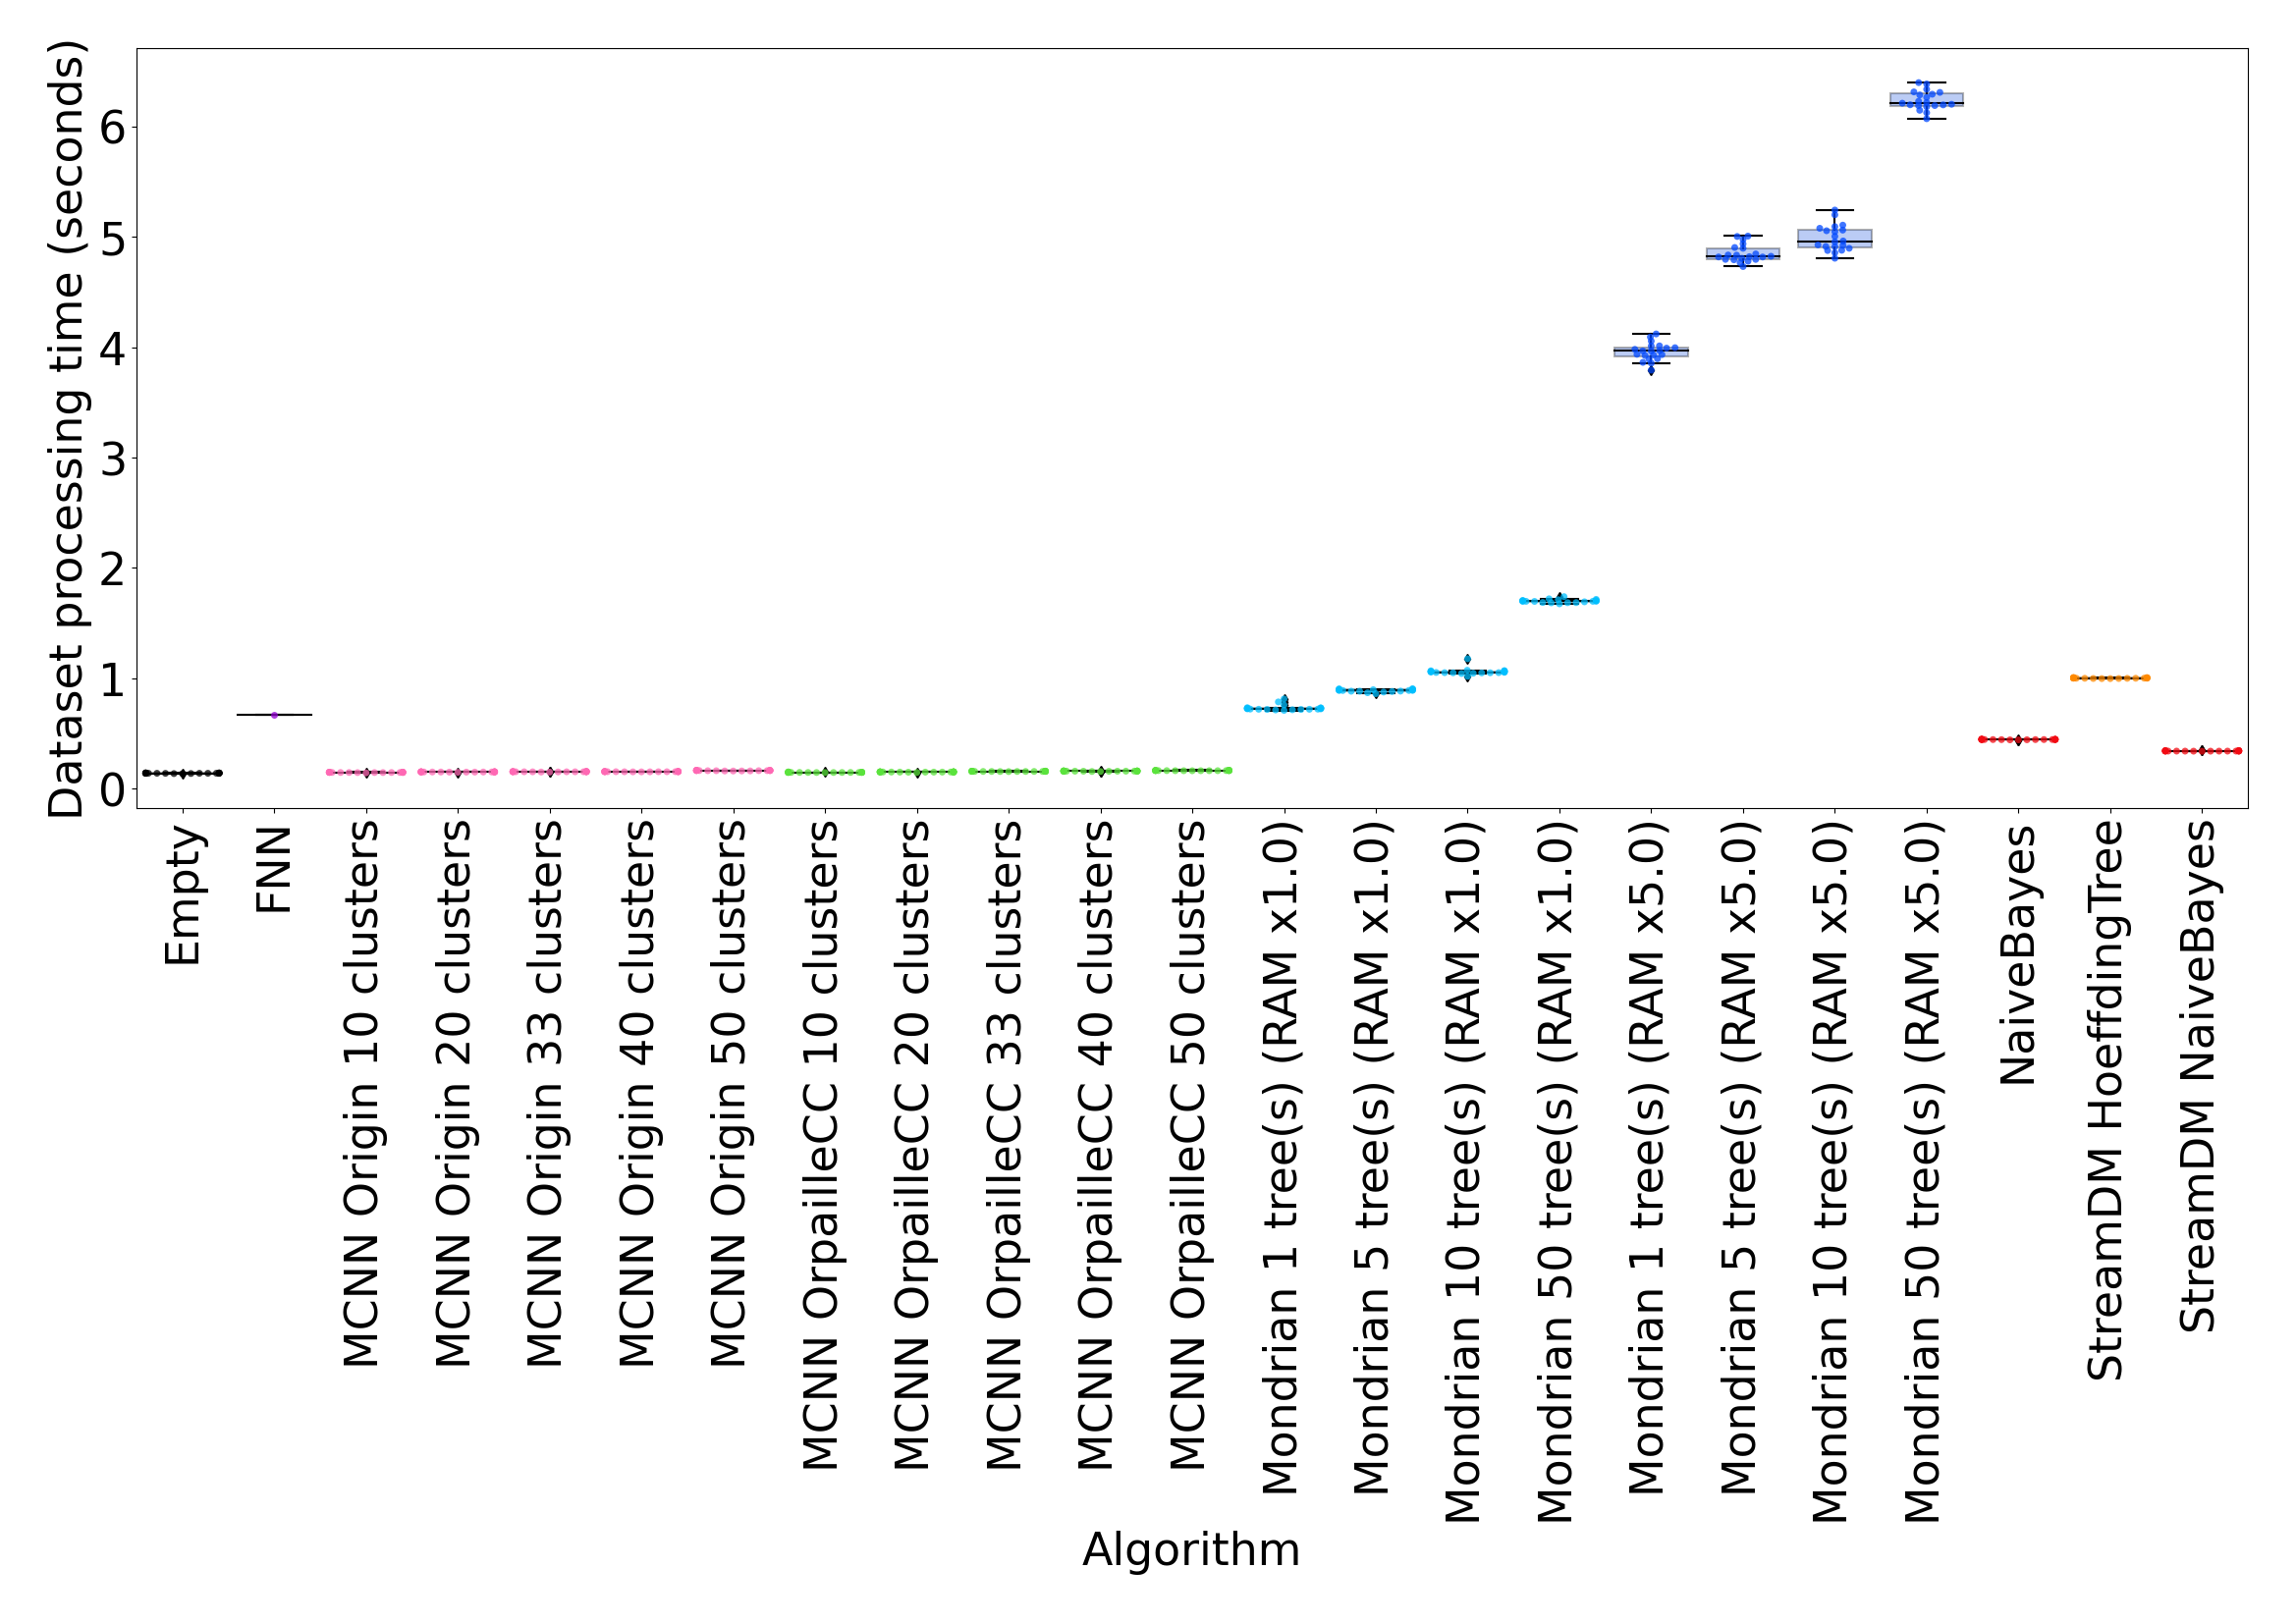
\includegraphics[width=\linewidth]{figures/results/banos_6_runtime.png}
		\caption{\banosdataset}
		\label{fig:runtime-banos}
	\end{subfigure}
	\hfill
	\begin{subfigure}[t]{.49\linewidth}
		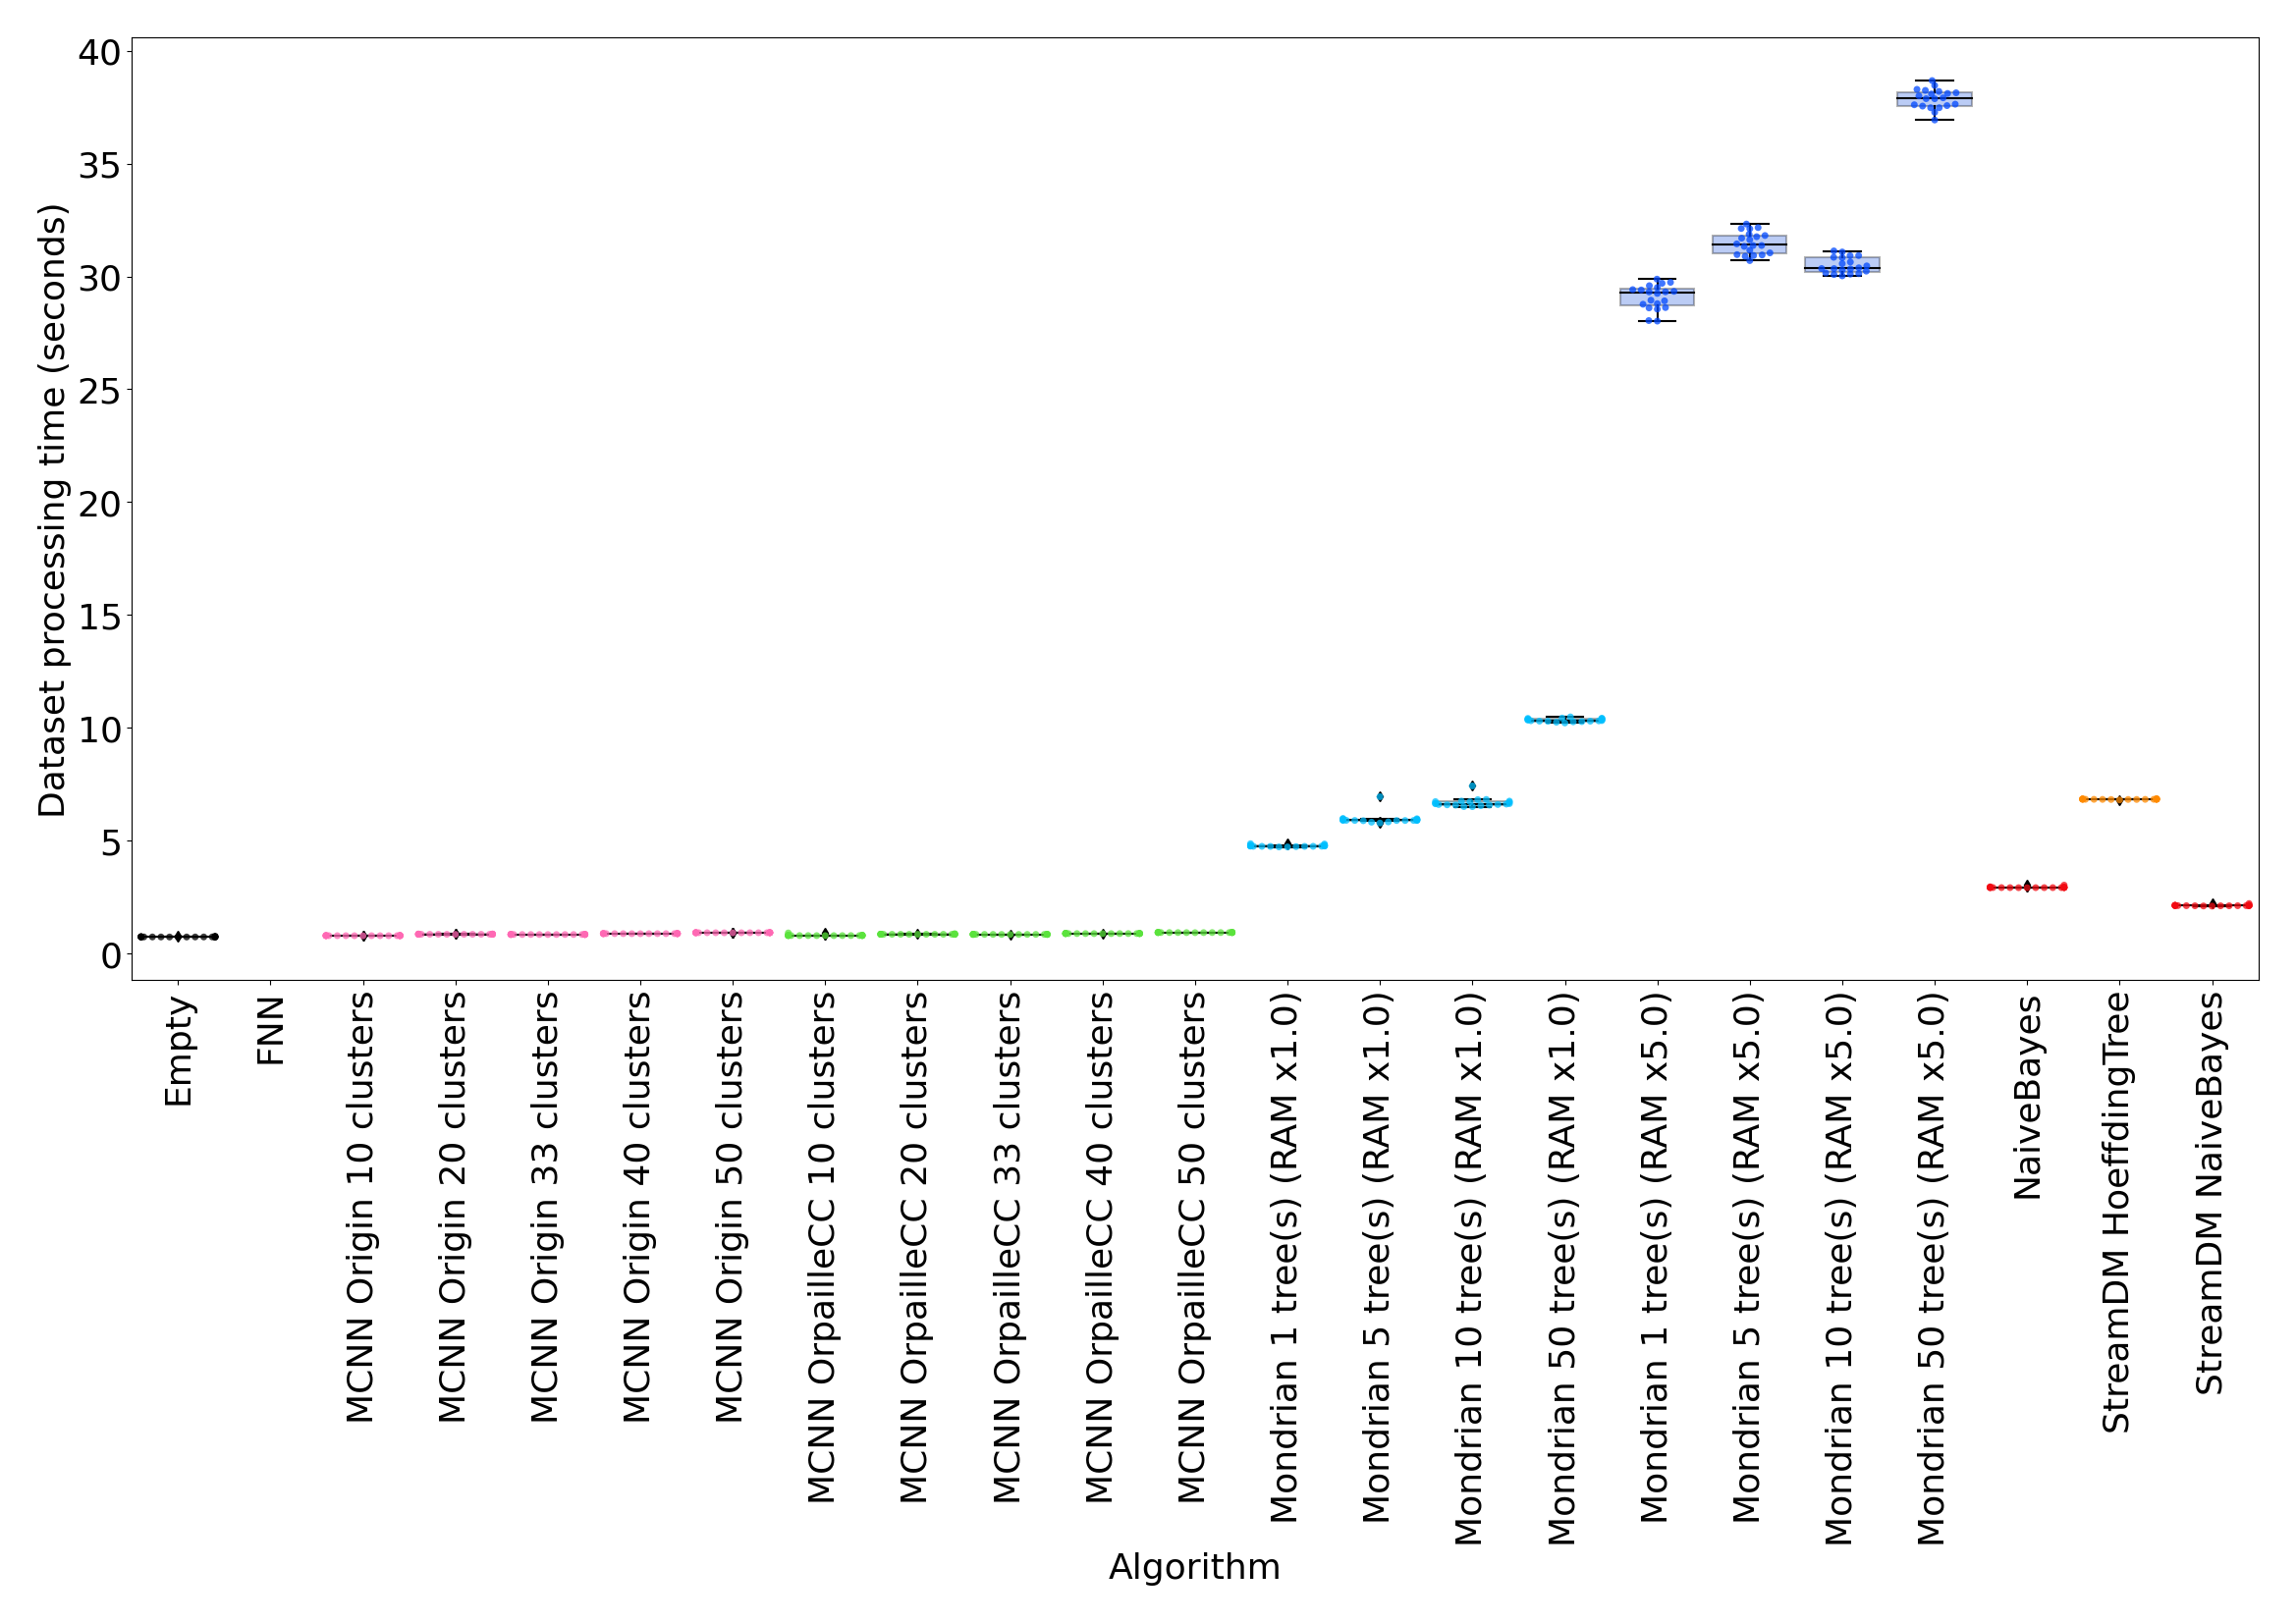
\includegraphics[width=\linewidth]{figures/results/recofit_6_runtime.png}
		\caption{\recofitdataset}
		\label{fig:runtime-recofit}
	\end{subfigure}
	\caption{Runtime with the two real datasets (20 repetitions).}
	\label{fig:runtime}
\end{figure*}

\subsection{Memory}
\label{sec:result-memory}
Figure~\ref{fig:memory} shows the evolution of the memory footprint for the
\banosdataset dataset. Results are similar for the other datasets and are
not reported for brevity. Since the  memory footprint of the \naivebayes
classifier was almost indistinguishable from the empty classifier, we used
the two \naivebayes as a baseline for the two libraries. This enables us to
remove the 1.2~MB overhead induced by StreamDM. The StreamDM memory
footprint matches the result in~\cite{StreamDM-CPP}, where the
\hoeffdingtree shows a memory footprint of 4.8MB.

We observe that the memory footprints of the \mondrianforest and the
\hoeffdingtree are substantially higher than for the other classifiers, which makes 
their deployment on connected objects challenging.
Overall, memory footprints are similar across datasets, due to the
fact that most algorithms follow a bounded memory policy or have a constant
space complexity.  The only exception is the \hoeffdingtree that constantly
selects new splits depending on new data points. The \mondrianforest has the
same behavior but the OrpailleCC implementation is memory-bounded, which
makes its memory footprint constant.
%  The concept drift does not
% increase the memory footprint of the \hoeffdingtree.

\begin{figure}
	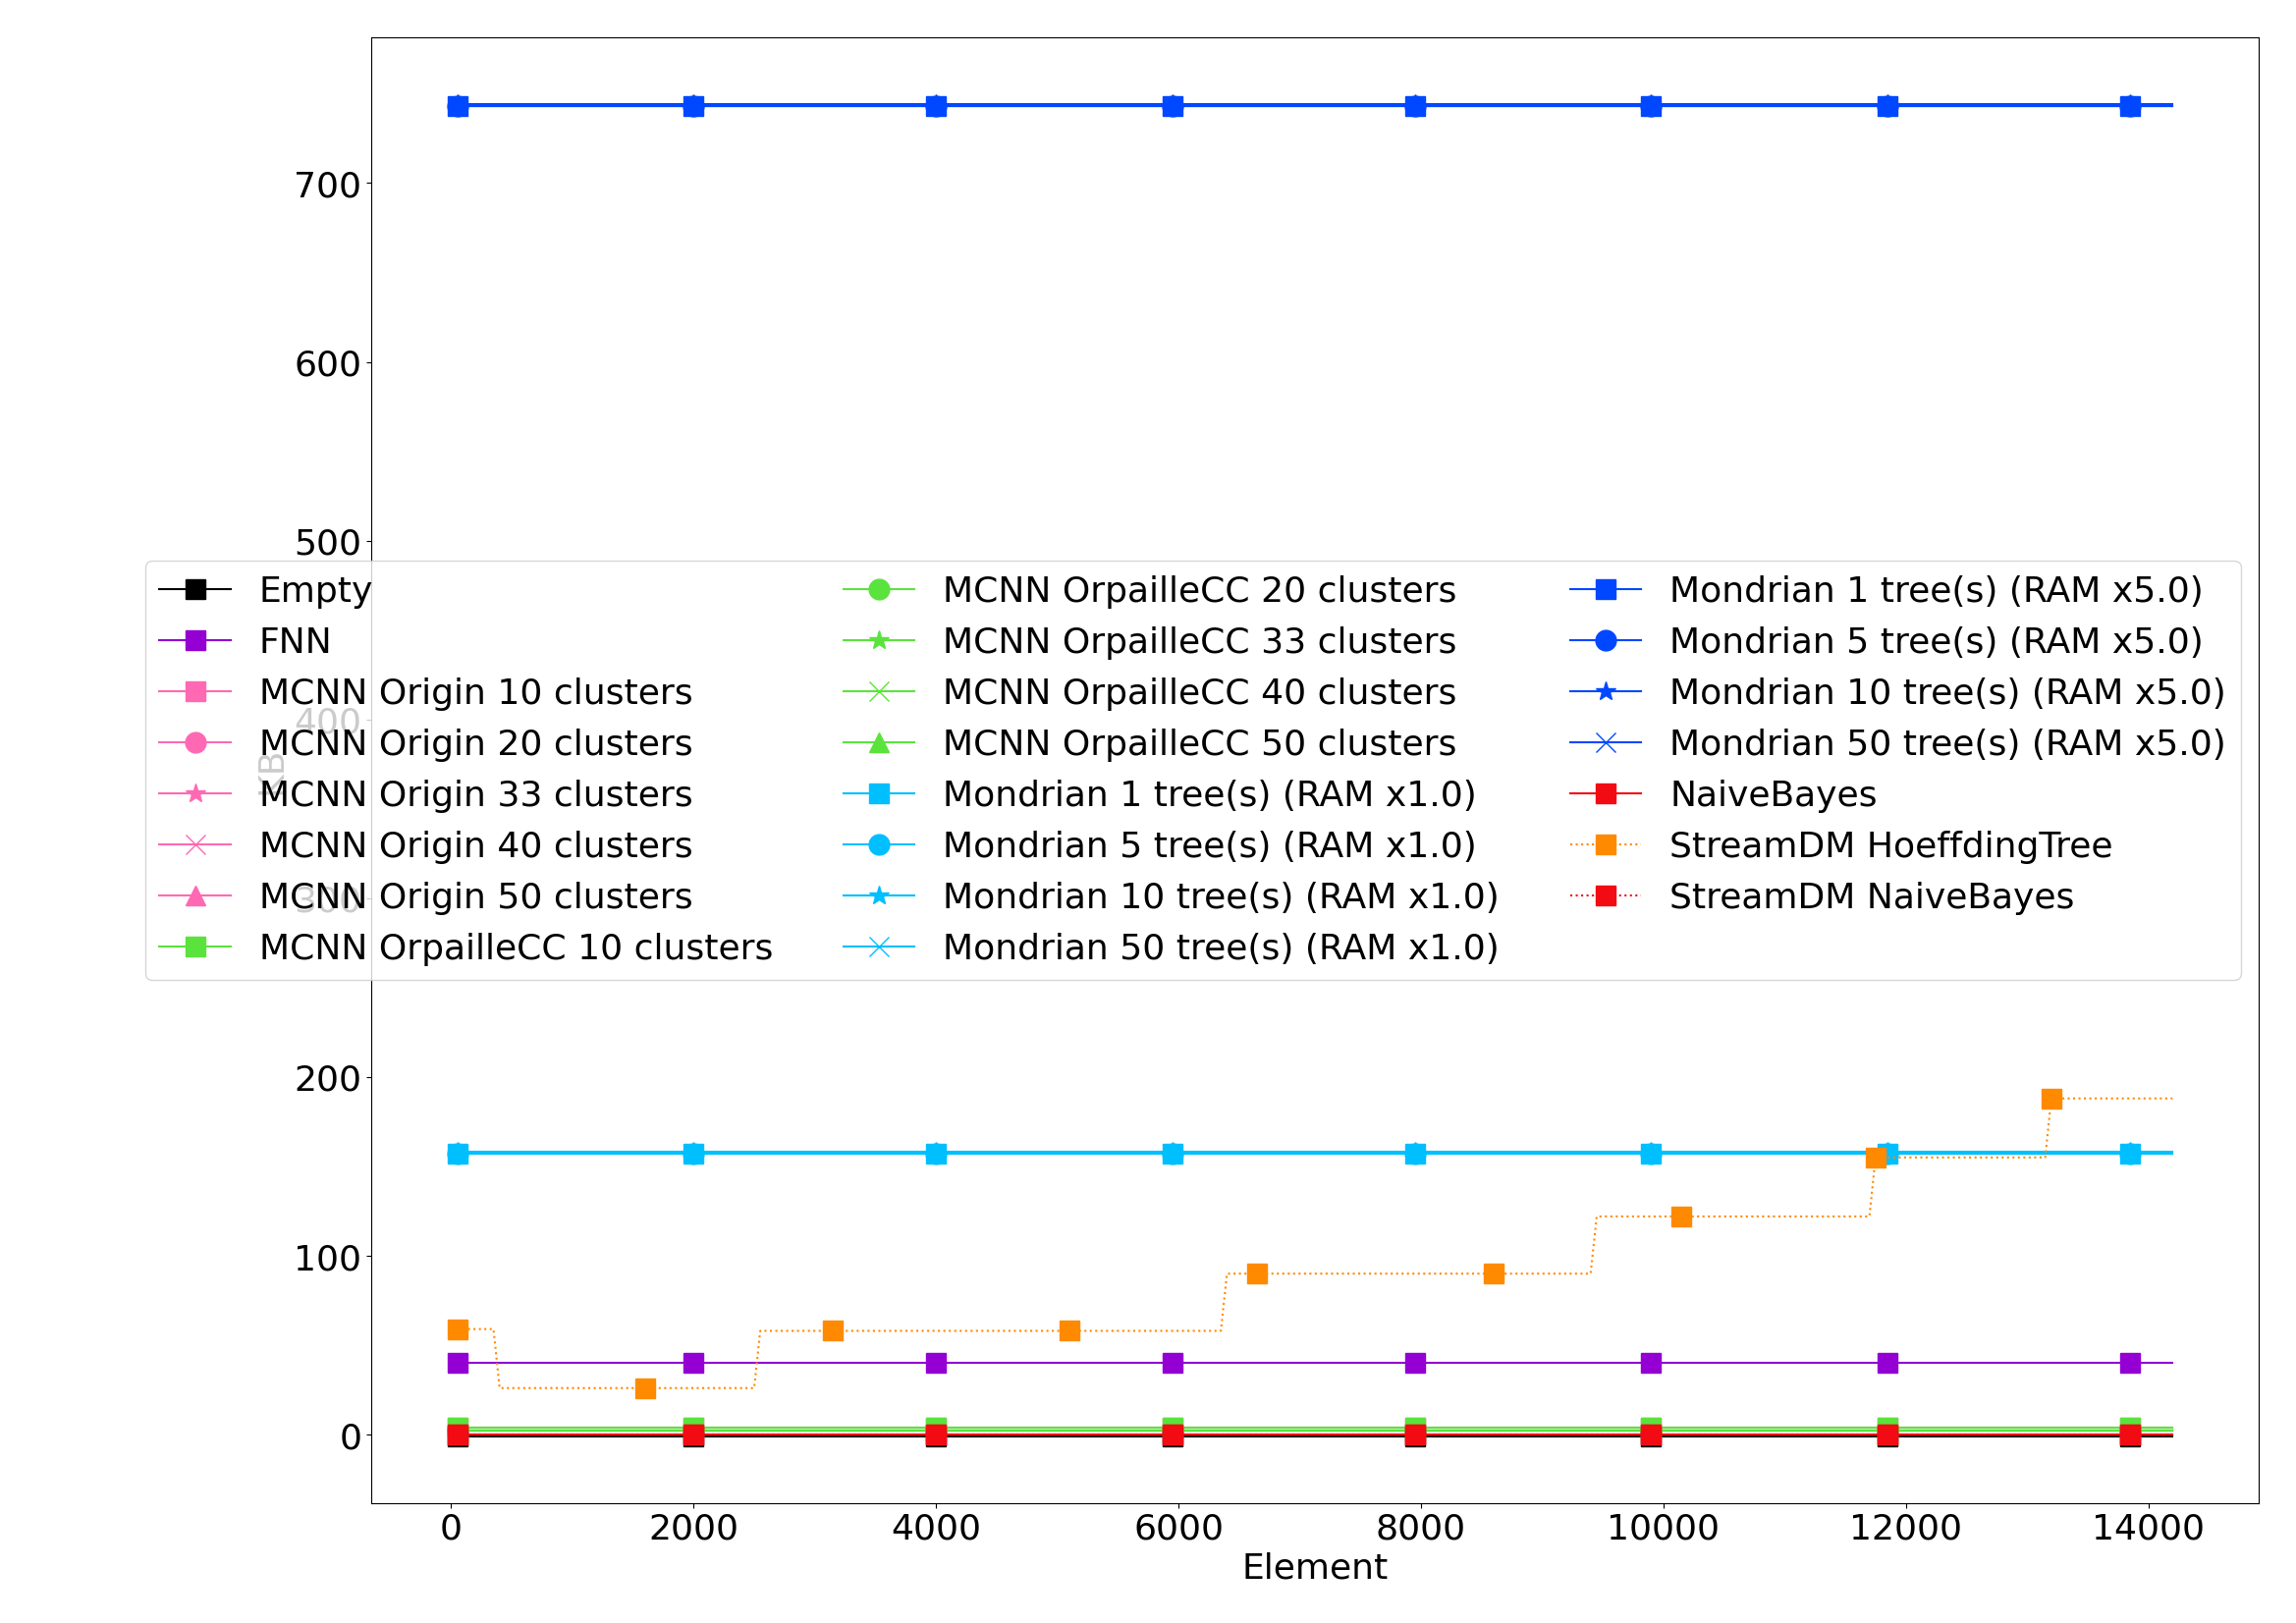
\includegraphics[width=\linewidth]{figures/results/banos_6_memory.png}
	\caption{Memory footprint of the classifiers relatively to the empty
	classifier, measured on the \banosdataset dataset. The memory footprint of the empty
	classifier is 3.439MB. The baselines are the two \naivebayes from OrpailleCC
		and StreamDM. They respectively have a memory footprint of 3.44OMB and
		4.743.}
	\label{fig:memory}
\end{figure}


\subsection{Hyperparameter tuning}

Figure~\ref{fig:mcnn-tuning-error} shows the impact of the error threshold
in the \mcnn classifiers with different cluster counts. The error
threshold of \mcnn has little impact on the classification performance. For
20 and 40 clusters, the best-performing threshold is either 2 or 4, meaning
that a cluster may do 2 or 4 errors before being split. For 10 clusters,
all error thresholds perform equally.

\begin{figure}
	 \begin{subfigure}[b]{0.49\textwidth}
		 \centering
		 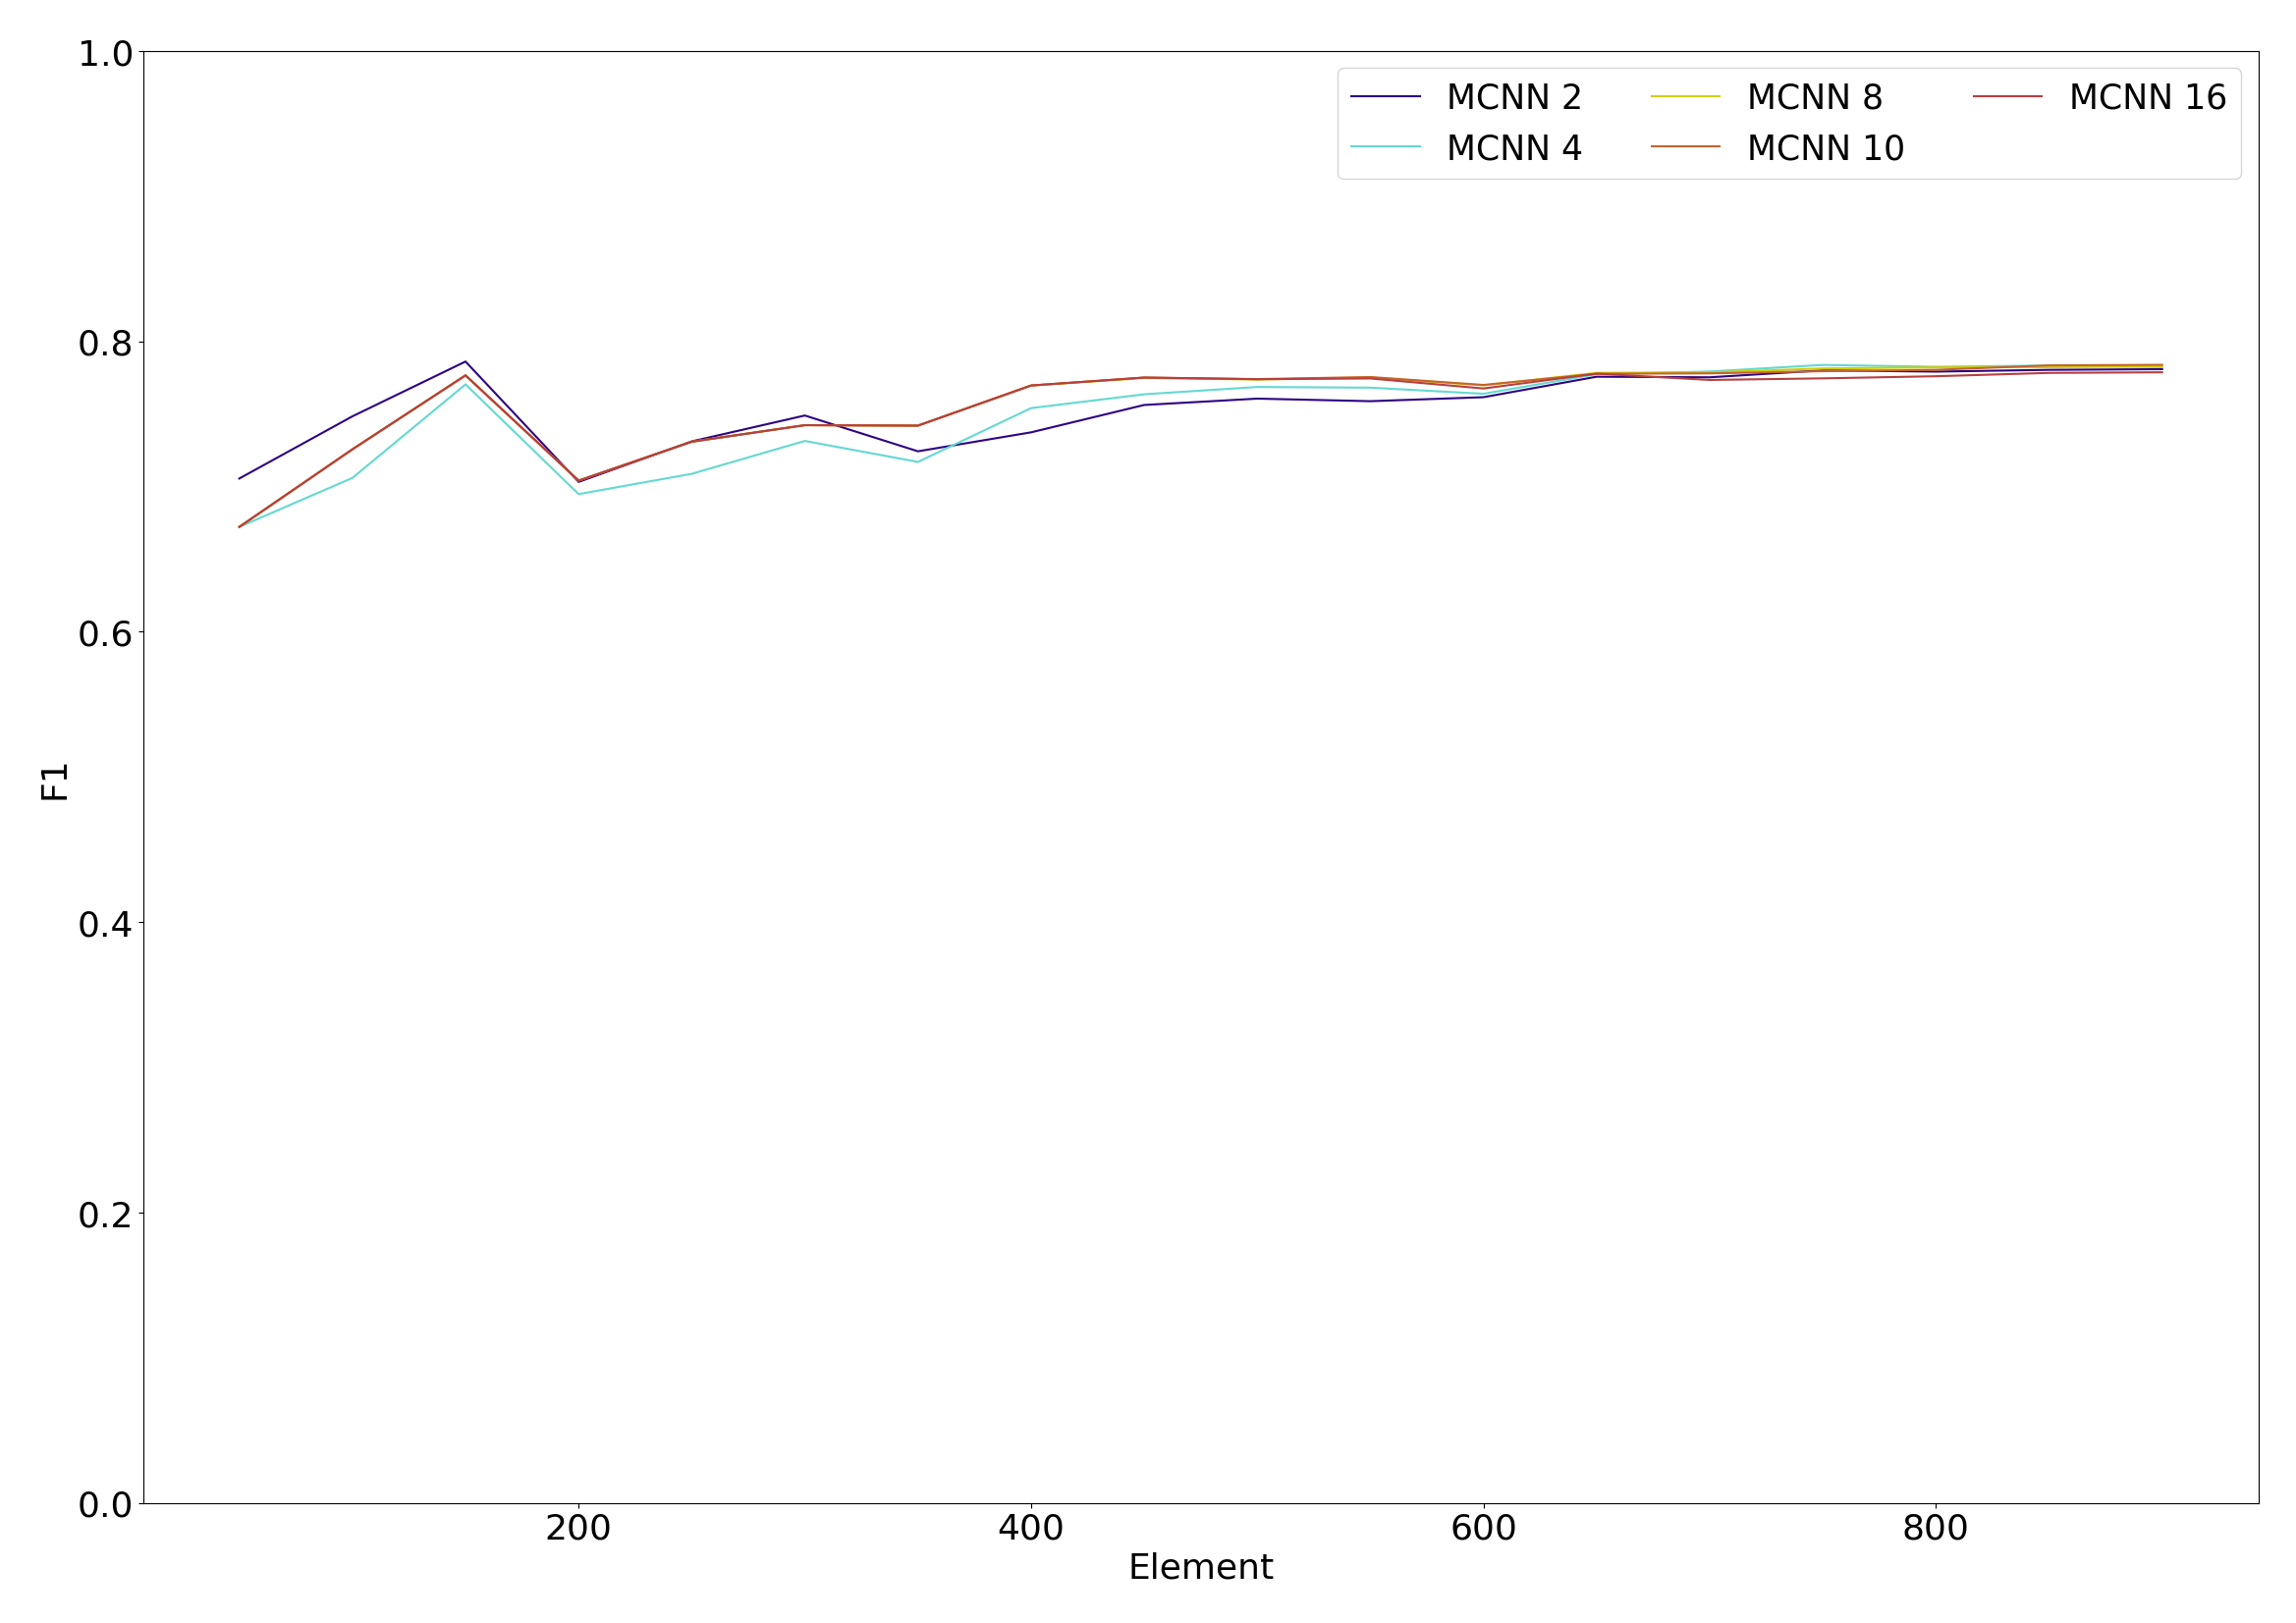
\includegraphics[width=\linewidth]{figures/calibration_mcnn_40.png}
		 \caption{40 clusters}
	 \end{subfigure}
	 \begin{subfigure}[b]{0.49\textwidth}
		 \centering
		 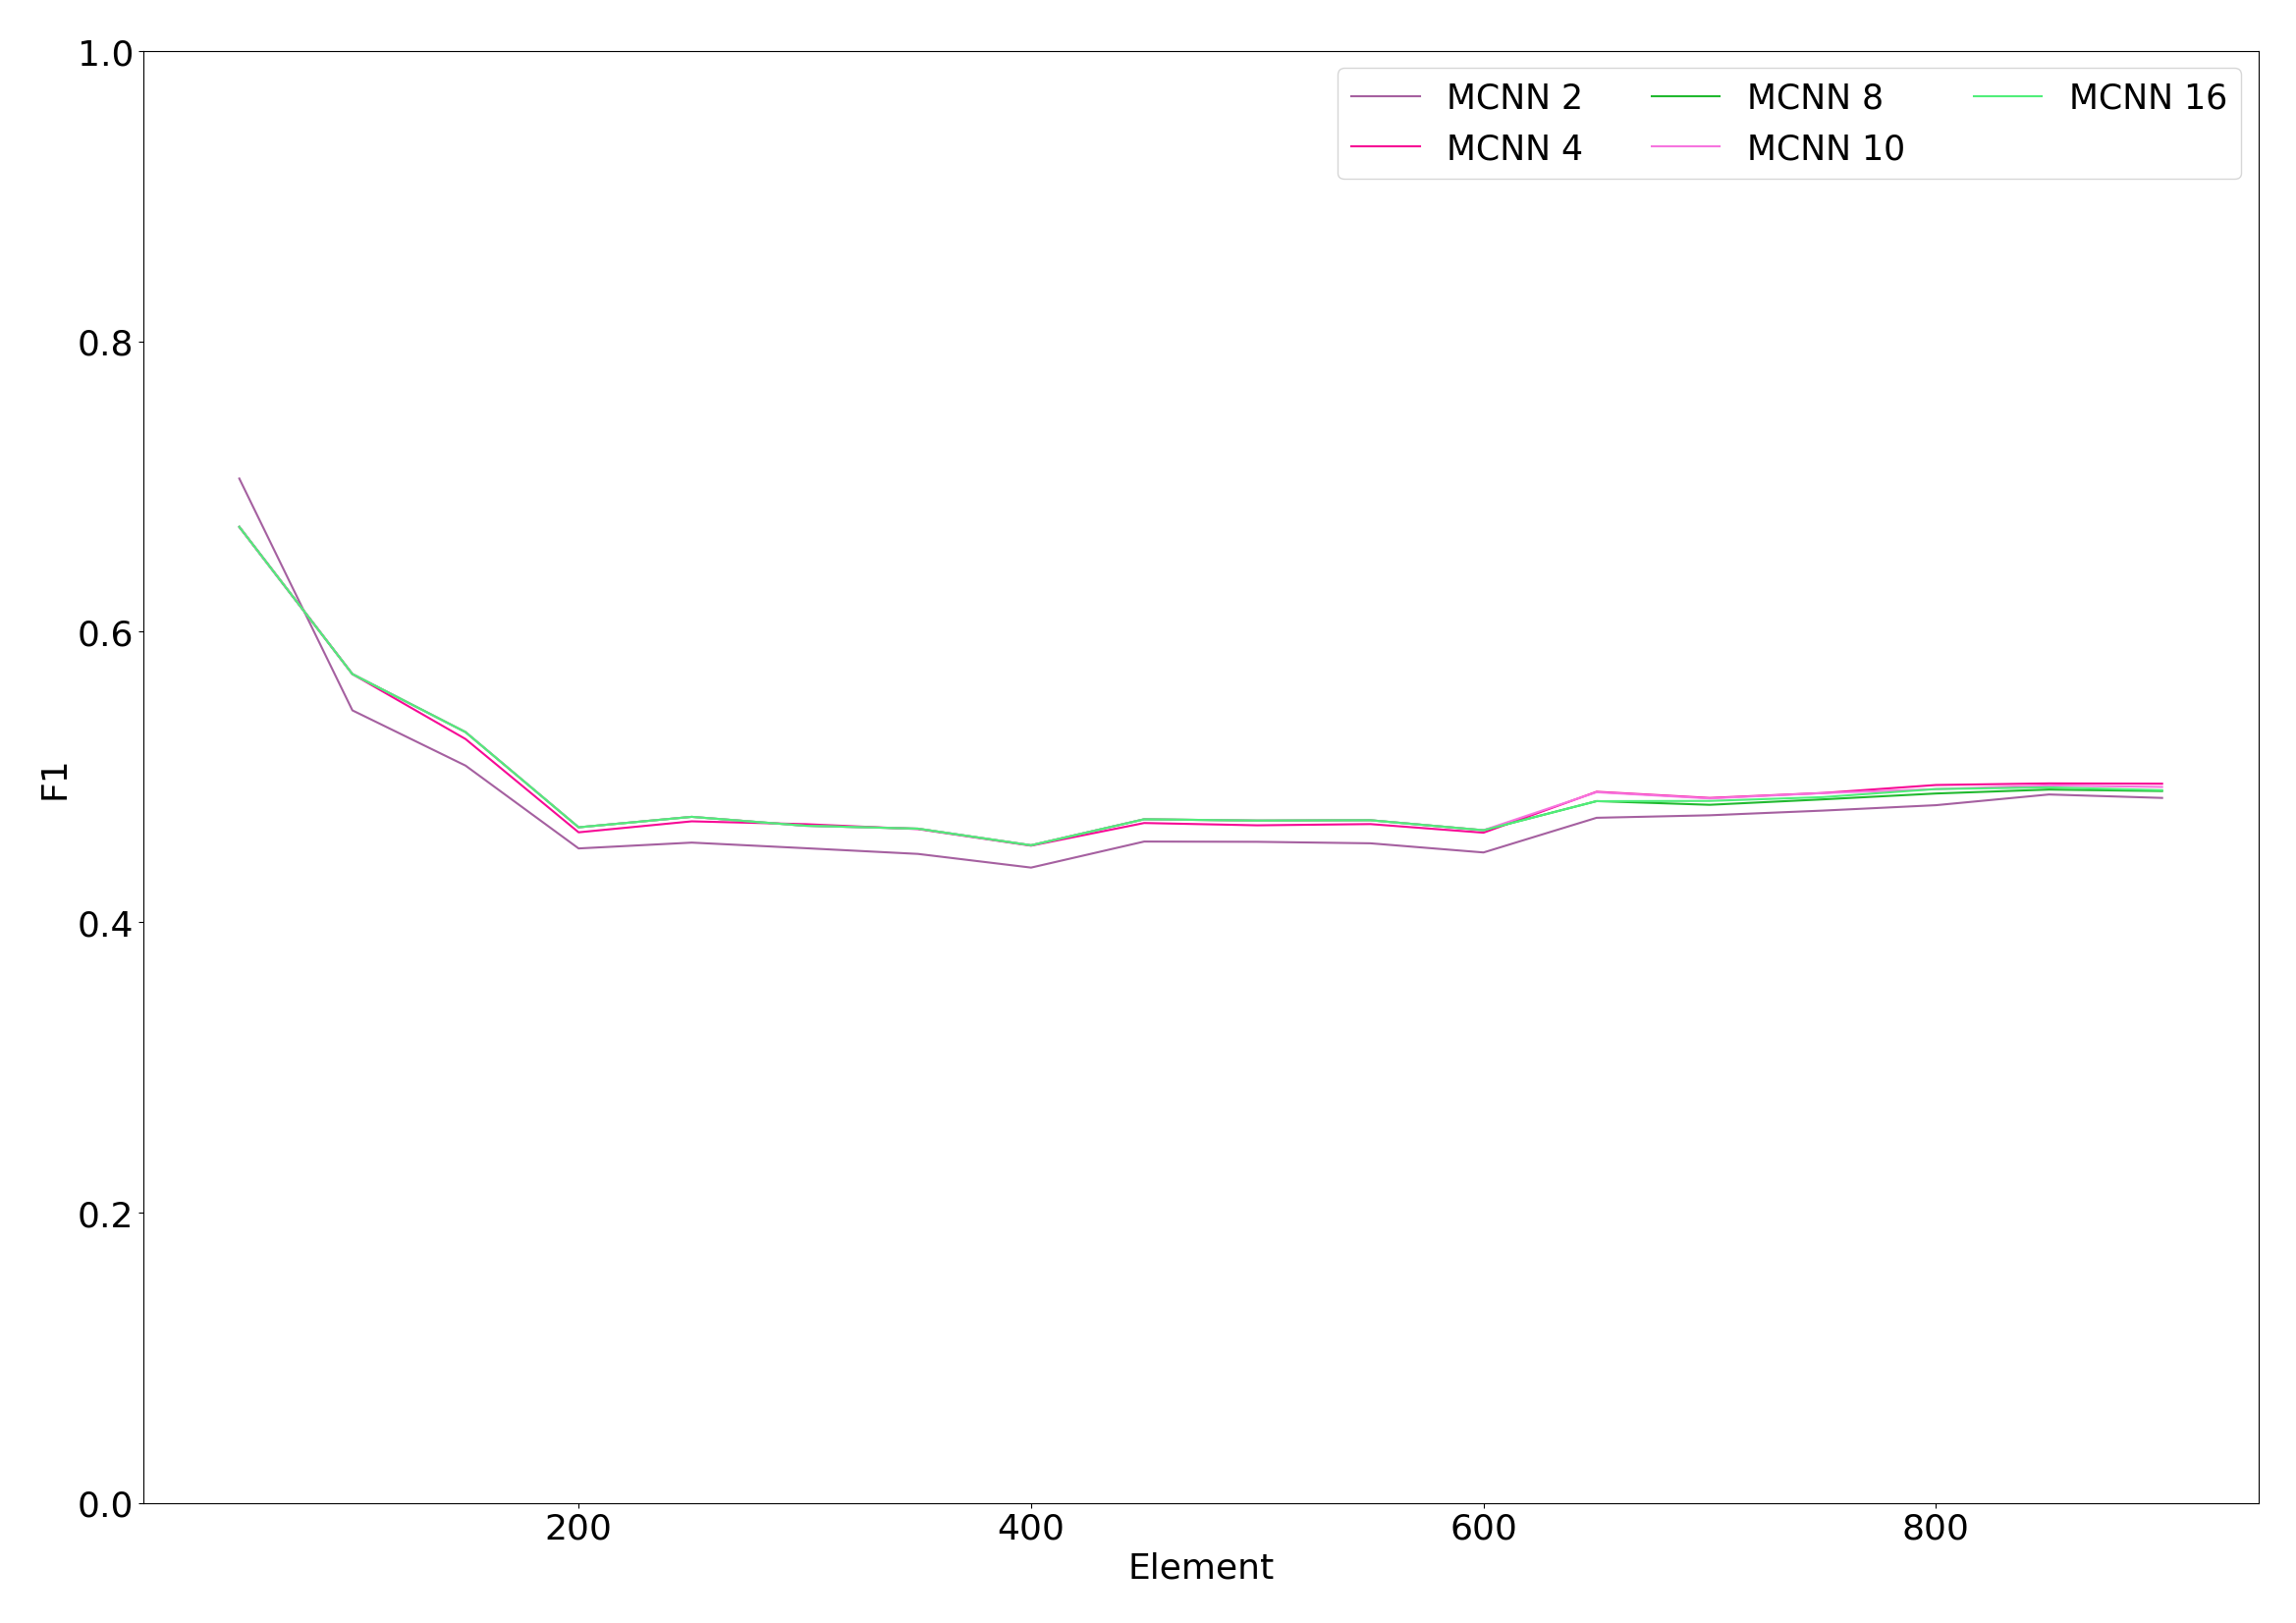
\includegraphics[width=\linewidth]{figures/calibration_mcnn_20.png}
		 \caption{20 clusters}
	 \end{subfigure}
	 \begin{subfigure}[b]{0.49\textwidth}
		 \centering
		 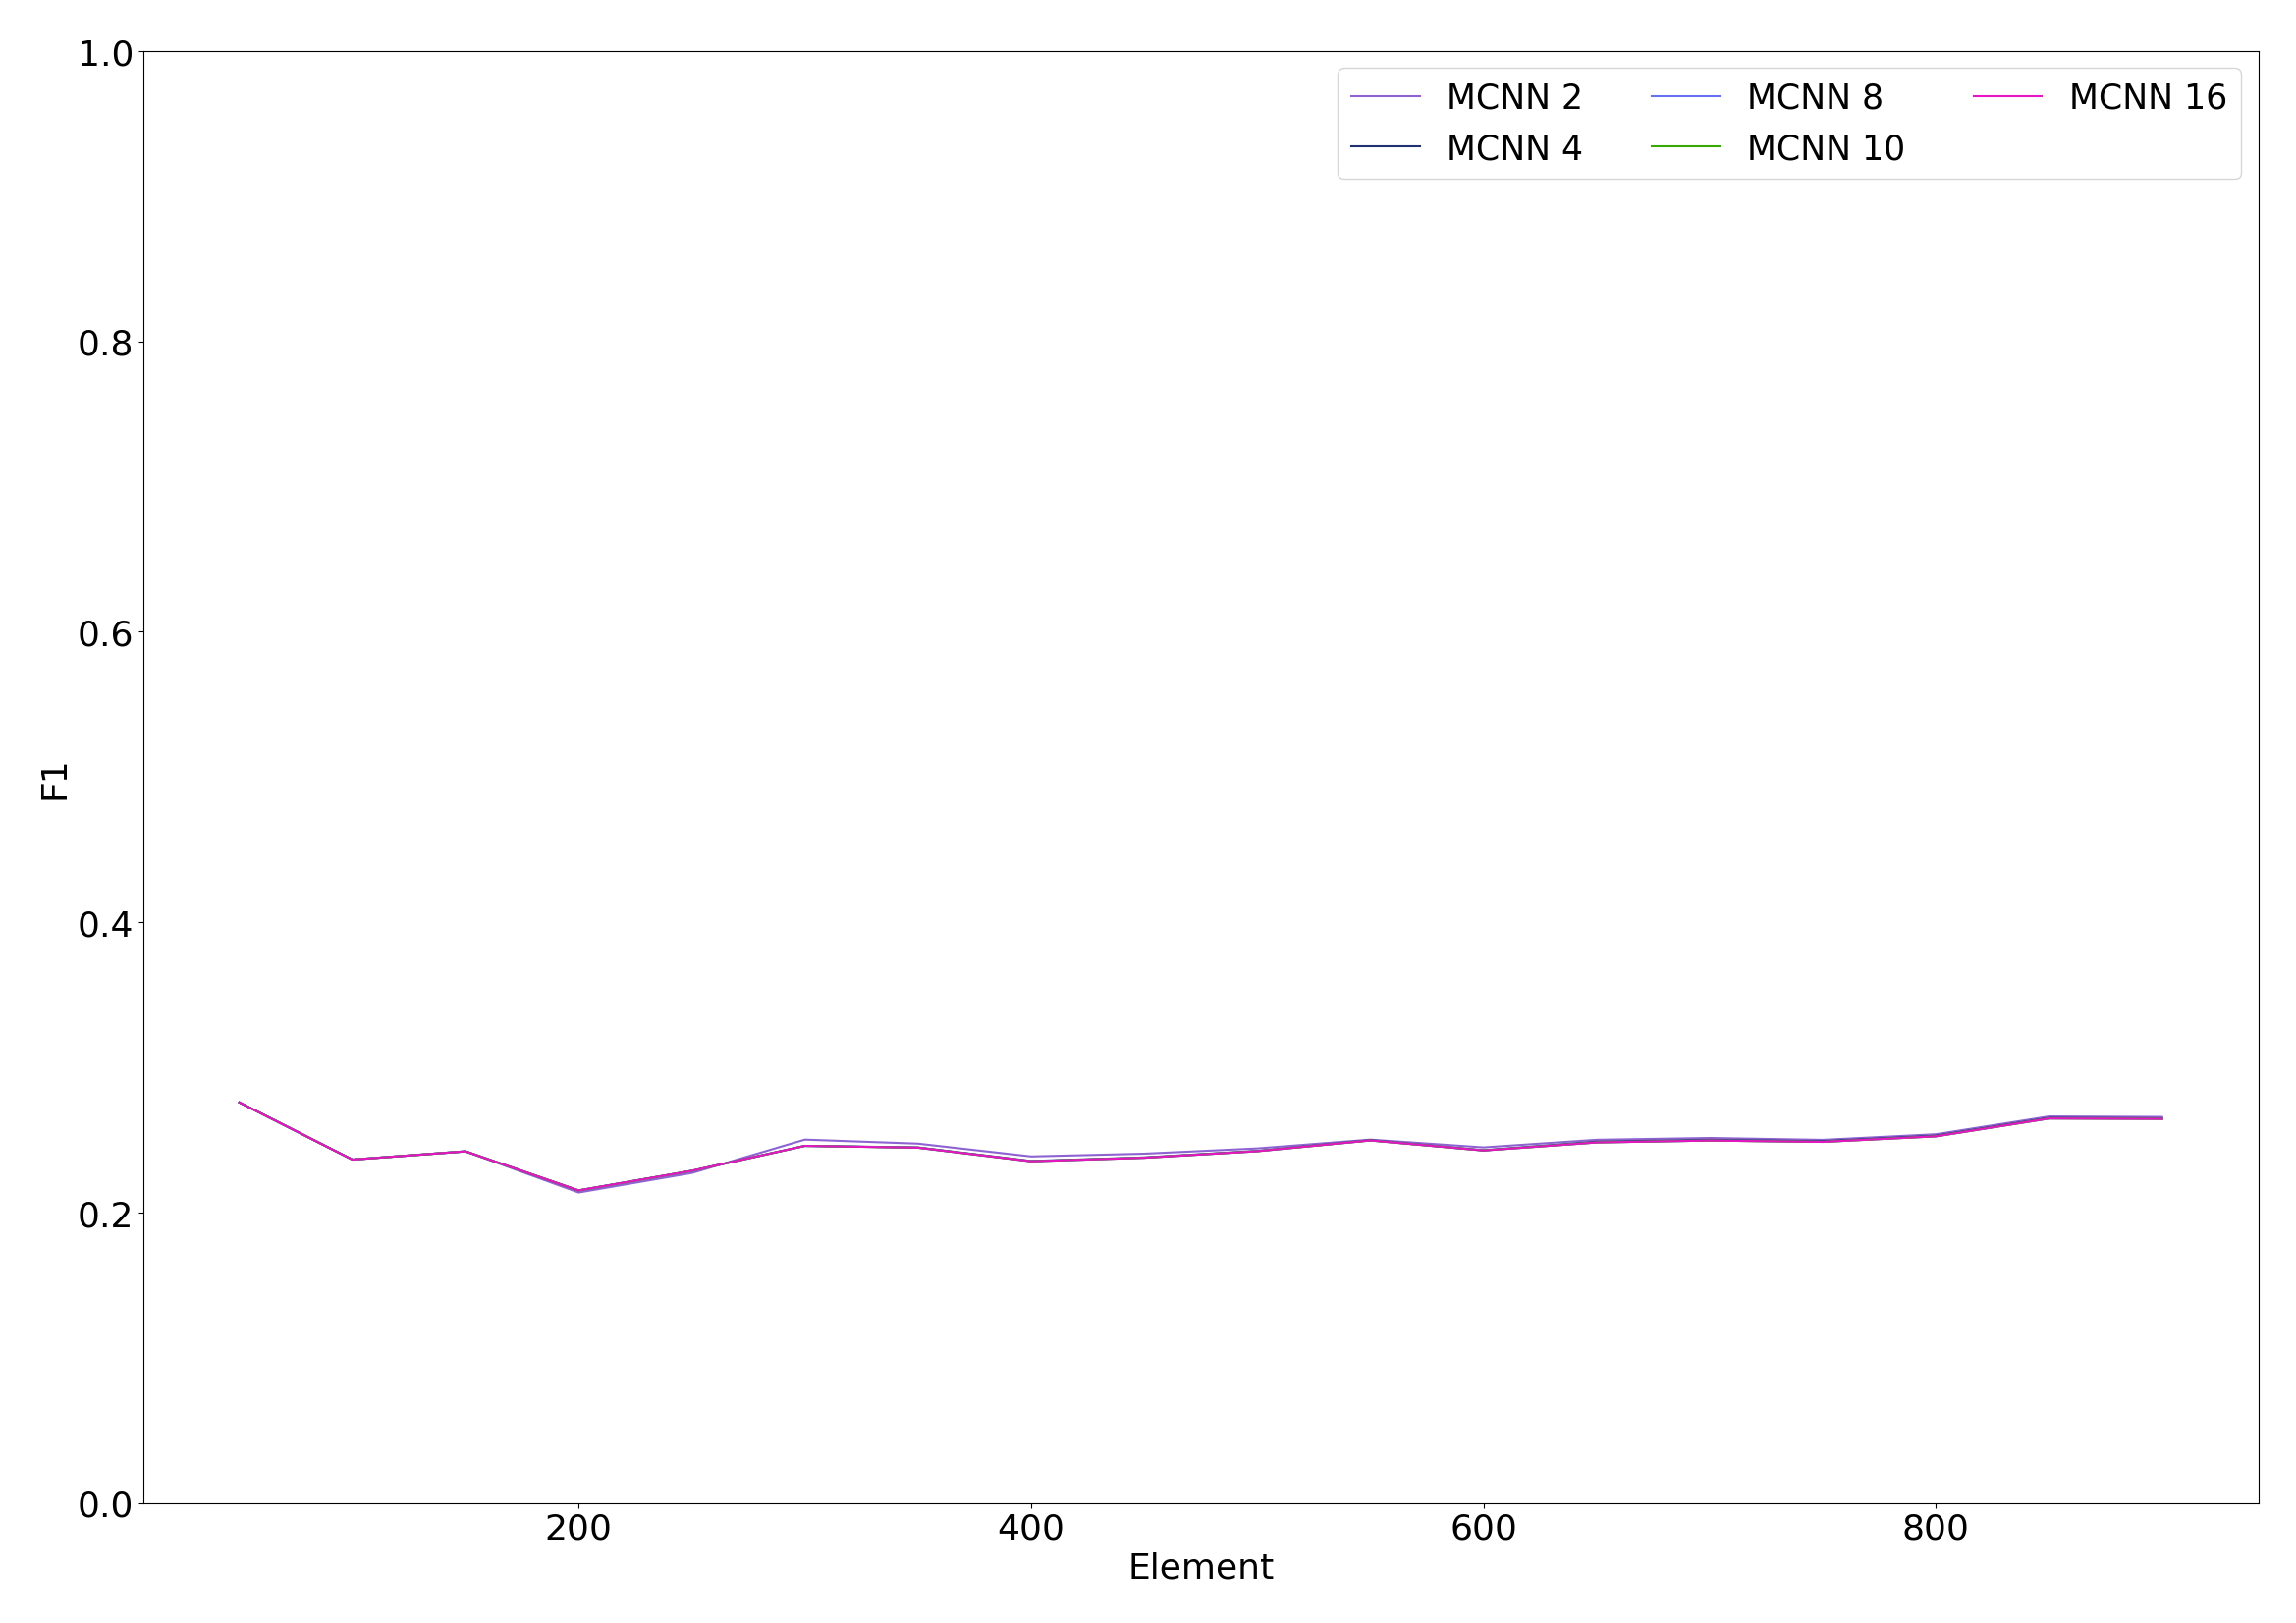
\includegraphics[width=\linewidth]{figures/calibration_mcnn_10.png}
		 \caption{10 clusters}
	 \end{subfigure}
	\caption{Error threshold tuning of \mcnn with first subject of \banosdataset dataset.}
	\label{fig:mcnn-tuning-error}
\end{figure}

Figure~\ref{fig:mondrian-tuning} shows the impact of the \mondrianforest hyperparameters on
the classification performance. 
The base count hyperparameter (Figure~\ref{fig:mondrian-base-count}) has a
very substantial impact on classification performance; the smallest value
(0.0) results in the best performance. On the contrary, the
budget hyperparameter (Figure~\ref{fig:mondrian-budget}) only has a
moderate impact on classification; the best value is 0.2. Finally, the discount hyperparameter
(Figure~\ref{fig:mondrian-discount}) has a negligible impact on the
performance; the best-performing value is 0.1.

\begin{figure}
	 \centering
	 \begin{subfigure}[b]{0.49\textwidth}
		\centering
		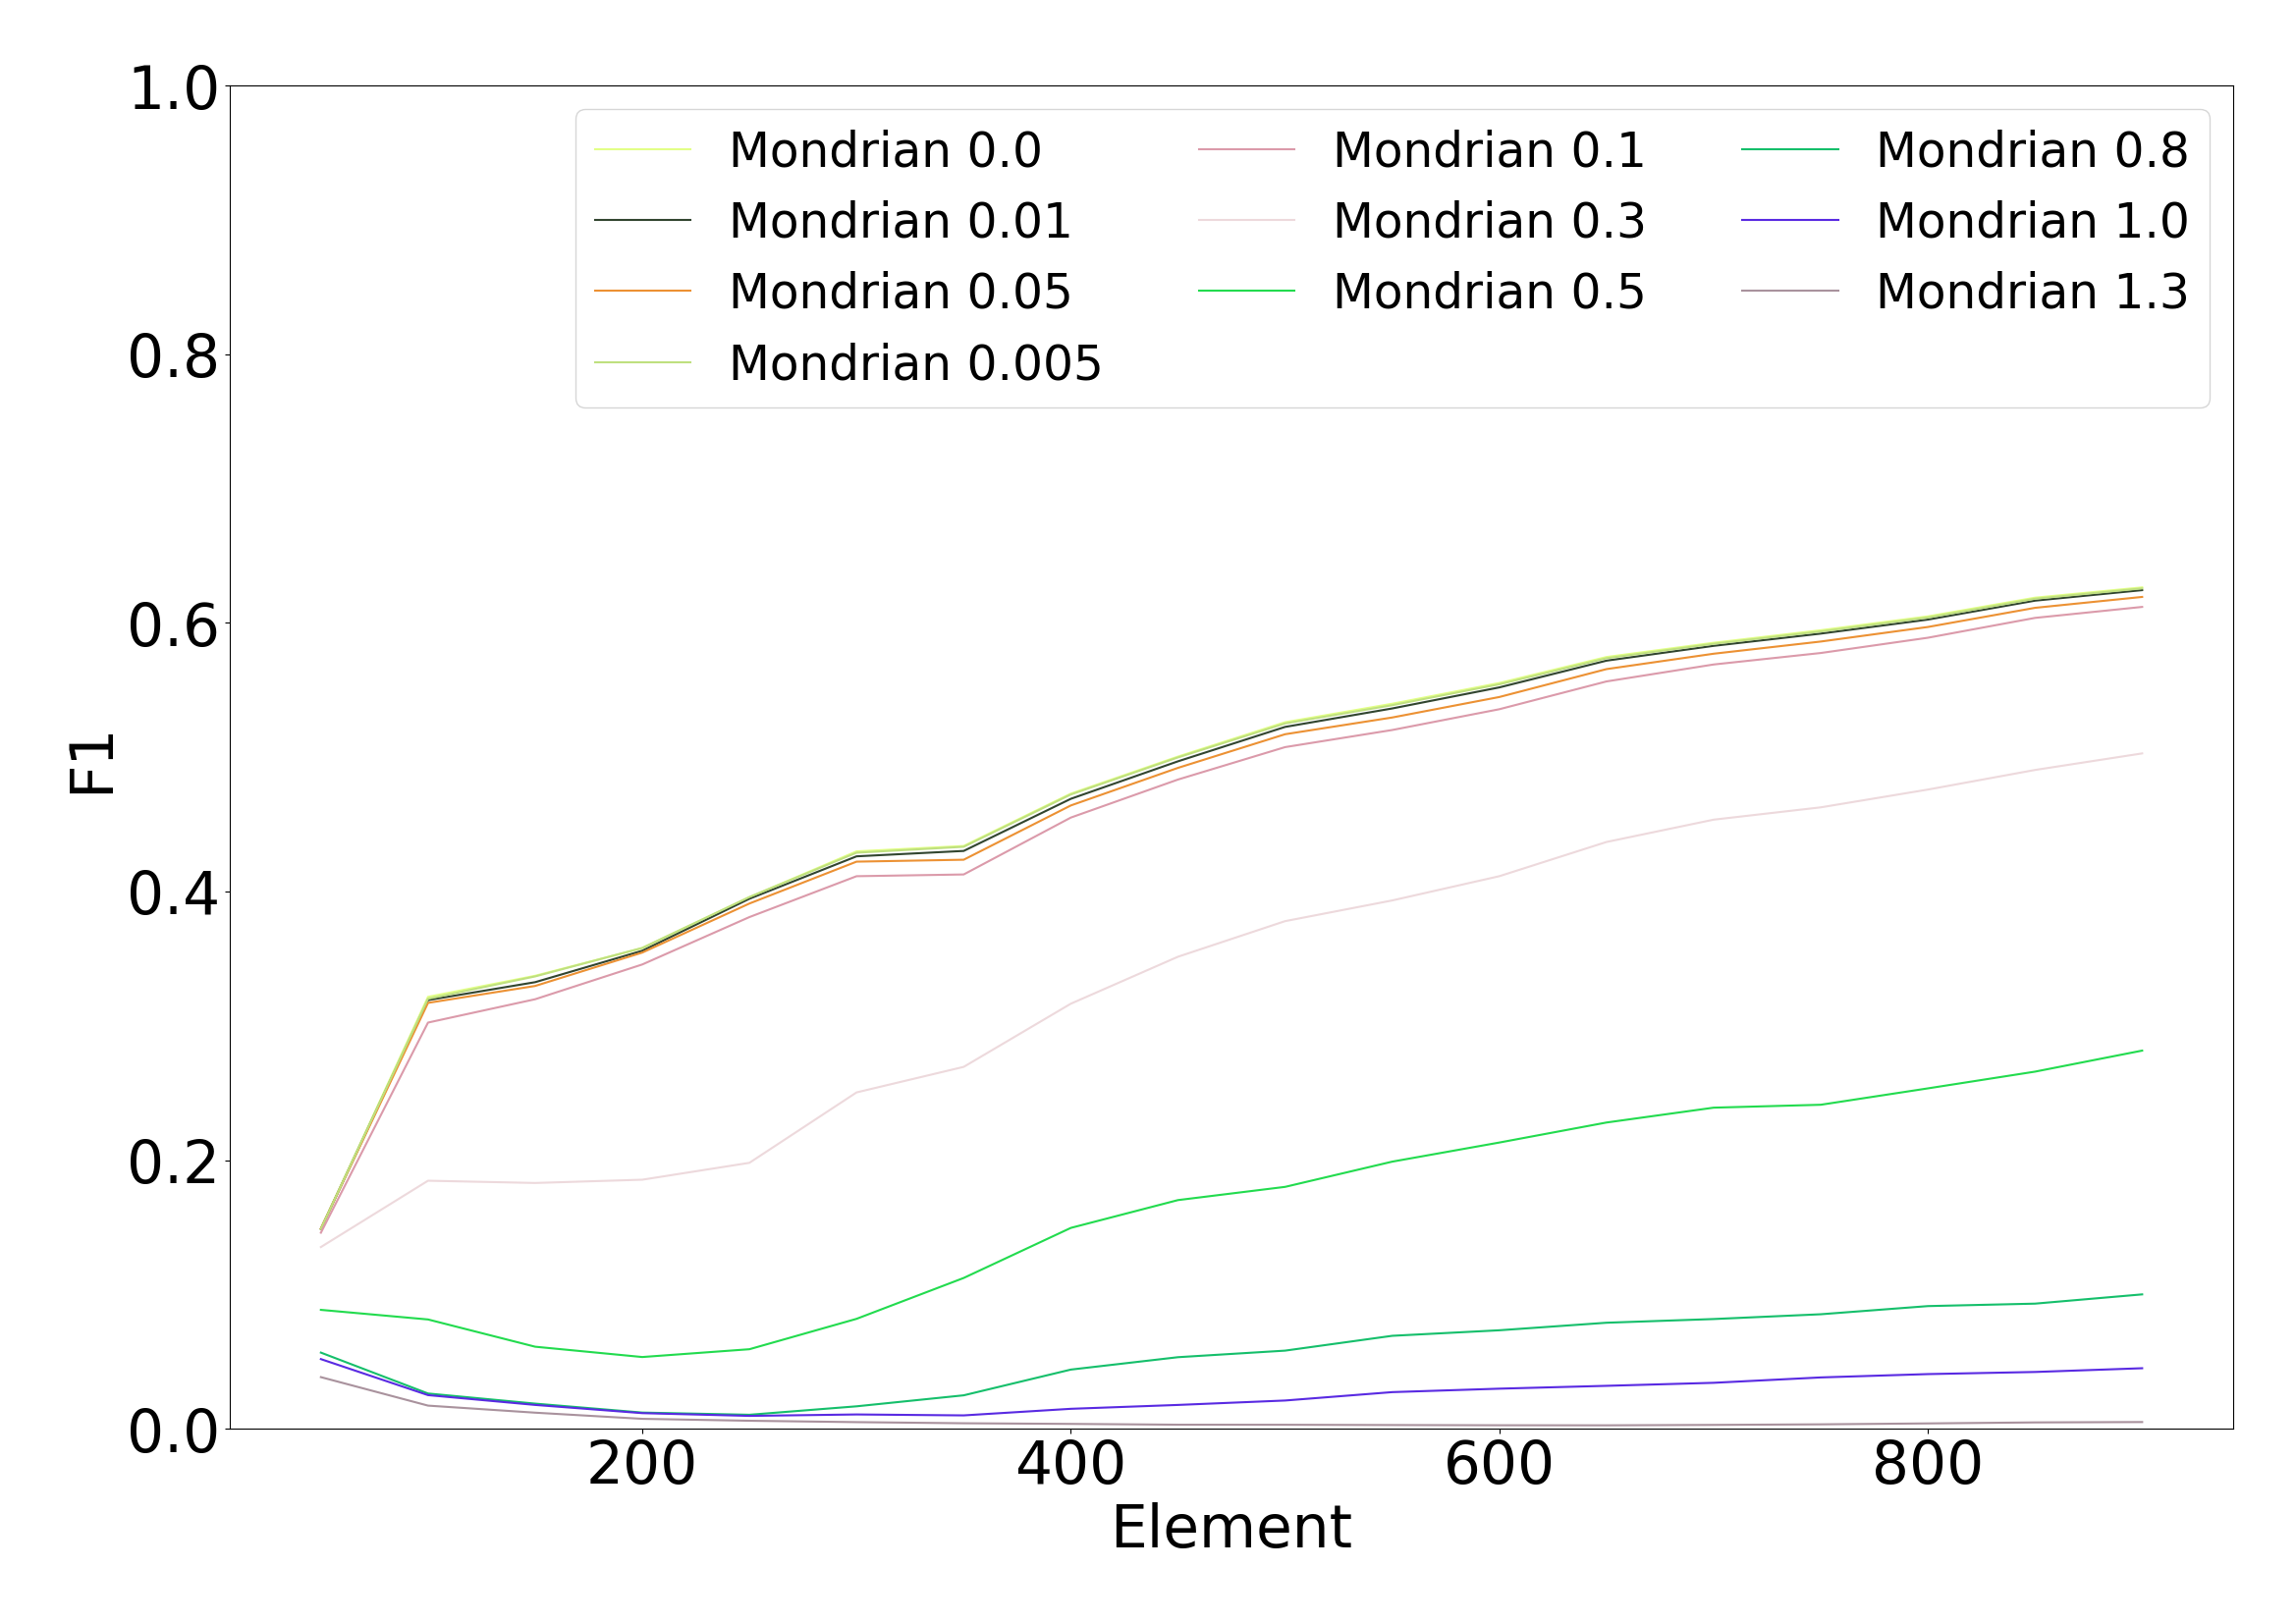
\includegraphics[width=\textwidth]{figures/calibration_mondrian_base.png}
		\caption{Impact of the base count with 10 trees, a budget of $1.0$, and a discount factor of $0.2$.} 
		\label{fig:mondrian-base-count}
	\end{subfigure}
	\hfill
	 \begin{subfigure}[b]{0.49\textwidth}
		 \centering
		 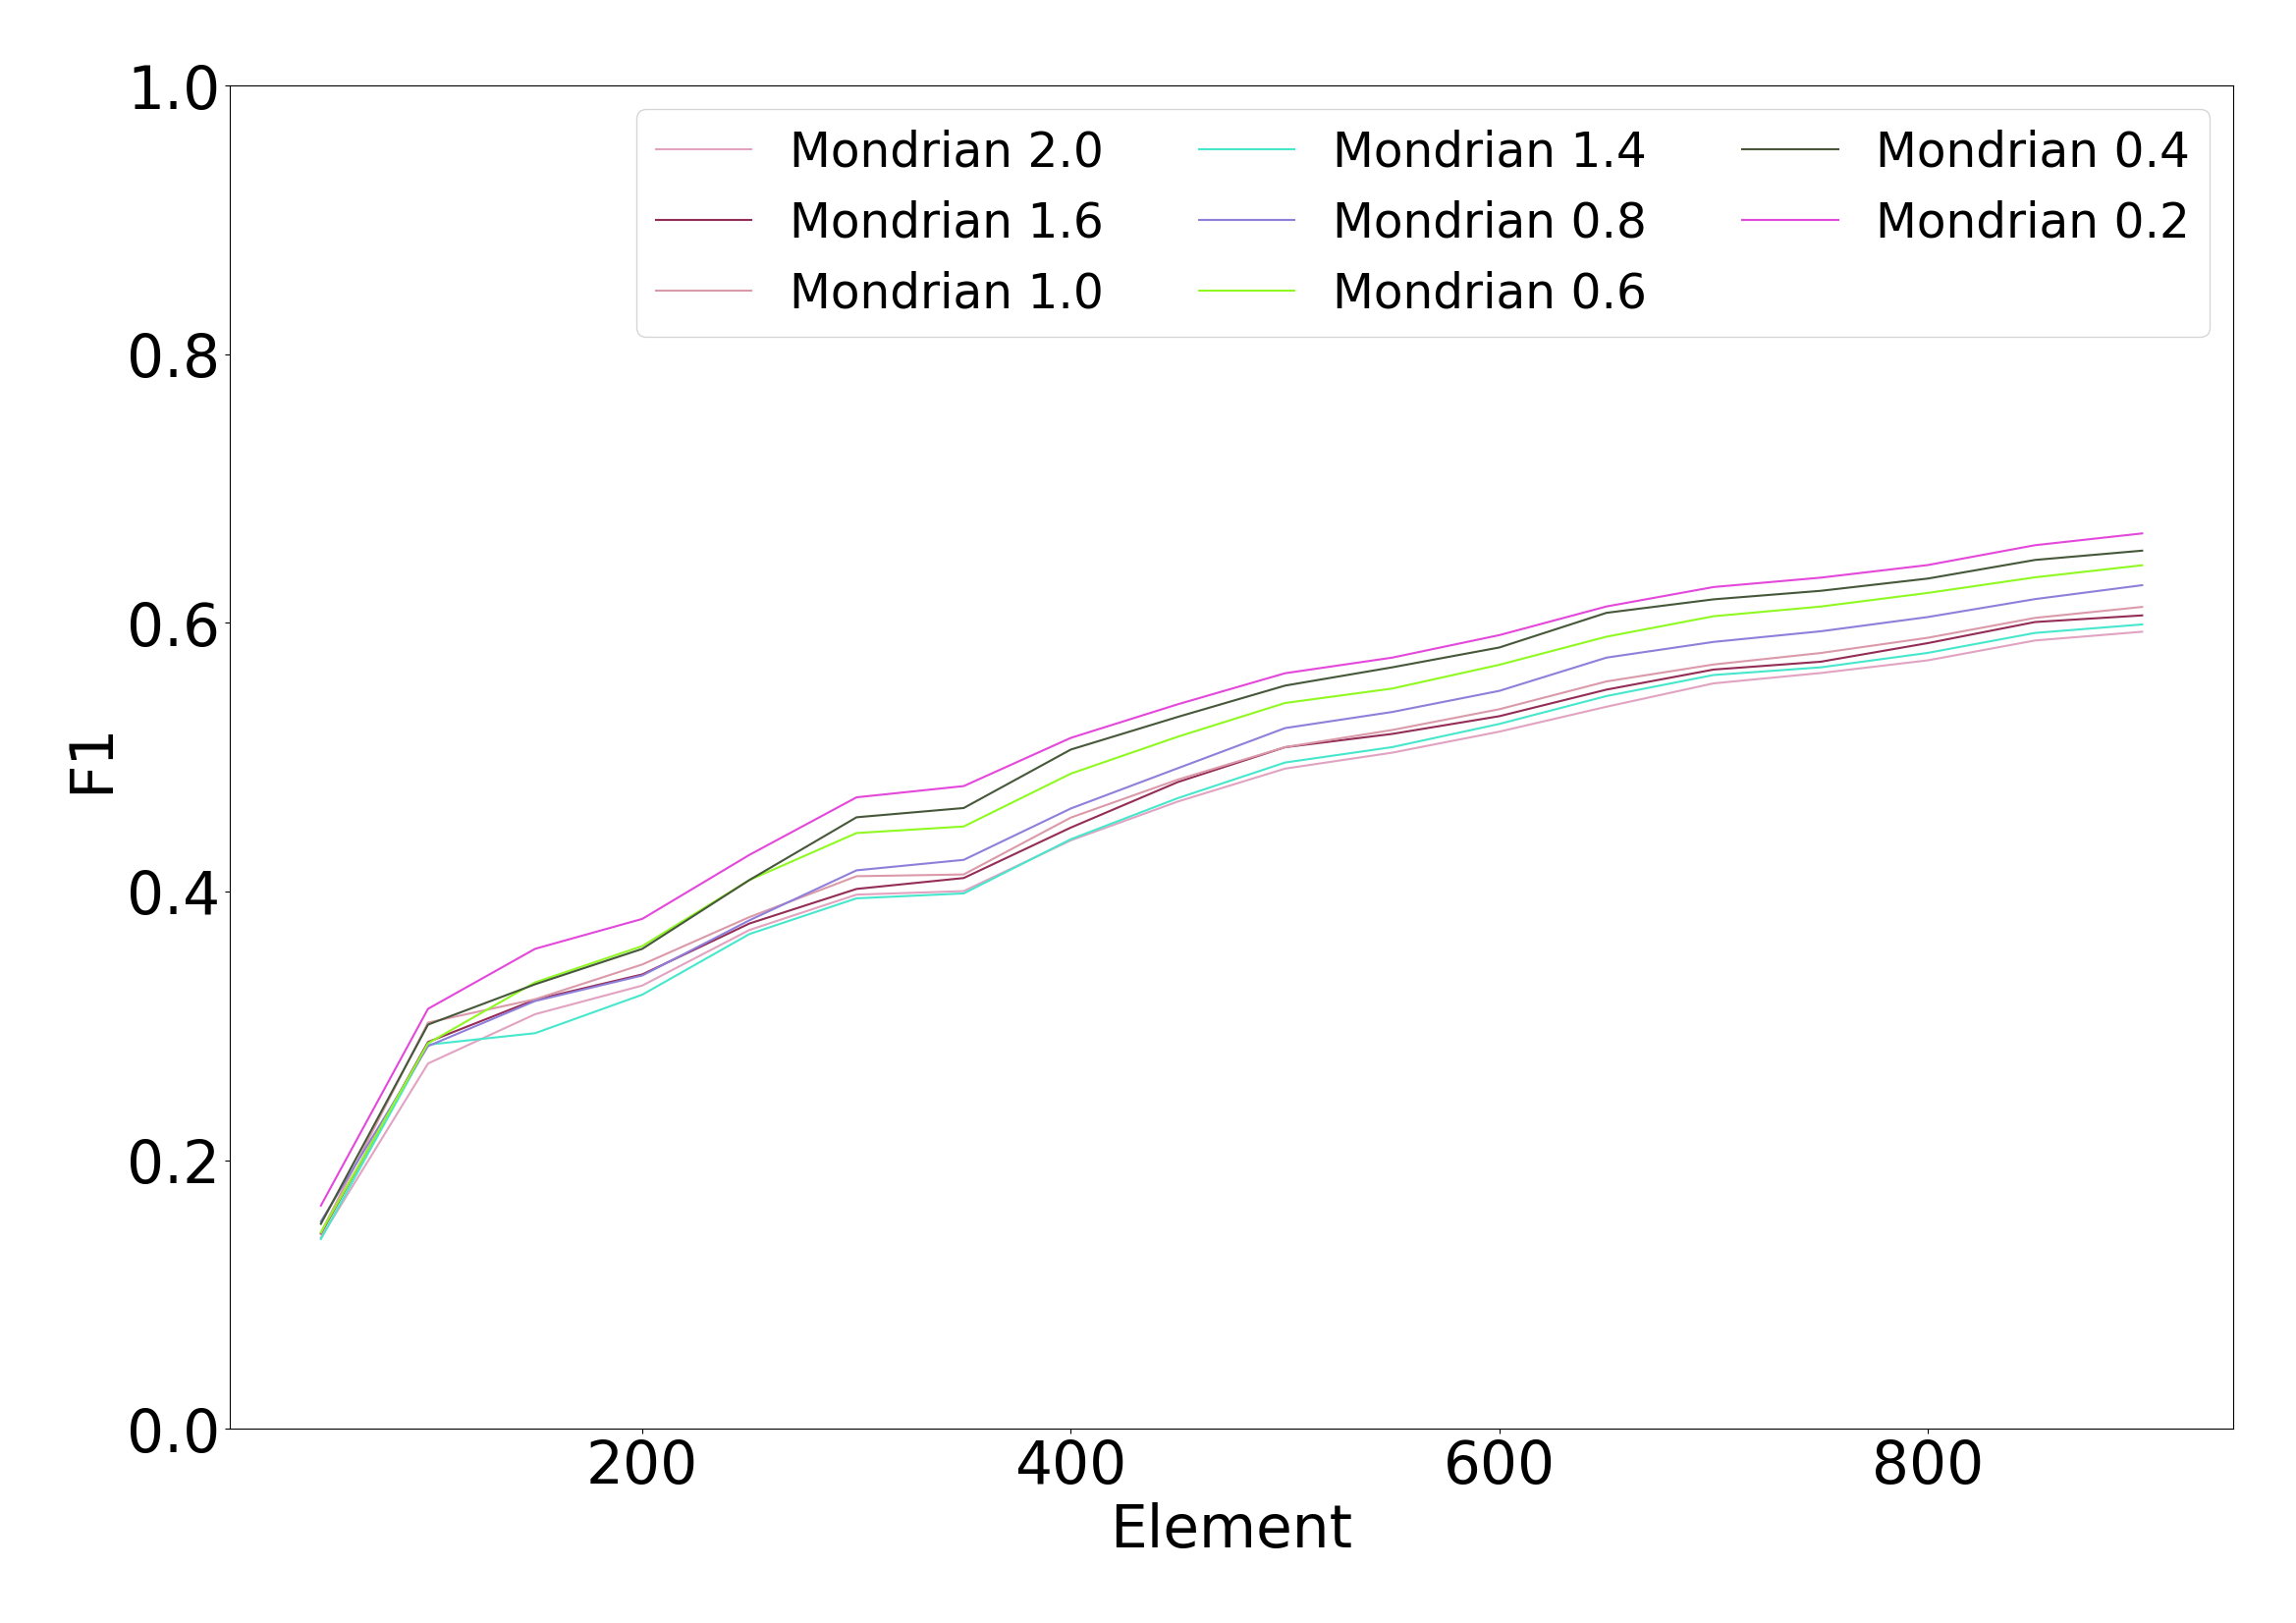
\includegraphics[width=\textwidth]{figures/calibration_mondrian_lifetime.png}
		 \caption{Impact of the budget with 10 trees, a base count of $0.1$, and discount factor of $0.2$.}
		 \label{fig:mondrian-budget}
	 \end{subfigure}
	 \hfill
	 \begin{subfigure}[b]{0.49\textwidth}
		 \centering
		 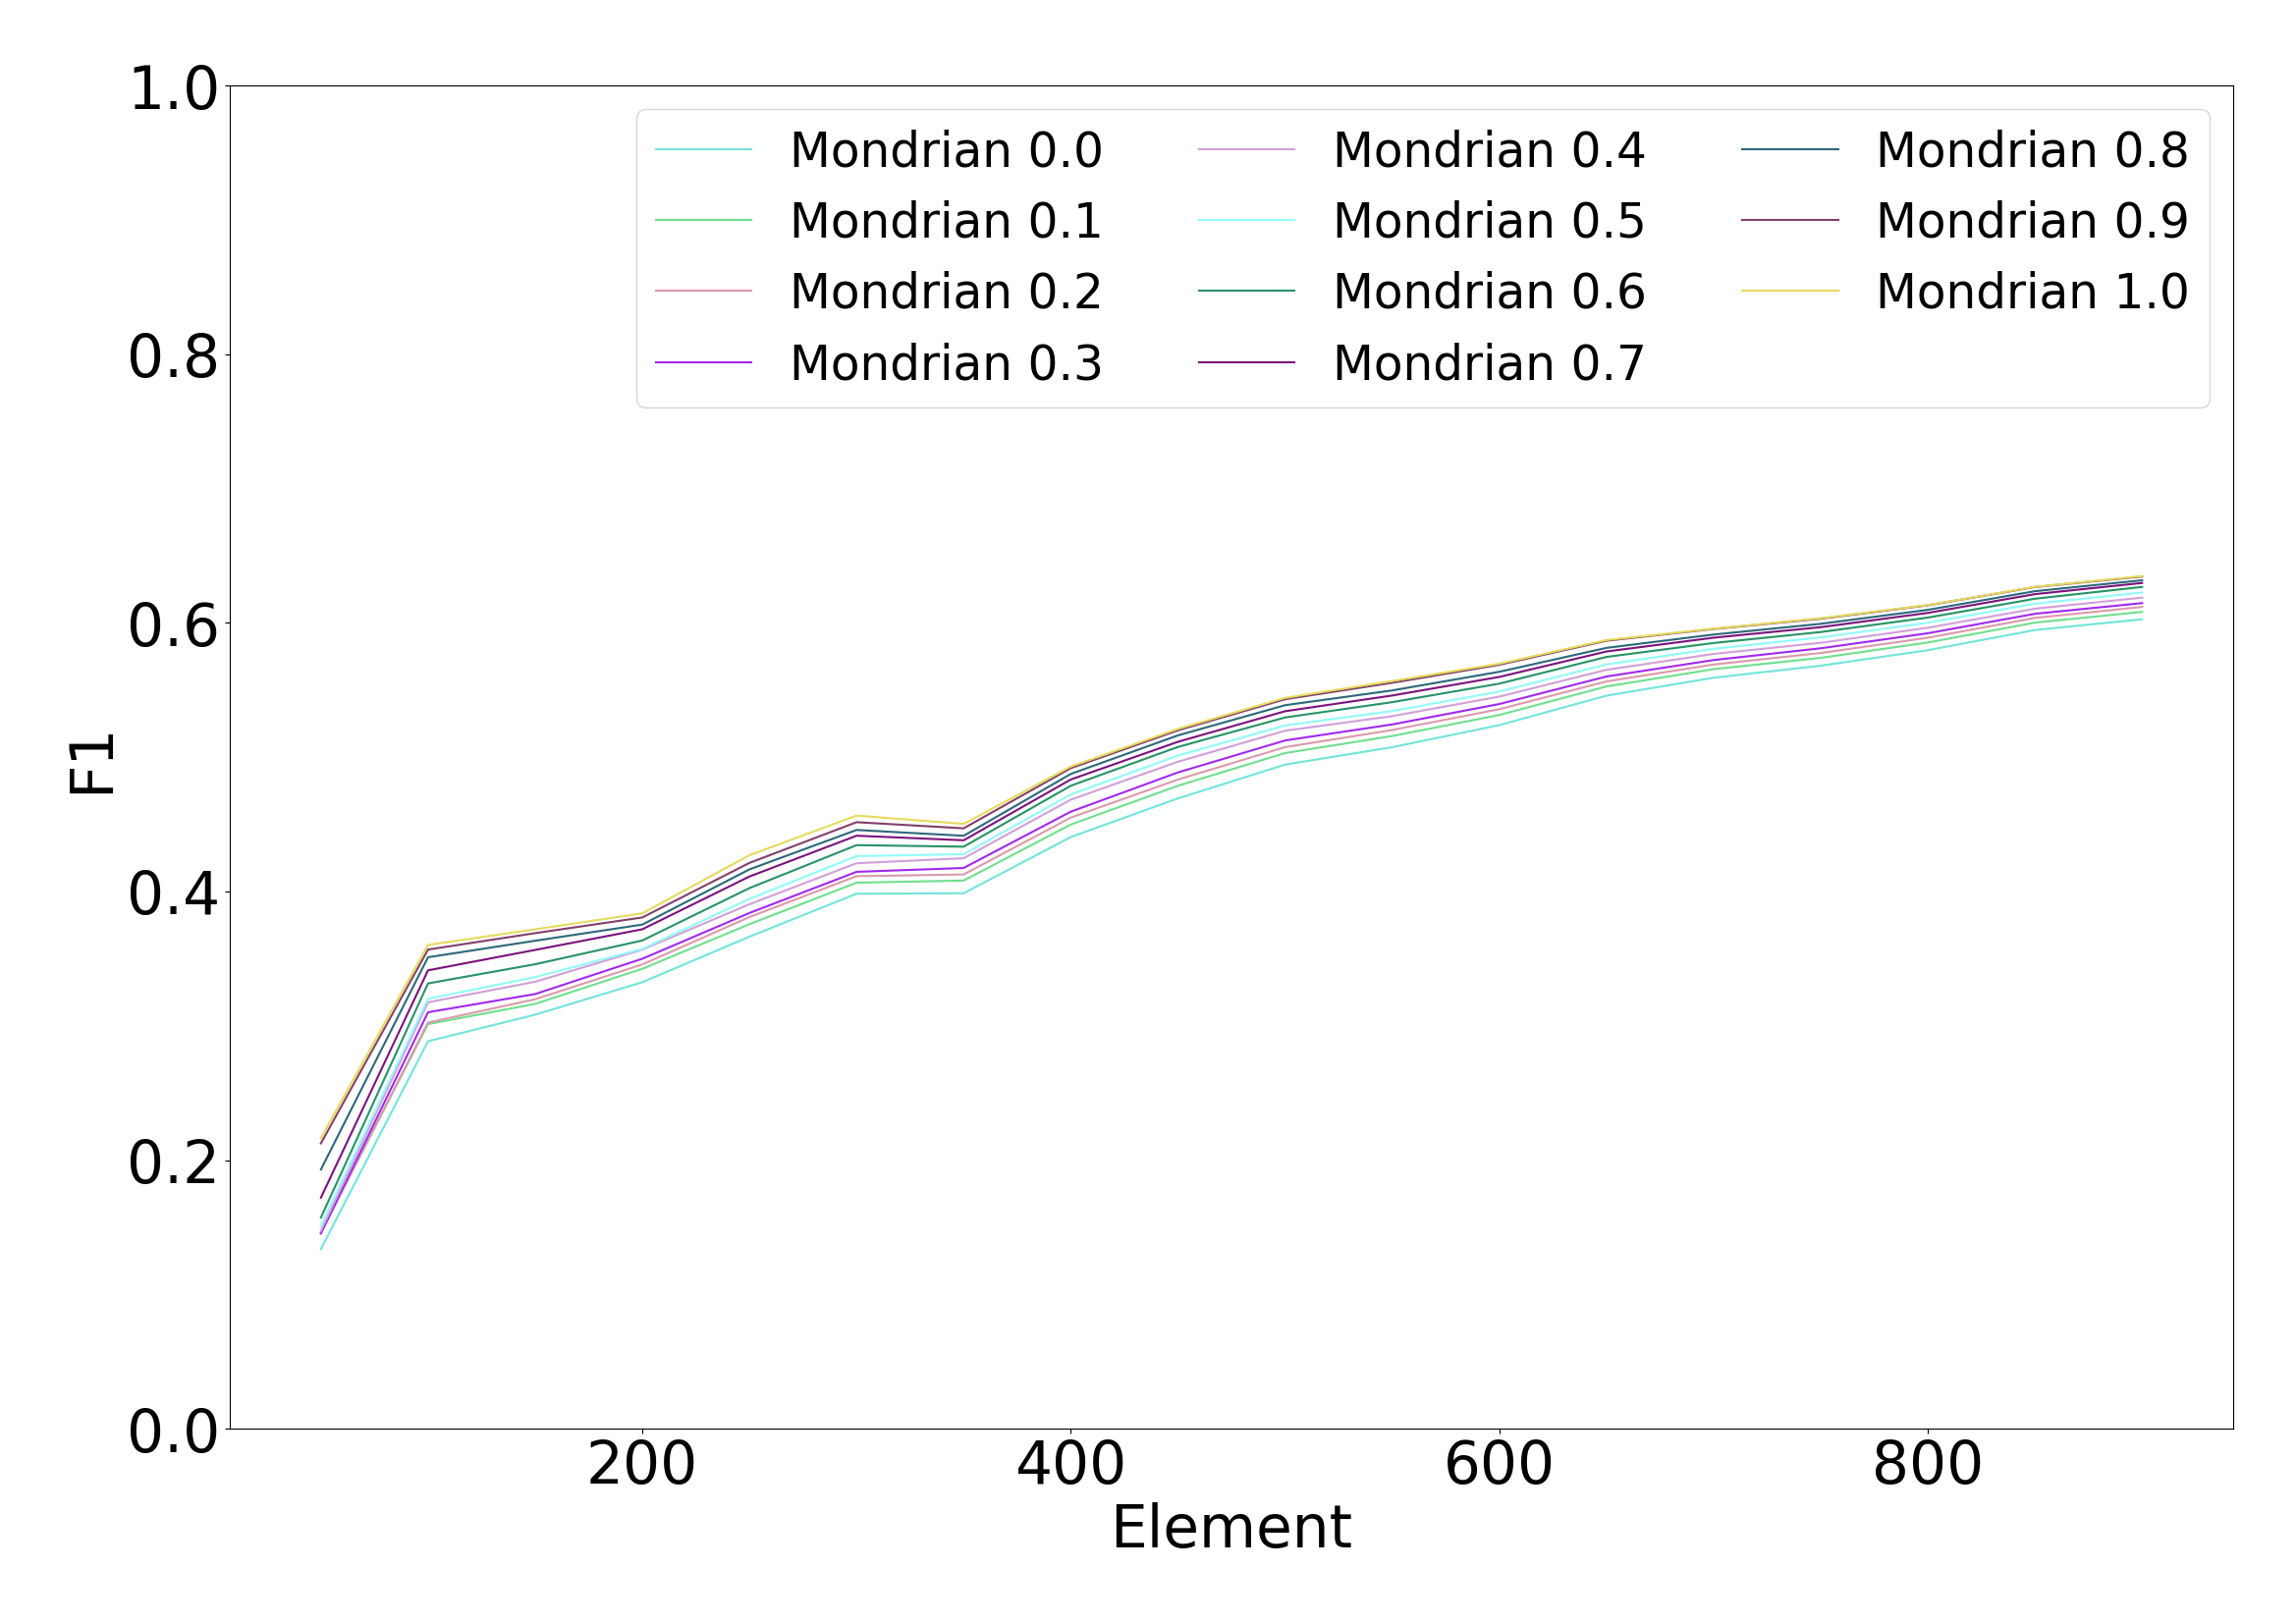
\includegraphics[width=\textwidth]{figures/calibration_mondrian_discount.png}
		 \caption{Impact of the discount factor with 10 trees, a budget of $1.0$, and a base count of $0.1$.}
		 \label{fig:mondrian-discount}
	 \end{subfigure}
		\caption{Hyperparameters tuning for Mondrian with first subject of \banosdataset dataset.}
		\label{fig:mondrian-tuning}
\end{figure}


% vim: tw=80 ts=2

\section{Discussion}
%Mondrian has the greatest F1-scores, however, slow runtime
From this study we observed that the Mondrian algorithm presents the best classification performances.
However, we have also noticed that it is the slowest classifier.

%Link with litterature

%All F1-scores remains low
We notice that most of the f1-scores are low.

%Pk 1 capteur
%Pk 3 axes.

%Puissance, pk pas de différence significative (platform)
Section~\ref{sec:power} shows no power difference between classifier. This
observation is explainable by two factors. The plateform used is too powerful
and it was already working at minimal power. Indeed, to ensure no disturbance
by a background process, we run the classifier on an isolated cluster node with
eight cores. Therefore, the power difference on one core is not noticable.

Another reason is regarding the dataset size. Indeed, the slowest run is about
10 seconds with 50 Mondrian trees on \recofitdataset dataset.  Such short
execution does not leave the time for the CPU to switch P-states because it
barely warms a core.

% Mémoire contrainte, partir sur l'exploration : toute xp faite à mémoire constante, qu'est-ce qu'il se passe ac' + de mémoire.
In section~\ref{sec:result-memory}, we differenciate bounded memory and
constant space complexity because in the first case, a limited amount of memory
may impact the classifier performances. On the other hand, a constant space
complexity is a feature of a classifier and its performances are not expected
to change no  matter the amount of memory available. The classifier is simply
supposed to fail without the required amount of memory.


%Conclusion : Improve mondrian runtime






\section{Conclusion}

We conclude that the \hoeffdingtree, the \mondrianforest, and the
\naivebayes data stream classifiers have an overall superiority over the
\FNN and the \mcnns ones for Human Activity Recognition.  However, the
predictions performances remain quite low compared to their offline
counterpart, and they vary substantially between datasets. Noticeably, the
\hoeffdingtree and the \mcnns classifiers are more resilient to concept drift that the
other ones.

Regarding memory consumption, only the \mcnns and \naivebayes classifiers
were found to have a negligible memory footprint, in the order of a few
kilobytes, which is compatible with connected objects. Conversely, the
memory consumed by a \mondrianforest, a \FNN or a \hoeffdingtree is in the
order of 100~kB, which would only be available on some connected objects.
In addition, the classification performance of a \mondrianforest is
strongly modulated by the amount of memory allocated. With enough memory, a
\mondrianforest is likely to match or exceed the performance of the
\hoeffdingtree and \naivebayes classifiers.

The amount of energy consumed by classifiers is mostly impacted by their
runtime, as all power consumptions were found comparable. The
\hoeffdingtree and \mondrianforest are substantially slower than the other
classifiers, with runtimes in the order of 0.35~ms/element. 

Future research will focus on reducing the memory requirements and runtime
of the \hoeffdingtree and the \mondrianforest classifiers. In addition to
improving the deployability of these classifiers on connected objects, this
would also potentially improve their classification performance, since
memory remains a bottleneck in the \mondrianforest.

\section*{Acknowledgement}
This work was funded by a Strategic Project Grant of
the Natural Sciences and Engineering Research Council of
Canada


\bibliographystyle{plain}
\bibliography{paper}
\end{document}

% vim: tw=50 ts=2

